\documentclass[english,headsepline,footsepline,12pt]{scrreprt}

% --- Core packages -------------------------------------------------
\usepackage[utf8]{inputenc}
\usepackage[T1]{fontenc}
\usepackage{times}
\usepackage[english]{babel}
\usepackage{csquotes}

% --- Layout & graphics --------------------------------------------
\usepackage{graphicx,color}
\usepackage{xcolor}
\usepackage{url}
% Breakable monospace for code identifiers. Lines may break at an underscore
% and no hyphen is inserted, so an identifier is never misread. Use
% \code{some_identifier} in prose and tables; \texttt stays for short words.
\DeclareUrlCommand\code{\urlstyle{tt}}
\usepackage{verbatim}
\usepackage{longtable}
\usepackage{tabularx}
\usepackage{booktabs}
\usepackage{multicol}
\usepackage[automark]{scrlayer-scrpage}

% --- Math ----------------------------------------------------------
\usepackage{latexsym}
\usepackage{amsmath}
\usepackage{amssymb}

% --- Algorithms, code, diagrams -----------------------------------
\usepackage{algorithm}
\usepackage{algorithmic}
\usepackage{listings}
\usepackage{tikz}
\usetikzlibrary{arrows.meta,positioning,shapes.geometric,fit,calc}

% --- Cross-references (load LAST) ---------------------------------
\usepackage[breaklinks,colorlinks=true,citecolor=blue,linkcolor=blue,urlcolor=blue,filecolor=blue]{hyperref}

% --- Bibliography (biblatex, bibtex backend so Tectonic runs it) ---
\usepackage[backend=bibtex,style=numeric-comp,sorting=nyt,maxbibnames=99,giveninits=true]{biblatex}
\addbibresource{bibs/litDB.bib}

\usepackage{cleveref}

% --- listings defaults --------------------------------------------
\lstset{
  basicstyle=\ttfamily\footnotesize,
  breaklines=true,
  frame=single,
  showstringspaces=false,
  tabsize=2,
  captionpos=b,
}

% --- Header / footer ----------------------------------------------
\clearpairofpagestyles
\chead{\headmark}
\ofoot[\pagemark]{\pagemark}
\ifoot{\invnr}
\pagestyle{scrheadings}

% --- Page geometry -------------------------------------------------
\setlength{\topmargin}{1.5cm}
\setlength{\headheight}{12pt}
\setlength{\headsep}{20pt}
\setlength{\topskip}{12pt}
\setlength{\evensidemargin}{0pt}
\setlength{\oddsidemargin}{0pt}
\setlength{\textheight}{240mm}
\setlength{\textwidth}{160mm}
\setlength{\voffset}{-2cm}
\setlength{\parindent}{0pt}
\setlength{\parskip}{6pt}

% Author / thesis metadata. Fill in TODOs before final build.

\newcommand{\saauthor}{Anik Dewanje}
\newcommand{\matrikel}{64746}
\newcommand{\sathema}{Design and Evaluation of a Database-Centric Agentic Architecture for Nursing Home Evacuation Coordination in Storm Surge Scenarios}

\newcommand{\saprof}{Prof. Dr.-Ing. habil. Kai-Uwe Sattler}
\newcommand{\sabetreuer}{M. Sc. Saba Zamankhani}

\newcommand{\invnr}{TODO-INVENTORY-NUMBER}


%%%%%%%%%%%%%%%%%%%%%%%%%%%%%%%%%%%%%%%%%%%%%%%%%%%%%%%%%%%%%%%%%

\begin{document}

% --- Front matter --------------------------------------------------
\begin{titlepage}

\begin{center}

\includegraphics[height=2cm]{pics/logo-thi.jpg}
\vspace{1cm}

TECHNISCHE UNIVERSITÄT ILMENAU\\
Institute of Applied Computer Science \\
Department of Computer Science and Automation\\
Databases and Information Systems Group

\vspace{4cm}

{\large Master's thesis} \\ 
\vspace{1cm}
{\LARGE \normalfont \bfseries \sathema} \\
\vspace{1cm}
{presented by} \\
\vspace{0.5cm}
{\large \saauthor}\\
{\large Matriculation No \matrikel}
\vspace{2cm}

Supervisor: \\
\vspace{0.5cm}
\saprof \\
\sabetreuer \\

\vspace{1cm}

Ilmenau, den \today
\end{center}

\end{titlepage}

\pagenumbering{roman}

\chapter*{Abstract}
\addcontentsline{toc}{chapter}{Abstract}

% TODO: 1 page. State problem, approach, contributions, key results.

\chapter*{Acknowledgements}
\addcontentsline{toc}{chapter}{Acknowledgements}

% TODO: Optional.


\tableofcontents
\listoffigures
\listoftables
\newpage

% --- Main matter ---------------------------------------------------
\pagenumbering{arabic}

% Chapter order follows thesis-pack/README.md. Two chapters were added on
% 2026-09-22: validity (from 08-validity/PARITY.md) and the methods critique
% (from 09-method/EVALUATION_PROTOCOL_V2.md). The instrument implementation
% (10-instrument) folds into the evaluation chapter, which already covers the
% scorer and the harness.

\chapter{Introduction}
\label{ch:intro}

% ===========================================================================
% FRAMING, SETTLED WITH THE SUPERVISOR 2026-09-22.
%
% This is a DESIGN-AND-EVALUATION study, not a hypothesis-confirmation study.
% The motivation was to design an agentic simulation architecture, evaluate it
% honestly against an old-style scripted baseline, and report what was learned
% either way. A negative answer is a result here, not a failure.
%
% Write the whole thesis in that voice. Never apologise for the outcome.
% ===========================================================================

\section{Motivation}
\label{sec:intro:motivation}
% Why evacuation coordination is hard: heterogeneous organisations, local
% information, a hard deadline, and a disruption space too large to enumerate.
% Why the old style falls short: a pre-scripted workflow can only cover the
% cases its author thought of.
% Why an agentic architecture is the obvious thing to try: agents that reason
% over a shared database can in principle answer a disruption nobody scripted.
% END ON THE OPEN QUESTION, not on a promise: nobody had measured whether that
% promise survives contact with a scored evacuation.

\section{Problem Statement}
\label{sec:intro:problem}
% The concrete problem: move 100 residents of a riverside nursing home to
% shelters before a forecast storm surge, using resources owned by eight
% different organisations, when the plan must change mid-operation.

\section{Research Questions}
\label{sec:intro:rq}
% ---------------------------------------------------------------------------
% THE FOUR QUESTIONS, AS SETTLED. Each has an answer in this thesis. Write the
% question here and the answer in the chapter named, then again in the
% conclusion. Do not hedge any of the four.
%
% RQ1  Can a database-centric agentic architecture coordinate an evacuation
%      BETTER than an old-style scripted workflow baseline?
%      ANSWER: No, on the pre-registered primary outcome.
%      -> Chapter~\ref{ch:results}. Gate 1 fails 26 of 27 cells. The baseline
%         saved every resident in every novel run; the best agentic
%         configuration saved 90 %.
%      -> And it is worse than that: against a null policy that ignores every
%         disruption, agentic regret is negative in all 15 novel cells and 68
%         of 150 runs came out WORSE THAN DOING NOTHING.
%      -> BOUNDARY, state it in the same breath (Chapter~\ref{ch:critique}):
%         no scenario in this thesis ever REQUIRED adaptation, so this answers
%         "did it win here", not "can it ever win".
%
% RQ2  If not, why not? Where does the deficit come from?
%      ANSWER: A COMMITMENT failure, not a comprehension failure.
%      -> Chapter~\ref{ch:results} and Chapter~\ref{ch:critique}.
%      -> The agents understood the disruption. They were told the right
%         population in 150 of 150 runs, closed 93.8 % of addressed requests,
%         dispatched the same number of missions in failing and succeeding
%         runs, and used the reserve bus in 100 % of runs.
%      -> What they could not do is carry ONE COMMITTED PLAN to delivery.
%         Losses are quantised at whole bus-loads: of 150 runs, 102 delivered
%         everyone, 19 delivered exactly 50, 18 delivered exactly 90.
%      -> Plan revisions band monotonically against delivery: 90 % full
%         delivery at the minimum revision count, 32 % at six or more.
%         r(plan revisions, S) = -0.408, the strongest non-definitional
%         predictor in the data.
%      -> THE IRONY TO NAME OUT LOUD: re-planning on disruption is the
%         architecture's advertised capability, and on these scenarios the
%         correct number of re-plans was ZERO.
%
% RQ3  What would have to change to make an agentic emergency simulation
%      better?
%      ANSWER: constrain commitment, and test on scenarios that discriminate.
%      -> Chapter~\ref{ch:conclusion}, future work.
%      -> The named experiment: a COMMITMENT-CONSTRAINED VARIANT. Cap re-plans,
%         or forbid cancelling a leg already in flight, run against the same
%         scenarios under the same models. One campaign, no new scenario
%         authoring. It is also what would settle the causal direction, which
%         this thesis explicitly does NOT establish.
%      -> Plus: Gate 0 as a precondition on scenario authoring, a larger k, and
%         more than one SIM_TIME_SCALE.
%
% RQ4  What should be considered when designing an AI agentic emergency
%      simulation?
%      ANSWER: Chapter~\ref{ch:design}. This is the generalisable deliverable
%      and the part that stops being about one nursing home in Hamburg.
%
% ---------------------------------------------------------------------------
% The four engineering sub-questions from the original proposal still hold and
% are answered by the architecture chapters. Keep them, subordinate to RQ1-RQ4:
%   1. Data modelling of actors, states, events, dependencies
%      -> Chapter~\ref{ch:data}
%   2. Integration of heterogeneous organisational agents
%      -> Chapter~\ref{ch:agentic}
%   3. Persistent structures for runtime control AND evaluation
%      -> Sections~\ref{sec:data:eventlog} and \ref{sec:data:evalbackbone}
%   4. Comparative performance, agentic vs workflow
%      -> Chapters~\ref{ch:eval} and \ref{ch:results}

\section{Contributions}
\label{sec:intro:contributions}
% FOUR contributions. State them as claims the thesis actually supports.
%
%  1. ARTEFACT. A database-centric agentic architecture for multi-organisation
%     evacuation coordination: 10 agents across 8 organisations, Postgres as the
%     single source of truth and the active message broker, built and running.
%     Plus a doctrine-grounded workflow baseline that reaches audited parity
%     with it on the shared surface (Chapter~\ref{ch:validity}).
%
%  2. EMPIRICAL. The first scored head-to-head of the two on a common
%     evacuation case: 310 runs, 7 scenarios, pre-registered, deterministically
%     scored. The agentic architecture does NOT outperform the scripted
%     baseline, and underperforms a null policy.
%     (This replaces the proposal's expected finding. Say so plainly.)
%
%  3. DIAGNOSTIC. A measured account of WHY, which is the part a future builder
%     can use: the deficit is commitment, not comprehension, and plan churn is
%     its strongest correlate.
%
%  4. METHODOLOGICAL. The shared append-only event log that makes the
%     comparison fair, auditable and replayable; and Gate 0, a treatment-
%     validity check that catches a disruption which does not discriminate
%     a replanner from a non-replanner BEFORE it is scored.
%
% NOTE. The proposal expected contribution 2 to read "agentic degrades more
% gracefully". It does not. Do not leave the old wording anywhere.

\section{Scope and Delimitations}
\label{sec:intro:scope}
% Out of scope: resident-level agents (residents are a passive count), heavy
% workflow engines (Camunda/Temporal/Airflow), modelling the flood itself,
% real-time citizen apps.
% Bounded by design: one case study, one facility, one city.
% Bounded by what was run: one SIM_TIME_SCALE (8.4), k = 10, three models with
% a complete novel arm. H4 was not tested. See Chapter~\ref{ch:critique}.

\section{Thesis Outline}
\label{sec:intro:outline}
% One paragraph over Chapters~\ref{ch:background} to \ref{ch:conclusion}.
% Point out the two chapters a reader might not expect and why they are there:
% Chapter~\ref{ch:validity} (the comparison has to be admissible before it is
% interesting) and Chapter~\ref{ch:critique} (the evaluation is itself a
% finding).

\chapter{Background and Related Work}
\label{ch:background}

\section{Evacuation Coordination and Command Doctrine}
\label{sec:bg:evacuation}
% Domain background: disaster response, evacuation planning, vulnerable groups.
% Established command models the workflow baseline is grounded in:
% DV 100 / FwDV 100 (German civil protection) and ICS / NIMS.
% Cite: bigley2001a (ICS as high-reliability organizing), FwDV 100, Plattner,
% Buck/Trainor/Aguirre (critical evaluation of ICS), Moynihan (network governance).
% This section is what makes the baseline "doctrine-grounded" rather than invented.

\section{Multi-Agent Systems}
\label{sec:bg:mas}
% Classical MAS, BDI (Rao & Georgeff), organizational agents, computational
% organization theory (Carley). Positions the "human-organizational agent" choice.

\section{Workflow Flexibility and Unanticipated Exceptions}
\label{sec:bg:workflow}
% BACKBONE SECTION for the baseline's known limits.
% Reichert & Weber (2012): PAIS flexibility, the anticipated-vs-unanticipated
% exception distinction, adaptive workflow (ADEPT/AristaFlow).
% van der Aalst et al. (2009): imperative vs. declarative processes.
% Adams et al. (2007); Marrella SmartPM; Casati; Klein & Dellarocas.
% Also: why heavy engines (Camunda/Temporal/Airflow) are out of scope and a
% plain Python script is the right control condition.

\section{LLM-Driven Agents}
\label{sec:bg:agentic}
% Reasoning-and-acting loops and multi-agent frameworks.
% Cite: yao2023 (ReAct), shinn2023 (Reflexion), park2023 (Generative Agents),
% wu2023 (AutoGen), hong2024 (MetaGPT), li2023 (CAMEL), qian2024 (ChatDev),
% tran2025 + zhuLLMBasedMultiAgentOrchestration2026a (surveys).
% NOTE: no LangGraph section. Frameworks are surveyed here only as context; the
% built system is Ollama + a custom asyncio engine, see Chapter~\ref{ch:agentic}.

\section{Limits of LLM Planning}
\label{sec:bg:llmlimits}
% The honest counterweight to the thesis claim. If LLMs plan poorly, the claim
% must be about graceful degradation, not about planning superiority.
% Cite: kambhampati2024, valmeekam2024, stechly2024, huang2024,
% tran2026 (single- vs multi-agent under equal token budgets),
% wang2024 (are multi-agent discussions the key?), cemri2025 (why MAS fail).

\section{Event Sourcing and Database-Centric Architectures}
\label{sec:bg:dbcentric}
% Append-only logs, single source of truth, replay. Cite: overeem2021, Fowler.
% Blackboard and tuple-space lineage: Erman et al. (Hearsay-II), Nii,
% Gelernter (Linda), Omicini & Zambonelli (TuCSoN), stigmergy.
% IMPORTANT: this is where the thesis explicitly does NOT claim a shared database
% as a novel coordination substrate. See CONTEXT.md, contribution 2.

\section{Resilience and Graceful Degradation}
\label{sec:bg:resilience}
% Gives "degrades more gracefully" a formal meaning.
% Cite: woods2015a (four concepts for resilience), Woods (2018) graceful
% extensibility, Bruneau et al. 2003 (resilience triangle, Q(t), robustness +
% rapidity), Cimellaro 2010, Zobel 2010.
% The rubric's departure from area-under-curve scoring is argued in
% Section~\ref{sec:eval:rubric}, not here.

\section{Related Work}
\label{sec:bg:related}
% Prior systems for evacuation simulation and agentic emergency response.
% Cite: sultimov2026 (RESPOND), lee2025, li2026, wang2026, alqahtani2025a,
% yin2024, Haghpanah (ED evacuation ABM).
% Close with the gap: no prior work evaluates LLM-agent vs. workflow coordination
% for evacuation logistics under blind, externally supplied novel disruption.

\chapter{Case Study: Storm Surge in Hamburg}
\label{ch:casestudy}

\section{Scenario Overview}
\label{sec:cs:overview}

This thesis uses one concrete case to study evacuation coordination. The case is
a predicted storm surge in Hamburg that forces the evacuation of a nursing home
on the bank of the river Elbe. This section describes the hazard, the site, and
the coordination task. The sections that follow then describe the organizations
involved, the ten steps they go through, and the disruptions used to test them.

\subsection{The Hazard}
\label{sec:cs:overview:hazard}

The Elbe is tidal along its whole course through Hamburg. A storm over the North
Sea can push water up the estuary and raise the water level in the middle of the
city. Hamburg has lived with this risk for a long time, and the risk is expected
to grow with climate change \parencite{vonstorch2008}. Risk studies for the
German Bight and for the Elbe estuary model how such extreme surges develop and
what areas they reach \parencite{oumeraci2015a,wahl2015a}. The case study takes
this hazard as given. The thesis does not model the flood itself. It models what
people and organizations have to do once a surge is forecast.

The important property of the hazard, for this thesis, is the warning time. A
storm surge is not a sudden event. It is forecast hours in advance. This gives
responders a window to act, but the window is fixed and it closes. That makes
the scenario a planning problem under a deadline, which is what the thesis wants
to study.

\subsection{The Site}
\label{sec:cs:overview:site}

The site is the Augustinum, a senior care facility at Elbchaussee 374, 22609
Hamburg. It sits close to the river in the west of the city. The scenario
assumes 100 residents who all have to leave before the water arrives.

The residents are the reason this case is hard. They are old. Many of them
cannot walk far, cannot drive, and cannot be told to leave on their own.
Evacuating them is not a matter of warning people. It is a transport and care
operation. Buses have to be requested, staffed, and routed. Shelters have to be
found that can take a large group at short notice. Medical staff have to travel
with the convoy. Research on evacuation planning for coastal cities shows that
moving elderly populations is the part that dominates the logistics
\parencite{yin2024}, and evacuation models that ignore differences in mobility
underestimate how long the operation takes \parencite{alqahtani2025a}.

Here the thesis also meets a gap in the literature. The German storm-surge work
cited above studies the hazard, the risk, and the damage. It does not study the
evacuation logistics of vulnerable groups on the Elbe coast. The elderly
evacuation work is set in Shanghai and New York, not in Germany. So there is no
ready-made model of this exact operation to reuse, which is one reason the case
is worth building.

\subsection{The Coordination Task}
\label{sec:cs:overview:task}

The task is to move 100 residents from the Augustinum to school buildings that
serve as emergency shelters, before the forecast high water, and to bring them
there safely.

No single organization can do this alone. The city crisis unit knows which
facilities are at risk. The nursing home knows how many residents it has and
what care they need. The schools know how many beds they can offer. The public
transport operator owns the buses. The police can escort a convoy. The medical
service can send a team for the trip. Each of these actors holds information the
others do not have, and each controls resources the others cannot use directly.
The plan only exists once they talk to each other.

Two properties of the case made it a natural place to try an agentic
architecture. First, the actors are heterogeneous and hold local information,
so coordination has to be done by communication and not by a central planner
who already knows everything. Second, the space of things that can go wrong is
large. A road can flood, a shelter can lose capacity, a bus can break down, and
these can happen together and in the middle of the operation. A pre-written
script covers the cases its author thought of. Agents that reason over a shared
database can, in principle, also answer a case nobody wrote down. That promise
is what this thesis set out to test, and Chapter~\ref{ch:eval} describes how.

One boundary belongs here, at the start. The case offers a large disruption
space in principle. The scenarios that were actually run did not use it: none
of them ever \emph{required} a change of plan to save the residents
(Section~\ref{sec:crit:gate0}). The thesis therefore answers whether the agentic
system won on this case. It does not answer whether such a system can ever win.

The scenario is deliberately small enough to run many times and large enough to
be realistic. The roster is fixed at two buses and two receiving shelters, with
one police escort and one medical team. Each bus has 50 seats, so the 100
residents do not fit in a single trip. Each shelter declares 60 beds, so the
120 beds cover the residents with only 20 to spare, and neither shelter on its
own can take everyone.

These numbers are chosen, not incidental. They are what make the allocation a
real decision. A single bus and a single shelter could absorb the whole mission
between them, and then there would be nothing to allocate and nothing to
compare. At two and two, a plan has to split the population across the shelters
and it has to schedule more than one run.

Bus-2 is declared a reserve. The intended plan is that bus-1 makes two
sequential runs and bus-2 stands by for a breakdown. The two systems read this
declaration differently. The baseline sends bus-2 out in parallel from its first
schedule. The agentic transport dispatcher holds it back unless one of four
named reasons releases it. Both sides have the same fleet, so this is a
difference in decisions and not in capability. Section~\ref{sec:val:reserve}
describes the mechanism.

% =====================================================================
\section{Organizational Agents}
\label{sec:cs:agents}

Every agent in this thesis stands for a \emph{person in an organizational role}.
There is a coordinator at a desk, a transport dispatcher, two bus drivers, a
police officer, a paramedic, a head of a nursing home and two head teachers.
Vehicles are not agents. A bus, a patrol car and an ambulance are passive
resources that a person drives. This mirrors how civil protection in Hamburg
actually works: agencies coordinated by people. It also keeps the model honest.
An agent can only know what the person in that role could see from where they
sit.

The case has ten agents in eight organizations
(Table~\ref{tab:cs:roster}).
% TODO(verify): the count of eight organisations is inferred from the roster
% (BIS, ZKD, Hochbahn, Polizei, DRK, Augustinum, and the two schools). No pack
% document lists the eight in one place.
Each agent has a fixed identity with a name, a role, a work address and an
address book of the contacts it may message. The names are placeholders, not
real people.

\begin{table}[htbp]
\centering
\caption{The agent roster. Six agents reason with a language model. Four are
scripted responders.}
\label{tab:cs:roster}
\small
\begin{tabularx}{\textwidth}{l>{\raggedright\arraybackslash}X>{\raggedright\arraybackslash}Xl}
\toprule
Agent & Person and role & Organization & Reasoning \\
\midrule
BIS & Dr.\ Andrea Schneider, Lagedienstleiterin (duty head of the situation centre) & Behörde für Inneres und Sport, Hamburg's interior authority & LLM \\
Hochbahn & Markus Weber, Disponent (dispatcher) in the traffic control centre & Hamburger Hochbahn AG, the public transport operator & LLM \\
Bus-Driver-1 & Hans Müller, drives bus-1 (50 seats, primary) & Hamburger Hochbahn AG & LLM \\
Bus-Driver-2 & Petra Schmidt, drives bus-2 (50 seats, reserve) & Hamburger Hochbahn AG & LLM \\
Polizei & Susanne Krüger, patrol officer, drives patrol car PC-21-1 & Polizei Hamburg, station PK~21 & LLM \\
DRK & Jonas Brandt, paramedic, drives ambulance DRK-T1 & Deutsches Rotes Kreuz (German Red Cross), Altona & LLM \\
ZKD & Dr.\ Thomas Richter, deputy head & Zentraler Katastrophendienststab, the city's central disaster staff & scripted \\
Augustinum & Stefan Becker, Heimleiter (head of the home) & Augustinum, the origin facility & scripted \\
SC1 & Maria Hoffmann, head teacher & Schule Dohrnweg, Altona (60 beds) & scripted \\
SC2 & Klaus Werner, head teacher & Schule Marienthal, Wandsbek (60 beds) & scripted \\
\bottomrule
\end{tabularx}
\end{table}
% TODO(verify): BIS title. PROJECT_BRIEFING and ADR-0008 say
% "Lagedienstleiterin"; agents/bis.md identity says "Leiterin BIS Lagezentrum".

The split between reasoning and scripted agents follows one rule. An agent
that makes no decision in the case gets no language model. The disaster staff
ZKD relays the alarm, books the reports, and countersigns a stand-down. It never
has to choose between options, so it is scripted. The two schools only report
their free beds and confirm who arrived. The nursing home reports its residents
and tells the coordinator when the building is empty. All four answer
mechanically and fast.

The six reasoning agents are the ones that face real choices. BIS is the only
coordinator that decides. It chooses the allocation, asks for transport and
escorts, and is the only agent that may call off the mission. Hochbahn decides
how the fleet is used: which bus runs, in what order, and when the reserve is
released. The police officer and the paramedic are not desk roles. Each of them
drives their own vehicle as part of the convoy, and each plans their own legs.
The two bus drivers do the same for their buses.

The workflow baseline keeps this roster with one change. A single scripted
Incident Commander replaces the two coordinating agents, BIS and Hochbahn. All
other agents are shared by both systems. No coordination decision on the
baseline side therefore comes from a model. Chapter~\ref{ch:workflow} describes
the baseline, and Chapter~\ref{ch:agentic} describes how the agents reason.

% =====================================================================
\section{Coordination Storyline}
\label{sec:cs:storyline}

The mission follows a fixed storyline of ten steps. The storyline says
\emph{what} has to happen and who is responsible. It does not say how each step
is decided. That is left to the coordinator, and it is where the two systems
differ. Figure~\ref{fig:cs:storyline} shows the steps as messages between the
organizations.

\begin{enumerate}
  \item \textbf{Identification.} ZKD receives the flood alert and relays it to
  BIS as an alarm. BIS now knows that a facility in the flood zone has to be
  cleared, and by when.
  \item \textbf{Evacuation assessment.} BIS asks the Augustinum how many
  residents must leave, and passes on the deadline. The home confirms 100.
  \item \textbf{Resource allocation.} BIS asks both schools for free beds. Each
  offers 60. The coordinator now decides how many residents go to each school.
  \item \textbf{Route planning.} No coordinator draws routes. Each driver agent
  routes its own legs over real roads, using OpenRouteService. The coordinators
  work with addresses and times.
  \item \textbf{Logistics.} BIS asks Hochbahn for buses. Hochbahn writes the run
  schedule and sends it back to BIS as a transport plan. By default bus-1 makes
  two sequential runs and bus-2 stays in reserve. If the schedule does not fit
  the deadline, Hochbahn may release the reserve or ask BIS for more time. It
  does not decide the mission alone.
  \item \textbf{Police coordination.} BIS orders an escort. The police officer
  drives the patrol car at the head of the convoy.
  \item \textbf{Medical support.} BIS orders medical cover. The paramedic drives
  the ambulance at the tail of the convoy. Both escorts cover every run and stand
  down only after the last one.
  \item \textbf{Evacuation execution.} The residents board and the bus leaves.
  The driver tells the home that the bus has departed and how many are aboard. A
  bus that only starts boarding does not count. When everyone has left, the home
  reports the building as cleared. If the deadline passes first, it reports the
  building as not cleared, with the number still inside. It sends this report
  once, either way.
  \item \textbf{Arrival and handover.} At the school, the driver hands the
  residents over and the school confirms the intake. The driver also reports the
  drop-off to Hochbahn, which tells BIS that the run is complete.
  \item \textbf{Mission report.} Once every run is complete, BIS sends its report
  to ZKD, which closes the evacuation record.
\end{enumerate}

Steps 8 and 9 repeat for every bus run. The storyline also fixes no split of
residents between the schools. An earlier project brief assumed 50 residents
to each school, one bus each. That is no longer the model. How many go where,
and on which run, is the coordinator's decision.

% The ten-step coordination storyline as message flow between the
% organisations, plus the conditional stand-down. Current design (ADR-0009 to
% ADR-0013), not the pre-ADR-0011 bus-driver sequence diagram.
% Sources: thesis-pack/04-architecture-agentic/agents/bis.md (action table),
% adr/0011 (transport_plan), adr/0012 (facility cleared), adr/0013 (shelter
% edge), adr/0009 (stand-down). Input from inc/casestudy.tex.
\begin{figure}[htbp]
\centering
\begin{tikzpicture}[x=1.0cm, y=1.0cm,
  llm/.style={draw, rounded corners=2pt, fill=blue!8, align=center,
    font=\scriptsize, text width=1.6cm, minimum height=0.9cm, inner sep=2pt},
  scr/.style={draw, rounded corners=2pt, fill=gray!12, align=center,
    font=\scriptsize, text width=1.6cm, minimum height=0.9cm, inner sep=2pt},
  life/.style={densely dashed, gray!60},
  msg/.style={-{Stealth[length=1.6mm]}, thick},
  alt/.style={-{Stealth[length=1.6mm]}, dashed, gray!70!black},
  lbl/.style={above, font=\scriptsize, fill=white, inner sep=1pt, yshift=-1pt},
  note/.style={draw, rounded corners=2pt, fill=orange!8, align=center,
    font=\scriptsize, text width=1.7cm, inner sep=2pt},
]
  % Lanes: x position, style, header text.
  \foreach \x/\s/\t in {
      0/scr/{\textbf{ZKD}\\command},
      2/llm/{\textbf{BIS}\\coordinator},
      4/scr/{\textbf{Augustinum}\\nursing home},
      6/scr/{\textbf{SC1, SC2}\\shelters},
      8/llm/{\textbf{Hochbahn}\\transport},
      10/llm/{\textbf{Bus drivers}\\bus-1, bus-2},
      12/llm/{\textbf{Polizei}\\escort},
      14/llm/{\textbf{DRK}\\ambulance}} {
    \node[\s] at (\x,0) {\t};
    \draw[life] (\x,-0.45) -- (\x,-11.7);
  }

  % 1 Alarm
  \draw[msg] (0,-1.0) -- node[lbl] {1 alarm} (2,-1.0);
  % 2 Assessment
  \draw[msg] (2,-1.6) -- node[lbl] {2 residents?} (4,-1.6);
  \draw[msg] (4,-2.1) -- node[lbl] {100, deadline} (2,-2.1);
  % 3 Resource allocation
  \draw[msg] (2,-2.7) -- node[lbl, pos=0.3] {3 free beds?} (6,-2.7);
  \draw[msg] (6,-3.2) -- node[lbl, pos=0.7] {60 + 60} (2,-3.2);
  % 4 Route planning: done by the drivers, not by a coordinator
  \node[note] at (10,-3.95) {4 route legs on real roads};
  % 5 Logistics
  \draw[msg] (2,-4.7) -- node[lbl, pos=0.35] {5 request buses} (8,-4.7);
  \draw[msg] (8,-5.2) -- node[lbl, pos=0.65] {transport plan} (2,-5.2);
  \draw[msg] (8,-5.7) -- node[lbl] {runs} (10,-5.7);
  % 6 Police escort, 7 medical support
  \draw[msg] (2,-6.3) -- node[lbl, pos=0.85] {6 escort} (12,-6.3);
  \draw[msg] (2,-6.8) -- node[lbl, pos=0.9] {7 medical} (14,-6.8);
  % 8 Execution, repeated per run
  \draw[msg] (10,-7.4) -- node[lbl] {8 departed, $n$ aboard} (4,-7.4);
  \draw[msg] (4,-7.9) -- node[lbl] {facility cleared} (2,-7.9);
  % 9 Arrival and handover, repeated per run
  \draw[msg] (10,-8.5) -- node[lbl] {9 drop-off} (6,-8.5);
  \draw[msg] (10,-9.0) -- node[lbl] {drop-off} (8,-9.0);
  \draw[msg] (8,-9.5) -- node[lbl, pos=0.6] {transport complete} (2,-9.5);
  % 10 Mission report
  \draw[msg] (2,-10.1) -- (0,-10.1);
  \node[font=\scriptsize, anchor=west] at (2.1,-10.1) {10 mission complete};
  % Conditional stand-down (ADR-0009), exercised by no scenario
  \draw[alt] (2,-10.8) -- (0,-10.8);
  \node[font=\scriptsize, anchor=west, text=gray!50!black] at (2.1,-10.8)
    {stand-down only: request abort};
  \draw[alt] (0,-11.3) -- (2,-11.3);
  \node[font=\scriptsize, anchor=west, text=gray!50!black] at (2.1,-11.3)
    {countersigned, then recall of transport and escorts};

  % Legend
  \node[llm, text width=0.6cm, minimum height=0.35cm] at (9.6,-12.15) {};
  \node[font=\scriptsize, anchor=west] at (10.0,-12.15) {LLM-driven};
  \node[scr, text width=0.6cm, minimum height=0.35cm] at (12.0,-12.15) {};
  \node[font=\scriptsize, anchor=west] at (12.4,-12.15) {scripted};
\end{tikzpicture}
\caption[The coordination storyline]{The coordination storyline as message
flow between the organisations of the case. Numbers give the storyline step.
Steps 8 and 9 repeat for every bus run. Step 4 is not a message: each driver
routes its own legs over real roads. The dashed branch is the conditional
stand-down, which no evaluated scenario triggered. In the workflow baseline, one
Incident Commander takes the place of the two coordinator lanes, BIS and
Hochbahn. All other lanes are shared by both systems.}
\label{fig:cs:storyline}
\end{figure}


\paragraph{The stand-down.} One further path exists outside the ten steps. If
BIS finds that no recovery is possible, it asks ZKD to countersign a stand-down.
ZKD authorizes it without conditions, and BIS then recalls the transport, the
police and the medical team. The path keeps the decision with BIS and the
formal authority with ZKD. No evaluated scenario triggered it.

\paragraph{The same storyline in the baseline.} The baseline's Incident
Commander walks the same steps in four phases: \emph{intake} covers steps 1 to
3, \emph{transport allocation} steps 4 and 5, \emph{Befehlsgebung} (issuing
orders) steps 5 to 8, and the \emph{mission report} step 10. Because it
replaces both BIS and Hochbahn, the messages between those two disappear on the
baseline side. Section~\ref{sec:wf:steps} gives the details.

% =====================================================================
\section{Disruption Scenarios}
\label{sec:cs:disruptions}

The storyline describes a mission where nothing goes wrong. The evaluation
disturbs it. Every run begins with the alarm, and every run ends at the forecast
high water. In all scenarios the flood reaches the zone at 12:00. A resident
who reaches a shelter after that time does not count as rescued.
% TODO(verify): 12:00 is sourced from the baseline README and the S07/S08
% rubric wording "by 12:00". Confirm every agentic scenario file declares the same.

Seven scenarios were evaluated. They fall into two groups, which the evaluation
calls the two arms (Table~\ref{tab:eval:scenarios}). The \emph{anticipated} arm
has two scenarios that were known while the systems were built. The baseline has
a written branch for them. The \emph{novel} arm has five scenarios that were
supplied by the domain expert, Rüdiger Höfert, and revealed only after the
baseline had been frozen on 2026-09-10. He wrote them from a brief that named
the \emph{kind} of disruption wanted, compound and unfolding mid-mission, but
not its content. Section~\ref{sec:eval:firewall} describes this firewall. A
third anticipated scenario, a shelter closure, had no agentic counterpart. It
was retired from scoring, and its number, S03, is never reused.

The paragraphs below describe what happens in each scenario and what a sensible
coordinator would do. The checks that turn these expectations into scores are
in Section~\ref{sec:eval:heldout}.

\paragraph{S01, closed loop.} Nothing goes wrong. The two runs go out and land
as planned. This is the undisrupted control. Every other scenario is read
against it.

\paragraph{S02, road closure.} A road on the transport corridor closes while the
evacuation is under way. On the agentic side the closure is reported to the
transport side, and the convoy has to be routed around it. The baseline's
Incident Commander has no routing command. In its version of the scenario the
closure is therefore written as a school becoming unreachable, and the
commander has to re-allocate. The two versions are not the same test. The
baseline version also ends with a lower feasibility ceiling, 60 instead of 100.
Chapter~\ref{ch:validity} discusses what this does to the comparison.

\paragraph{S04, medical emergency in flight.} A resident collapses on a bus that
is already moving. The sensible answer is to keep the bus on its way, send the
ambulance to meet it at the school it is heading for, and tell ZKD. The bus
should be neither diverted nor held. The simulator does not model
the patient, so the case is judged on the decisions, not on the survival count.

\paragraph{S05, unverified persons report.} An emergency call to 112 reports
more people at the home than the plan counts. The report is not confirmed, and
it is later taken back. The sensible answer is to check the report with the
police or ZKD, to keep the running evacuation untouched, and to commit the
reserve bus as a hedge in case the report is true. Once the report is withdrawn, nothing new
should still be on its way.

\paragraph{S06, conflicting evacuation orders.} The district office, the
Bezirksamt, issues an order that contradicts the running plan. The sensible
answer is to answer the home quickly, to escalate the conflict to ZKD, and to
keep the full evacuation going.

\paragraph{S07, reduced bus capacity.} Bus-1 is reported as degraded, and it
may carry only 25 residents instead of 50. The resource is degraded, not lost.
The sensible answer is to load bus-1 with no more than 25, to bring in the
reserve bus, and to keep everyone planned. The simulator does not enforce the
25-seat limit. The scenario file says so in advance, and the case is judged on
the decisions.

\paragraph{S08, partial shelter capacity loss.} A third party reports that
SC1 can now take only 40 residents instead of 60. The sensible answer is to
book no more than 40 into SC1 and to move the rest to SC2. The school itself
still declares 60 beds, because the report is only a message. The case is
therefore judged on where the orders sent people.

\paragraph{What the disruptions have in common.} Every disruption arrives as a
\emph{message}. None of them changes the declared world. The school keeps its
beds, the bus keeps its seats, and the road network stays as it was. A
coordinator that ignores the message can therefore still bring everyone to
safety. This is a property of the case as it was built, and it matters for
reading every result that follows. Section~\ref{sec:crit:gate0} draws the
consequence.

% =====================================================================
\section{Assumptions and Simplifications}
\label{sec:cs:assumptions}

The case is a model, and a model leaves things out. The main simplifications
are listed here. They apply to both systems.

\begin{itemize}
  \item \textbf{Residents are a count.} The 100 residents are a number, not
  agents. They have no behaviour of their own and no subgroups, for example by
  mobility or care level.
  \item \textbf{The flood is a deadline.} The surge itself is not simulated.
  Each zone has one flood arrival time. A resident who is not sheltered by
  then does not count as rescued.
  \item \textbf{Roads have no traffic.} Travel distance and time come from
  OpenRouteService, with a straight-line fallback when the service is not
  available. There is no congestion and no queueing.
  \item \textbf{Bus seats are not enforced.} A bus can in principle carry more
  than its seats. Shelter beds and the flood deadline \emph{are} enforced, on
  both systems. Residents above a shelter's declared beds do not count as safe.
  \item \textbf{Messages always arrive.} Replies come after a fixed delay. There
  is no message loss and no variable delay.
  \item \textbf{One clock speed.} All runs use the same ratio between simulated
  time and real time, 8.4 simulated seconds per real second.
  \item \textbf{One case.} There is one facility, one city, two buses and two
  shelters. Other sizes and layouts were not run.
\end{itemize}

These choices keep the case small enough to run hundreds of times and to score
by a fixed rule. They also bound what the results can say.
Chapter~\ref{ch:critique} and Chapter~\ref{ch:discussion} return to them.


% Architecture: the agentic system first, then the baseline it is compared
% against, then the data layer that earns "database-centric" in the title.
\chapter{Database-Centric Agentic System}
\label{ch:agentic}

% Sources: thesis-pack/04-architecture-agentic/agentic-core-README.md,
% agents/*.md (bus_driver.md is the reference agent), and thesis-pack/adr/.
% Stack: Ollama + a custom asyncio engine + PostgreSQL. No LangGraph, no
% PostgresSaver. Written in pure prose on purpose: no code identifiers.

This chapter describes the agentic system: how a single agent is built, how it
wakes, what it sees, what it may answer, and what the runtime does with that
answer. Chapter~\ref{ch:casestudy} already introduced \emph{who} the agents are
(Table~\ref{tab:cs:roster}) and \emph{what} they must do together
(Figure~\ref{fig:cs:storyline}). This chapter does not repeat that. It explains
\emph{how} each agent works.

The chapter describes the design as it was built and evaluated. Whether the
design helped is a question for Chapter~\ref{ch:results}.

% =====================================================================
\section{Architecture Overview}
\label{sec:ag:overview}

The system has ten agents in eight organizations. Six of them reason with a
language model: the coordinator BIS, the transport dispatcher at Hochbahn, the
two bus drivers, the police officer and the paramedic. The other four are
scripted: the disaster staff ZKD, the Augustinum and the two schools.
Section~\ref{sec:cs:agents} gives the rule behind this split. An agent that
makes no decision in the case gets no language model.

Every agent is its own small program. It runs its own loop, keeps its own state
and has its own mailbox. All ten programs are built on one shared engine, so
they wake, reason, commit and log in the same way. What differs between them
is the persona, the set of actions they may take, and a few role-specific
rules. Section~\ref{sec:ag:template} lists exactly what differs.

The agents never talk to each other directly. The only channel between them is
a PostgreSQL database, which is also the single source of truth for the whole
simulation. The database holds five kinds of record:
\begin{itemize}
  \item the current \emph{state} of every agent, one row per agent;
  \item the \emph{mailboxes}, where every message between agents is stored;
  \item the \emph{world events}, which report that a physical action has
  finished, for example that a bus has arrived;
  \item the \emph{prompt records}, which keep the exact prompt and the exact
  answer of every model call;
  \item the \emph{event log}, an append-only audit trail of everything each
  agent received and decided.
\end{itemize}
When one agent sends a message, it writes a row to the recipient's mailbox. The
database then notifies the recipient, which wakes up and reads it. The same
notification mechanism tells the observation interface that a state has
changed. Figure~\ref{fig:ag:architecture} shows this structure. Every arrow in
it passes through the database. This is what the word \emph{database-centric}
in the title of this thesis refers to. Chapter~\ref{ch:data} describes the
data layer in detail.

% Architecture of the agentic system: ten agents, PostgreSQL as the only
% channel between them. Source: agentic-core-README.md sec.13 and
% the casestudy roster. Input from inc/agentic_system.tex,
% Section "Architecture Overview".
\begin{figure}[htbp]
\centering
\begin{tikzpicture}[
  agent/.style={draw, rounded corners=2pt, fill=blue!6, minimum width=3.1cm,
    minimum height=0.62cm, align=center, font=\footnotesize},
  script/.style={draw, rounded corners=2pt, fill=gray!10, minimum width=2.8cm,
    minimum height=0.62cm, align=center, font=\footnotesize},
  group/.style={draw, dashed, rounded corners=3pt, inner sep=5pt},
  db/.style={draw, thick, rounded corners=3pt, fill=orange!8, text width=3.9cm,
    align=left, font=\footnotesize, inner sep=6pt},
  ext/.style={draw, rounded corners=2pt, fill=green!6, align=center,
    font=\footnotesize, inner sep=5pt},
  link/.style={{Stealth[length=1.8mm]}-{Stealth[length=1.8mm]}, thick, gray!70!black},
  lbl/.style={font=\scriptsize, align=center, text=gray!30!black},
]
  % --- PostgreSQL in the centre -------------------------------------
  \node[db] (db) {%
    \textbf{PostgreSQL}\\[1pt]
    \emph{single source of truth}\\[3pt]
    agent state (one row each)\\
    mailboxes\\
    world events\\
    prompt records\\
    event log (append-only)\\[3pt]
    notifications wake\\ agents and interface};

  % --- reasoning agents, left ---------------------------------------
  \node[agent, left=2.1cm of db.north west, anchor=north east, yshift=0.3cm] (bis) {BIS};
  \node[agent, below=0.18cm of bis] (hb)  {Hochbahn};
  \node[agent, below=0.18cm of hb]  (bd1) {Bus-Driver-1};
  \node[agent, below=0.18cm of bd1] (bd2) {Bus-Driver-2};
  \node[agent, below=0.18cm of bd2] (pol) {Polizei};
  \node[agent, below=0.18cm of pol] (drk) {DRK};
  \node[group, fit=(bis)(drk), label={[font=\footnotesize\bfseries]above:Reasoning agents}] (rgrp) {};

  % --- scripted agents, right ---------------------------------------
  \node[script, right=2.1cm of db.north east, anchor=north west, yshift=-0.2cm] (zkd) {ZKD};
  \node[script, below=0.18cm of zkd] (aug) {Augustinum};
  \node[script, below=0.18cm of aug] (sc1) {School SC1};
  \node[script, below=0.18cm of sc1] (sc2) {School SC2};
  \node[group, fit=(zkd)(sc2), label={[font=\footnotesize\bfseries]above:Scripted agents}] (sgrp) {};

  % --- Ollama, far left ---------------------------------------------
  \node[ext, below=0.9cm of rgrp] (llm) {Ollama\\ language model};

  % --- world / interface, below -------------------------------------
  \node[ext, below=1.6cm of db, text width=4.6cm] (ui) {%
    \textbf{World and observation interface}\\
    executes commands, reports finished actions;\\
    headless harness in the evaluation};

  % --- links (every agent link goes through the database) ------------
  \draw[link] (rgrp.east) -- node[lbl, above] {state,\\ messages,\\ log rows} (db.west |- rgrp.east);
  \draw[link] (sgrp.west) -- node[lbl, above] {messages,\\ log rows} (db.east |- sgrp.west);
  \draw[link] (llm) -- node[lbl, right] {one call\\ per wake} (rgrp.south);
  \draw[link] (ui) -- node[lbl, right, xshift=1pt] {commands out,\\ world events in} (db.south);
\end{tikzpicture}
\caption{Architecture of the agentic system. Each agent is its own program on
one shared engine. Agents never message each other directly: every message,
state change, world report and decision passes through PostgreSQL, which also
wakes the recipient. Only the six reasoning agents call the language model.}
\label{fig:ag:architecture}
\end{figure}


Vehicles are not agents. A bus, the patrol car and the ambulance are passive
resources that a person drives. The physical world is an
execution model, not a decision maker. It carries out the commands
the agents send, for example ``drive to this address'', and reports back when
each one is done. During a live run the observation interface animates this on
a map. In the evaluation a headless harness plays the same role.
% TODO(verify): "headless harness" wording, from the evaluation decision notes via the
% roster summary. Check against 10-instrument/ before the final draft.

Inference runs through Ollama. The engine around it is custom and written in
plain asynchronous Python. No agent framework is used. Section~\ref{sec:bg:agentic}
surveys such frameworks. The reason for a custom engine is that the runtime has
to own three things a general framework would not give it: time, validation and
the audit trail. Time must be owned because the agents act in a simulated clock
that keeps running while they think (Section~\ref{sec:ag:crons}). Validation
must be owned because an agent may not send a command or a message that its
role does not allow (Section~\ref{sec:ag:runtime}). The audit trail must be
owned because the evaluation reads every score from it, and the workflow
baseline has to write the very same rows. A framework that hides
these three behind its own abstractions would make the comparison in
Chapter~\ref{ch:eval} much harder to defend.

% =====================================================================
\section{The Agent Specification Template}
\label{sec:ag:template}

Every agent, in both systems, is specified along the same nine facets. The
template was fixed early in the project so that no agent is described in more
or less detail than another.

\begin{enumerate}
  \item \textbf{Context and role.} Who the agent is, where it sits, and who
  gives it instructions.
  \item \textbf{Sensing.} What the agent can perceive, and how.
  \item \textbf{Messaging.} Which message types it receives and which it may
  send.
  \item \textbf{Address book.} The concrete contacts it may reach, each with a
  reason.
  \item \textbf{Tools.} The actions it can take.
  \item \textbf{State.} What it knows and remembers, in a form that can be
  queried.
  \item \textbf{Scheduling.} How its actions are placed in time.
  \item \textbf{Instructions.} The instruction types it accepts, with example
  content.
  \item \textbf{Reasoning loop.} How it turns an instruction into a plan and a
  plan into actions. The key rule here is that there are \emph{no hard-coded
  subtasks}. The agent derives its own plan from its goal.
\end{enumerate}

The original template described scheduling as wake-ups that the agent sets for
itself. The built engine does this differently. The agent says only whether an
action should start now or as late as possible before a deadline, and the
runtime works out the exact time. Section~\ref{sec:ag:crons} explains this.

The shared engine gives every agent the whole wake cycle for free. This covers
the model call, the checking of the answer, the commit of a new step, the
replanning rules, the timing checks, the delivery of messages, the handling of
world events and every row in the event log. Each agent only has to supply six
things:
\begin{itemize}
  \item its identity, meaning the person, the address, the vehicle and the
  address book;
  \item its set of allowed actions;
  \item a way to estimate how long each action takes;
  \item its persona and its playbooks, which together form the system prompt;
  \item the way it renders its current situation into the user prompt;
  \item whether it holds a step that cannot be done in time, or lets it run
  late.
\end{itemize}
This division is deliberate. Everything that could bias the comparison between
agents, or between the two systems, lives in the shared part.

% =====================================================================
\section{The Wake Cycle}
\label{sec:ag:engine}

An agent does nothing until something wakes it. Three kinds of event wake the
language model:
\begin{itemize}
  \item a \textbf{message} arrives in the agent's mailbox;
  \item the agent's \textbf{current step finishes}, because the world has
  confirmed its last action;
  \item a \textbf{timing conflict} is found, because the step the agent just
  committed cannot be finished by its deadline.
\end{itemize}
Each of these wakes leads to exactly one model call. The answer to that call
is one decision.

\paragraph{One wake, in order.} The engine handles every wake in the same
sequence. Figure~\ref{fig:ag:engine} shows the steps, and the path beside them
that needs no model.
\begin{enumerate}
  \item It writes the incoming event to the event log.
  \item It updates the state \emph{before} the model sees it. A new message is
  put into the inbox. A finished step is moved to the history, and the next
  leg of the plan is taken from the front of the remaining plan.
  \item It takes a fingerprint of everything the model is about to see. This
  lets the evaluation tell whether two decisions were made from the same
  observation.
  \item It builds the prompt, records it, and calls the model. The prompt is
  stored before and after the call, so the interface can show that a call is
  in progress.
  \item It checks the answer against the agent's rules and counts every rule
  the answer tried to break.
  \item It commits the new step and the new plan (Section~\ref{sec:ag:replan}).
  \item It checks and sends the outgoing messages.
  \item It writes one decision row to the event log, with the reasoning, the
  step, the plan, the messages, the token counts and the latency.
\end{enumerate}

% The shared engine: how one agent handles a wake, and the model-free
% dispatch path beside it. Source: agentic-core-README.md sec.6-10 and
% agents/bus_driver.md sec.4 and sec.9. Input from inc/agentic_system.tex,
% Section "The Wake Cycle".
\begin{figure}[htbp]
\centering
\begin{tikzpicture}[
  stage/.style={draw, rounded corners=2pt, fill=blue!6, text width=4.4cm,
    minimum height=0.66cm, align=center, font=\footnotesize, inner sep=3pt},
  free/.style={draw, rounded corners=2pt, fill=gray!10, text width=3.3cm,
    minimum height=0.66cm, align=center, font=\footnotesize, inner sep=3pt},
  queue/.style={draw, thick, rounded corners=2pt, fill=yellow!12, text width=4.4cm,
    align=center, font=\footnotesize, inner sep=4pt},
  ext/.style={draw, rounded corners=2pt, fill=green!6, align=center,
    font=\footnotesize, inner sep=4pt},
  db/.style={draw, thick, rounded corners=3pt, fill=orange!8, align=center,
    font=\footnotesize, inner sep=4pt},
  dec/.style={draw, diamond, aspect=2.2, fill=gray!10, align=center,
    font=\footnotesize, inner sep=1pt},
  flow/.style={-{Stealth[length=1.8mm]}, thick},
  back/.style={-{Stealth[length=1.8mm]}, thick, dashed, red!55!black},
  link/.style={-{Stealth[length=1.6mm]}, gray!70!black},
  lbl/.style={font=\scriptsize, align=center, text=gray!30!black},
]
  % --- wake queue and the message source -----------------------------
  \node[queue] (q) {\textbf{Wake queue}\\ one wake at a time};
  \node[db, above=0.75cm of q] (mail) {New message in the mailbox};
  \draw[flow] (mail) -- node[lbl, right] {message} (q);

  % --- the model path (left column) ----------------------------------
  \node[stage, below=0.55cm of q] (p1) {1.\ Record the event in the log};
  \node[stage, below=0.28cm of p1] (p2) {2.\ Update state before the model sees it};
  \node[stage, below=0.28cm of p2] (p3) {3.\ Fingerprint the observation};
  \node[stage, below=0.28cm of p3] (p4) {4.\ Build the prompt, call the model};
  \node[stage, below=0.28cm of p4] (p5) {5.\ Check the answer against the rules};
  \node[stage, below=0.28cm of p5] (p6) {6.\ Commit step and plan\\ \emph{echo, splice or supersede}};
  \node[stage, below=0.28cm of p6] (p7) {7.\ Send the checked messages};
  \node[stage, below=0.28cm of p7] (p8) {8.\ Write one decision row};
  \foreach \a/\b in {q/p1,p1/p2,p2/p3,p3/p4,p4/p5,p5/p6,p6/p7,p7/p8}
    \draw[flow] (\a) -- (\b);

  % --- the language model --------------------------------------------
  \node[ext, left=1.0cm of p4] (llm) {Ollama\\ language model};
  \draw[link, <->] (llm) -- (p4);

  % --- the model-free path (right column) ----------------------------
  \node[free, right=1.3cm of p2] (r1) {Clock reaches an action's start time};
  \node[free, below=0.3cm of r1] (r2) {Send the action to the world\\ \emph{no model call}};
  \node[free, below=0.3cm of r2] (r3) {World carries it out and reports back};
  \node[free, below=0.3cm of r3] (r4) {Mark the action confirmed, write the real position};
  \node[dec, below=0.3cm of r4] (r5) {Last action\\ of the step?};
  \foreach \a/\b in {r1/r2,r2/r3,r3/r4,r4/r5}
    \draw[flow] (\a) -- (\b);
  \node[draw, dashed, rounded corners=3pt, inner sep=5pt, fit=(r1)(r5),
    label={[font=\footnotesize\bfseries]above:Model-free path}] (rgrp) {};
  \node[lbl, below=0.05cm of r5] {no: wait for the next report};

  % the committed step sets the action times the clock will act on
  \draw[link, dashed] (p6.east) -- node[lbl, below, pos=0.45] {action\\ times} (p6.east -| rgrp.west);

  % --- loops back into the queue -------------------------------------
  \draw[back] (r5.east) -- ++(0.55,0) |- node[lbl, above, pos=0.75] {yes: step finished} (q.east);
  \draw[back] (p6.west) -- ++(-3.9,0) |- node[lbl, above, pos=0.75] {timing conflict} (q.west);

  % --- the database ---------------------------------------------------
  \node[db, right=1.3cm of p8, yshift=0.45cm] (pg) {PostgreSQL\\ mailboxes, state, event log};
  \draw[link] (p7.east) -- (pg.west);
  \draw[link] (p8.east) -- (pg.west);
\end{tikzpicture}
\caption{The shared engine that runs every agent. A wake enters the queue and
passes through eight steps, and only step 4 calls the language model. Actions
are sent to the world on the right without the model. The model wakes again
only when a message arrives, when the last action of a step is confirmed, or
when a newly committed step cannot be finished in time.}
\label{fig:ag:engine}
\end{figure}


\paragraph{Work that needs no model.} Most of what happens in a run does not
wake the model at all. When the time for a committed action comes, the clock
sends it out to the world directly. This dispatch path makes no model call. It
only marks the action as sent and logs it. When the world reports that an
action is done, the engine marks it as confirmed and writes the vehicle's real
position back into the state. Only when the \emph{last} action of a step is
confirmed does the agent wake, with the step-finished event. Some agents also
answer certain routine messages without the model, for example a plain
acknowledgement or a position update. These \emph{fast paths} are opt-in for
each agent, because whether a message is purely informational depends on the
role that receives it. Each fast path still writes a decision row, with zero
tokens, so the event log stays complete.

\paragraph{No second chances.} The model runs at a low temperature of 0.2. If
it returns an answer that is not valid JSON, the engine does not ask again. It
records the failure and moves on. A retry would give a weak model a second
attempt that a strong model never needed, and it would hide a real difference
between models. The cost is that one bad answer can lose one decision. This is
declared in the evaluation protocol (Chapter~\ref{ch:eval}).

% =====================================================================
\section{Prompt Structure}
\label{sec:ag:prompts}

Every model call has two parts. The system prompt says who the agent is and how
it must act. The user prompt says what the situation is right now.

\paragraph{The system prompt.} It is built from three blocks, in this order.
\begin{enumerate}
  \item The \textbf{persona} says who this person is: name, age, job,
  employer, vehicle, the contacts in the address book, and the message types
  the person may send. This is the only block that is different for every
  agent.
  \item The \textbf{contract} says how the agent acts. It explains the wake
  types, the exact format of the answer, the allowed actions, how an address
  must be written, and the handover rules at the nursing home and at the
  school. The three driving agents share one contract shape. The two
  coordinators each have their own.
  \item The \textbf{playbook} is chosen by the kind of wake. A bus driver has
  three: one for planning from a new message, one for planning the next step
  after a step finishes, and one for handling a timing conflict. The
  coordinators select among more. BIS, for example, has separate playbooks for
  the first alarm, a refusal, a request for more time, a new transport plan
  and the final status of the facility.
\end{enumerate}
Each playbook is a numbered list of decision rules, followed by one worked
example. The example is set in a made-up Hamburg situation that appears in no
test scenario. This keeps the model from copying the live scenario from its own
instructions. The system prompt contains nothing specific to the scenario, so
it is the same on every wake of a run.

\paragraph{The user prompt.} It is split into fixed sections. For a bus driver
these are: the wake itself, the current location, the place where the bus is
parked, the mission brief, the mission status, the remaining plan, the current
step, the last three finished steps, and the conversations. The mission brief is
the newest dispatch order, pinned in full so it never scrolls out of view. The
conversations show the last five messages with each contact, in time order,
including the agent's own earlier messages. The agent therefore sees what it
said before, even though the model keeps no memory between calls. Every section
is always printed, with ``none'' if it is empty, so the layout never changes
from one wake to the next.

\paragraph{The answer.} The model must answer with one JSON object. It holds:
\begin{itemize}
  \item a short piece of \textbf{reasoning} in plain text, which is required;
  \item the \textbf{current step}, with a label, a deadline and an ordered
  list of actions. For each action the model says only whether it should start
  \emph{now} or \emph{by the deadline}. It never writes a clock time;
  \item the \textbf{remaining plan}, a list of future legs, each with a label
  and a deadline. If the model leaves the plan out, the old plan is kept. If it
  writes one, the new plan replaces the old one completely;
  \item the \textbf{outgoing messages}, each with a recipient, a type and a
  body;
  \item optionally, an \textbf{abort} with a reason.
\end{itemize}
The rule about the remaining plan matters for the evaluation. Because leaving
it out means ``no change'', every plan the model does write is a deliberate
revision. Appendix~\ref{app:prompts} gives the full prompts of the reference
agent.

% =====================================================================
\section{Runtime Ownership and Ground Truth}
\label{sec:ag:runtime}

The model proposes. The runtime decides what actually happens. Some state is
owned by the runtime and cannot be changed by anything the model writes. These
rules are correctness mechanisms. They are also part of the comparison, because
they limit what the agentic system can do, so they are listed here in full.

\begin{enumerate}
  \item \textbf{The runtime sets every action time.} Any time the model writes
  is thrown away and computed again from the routed duration and the fire mode.
  \item \textbf{Only allowed actions pass.} An action that is not in the
  agent's action set is dropped. The model cannot invent a new command.
  \item \textbf{Messages are checked twice.} The recipient must be in the
  address book, and the message type must be one the agent may send. A message
  that fails is dropped with a warning. It never blocks the wake, and it is
  counted as an invalid action.
  \item \textbf{Completion needs evidence.} A mission counts as complete only
  when there is no current step, no remaining plan, at least one finished step
  in the history, and no abort. An empty answer can never end a mission by
  accident.
  \item \textbf{An abort clears the plan.} After an abort, the remaining plan
  is empty, even if the same answer also wrote a new one.
  \item \textbf{History is never lost.} A step is always moved to the history
  before it is replaced. The full sequence of steps can be rebuilt from every
  run.
  \item \textbf{Each world report counts once.} A report that is delivered
  twice is recognised and ignored.
\end{enumerate}

\paragraph{Ground truth from the world.} The agent's position comes from the
world, not from the model. Each report of a finished drive carries the
vehicle's real coordinates, and the runtime writes them into the state. If a
drive is stopped half-way, for example because the agent changed its plan, the
world reports where the vehicle halted. The next prompt therefore shows where
the vehicle really is, not where the model assumed it would be. The next route
is also computed from that real position.

These rules are not an advantage for the agentic side. Several of them exist
because an earlier version failed without them. They also do not do the
agent's reasoning for it. The runtime never chooses a destination, a split of
residents or a message. It only refuses what the role does not allow, and it
keeps the record honest.

% =====================================================================
\section{Time and the Simulation Clock}
\label{sec:ag:crons}

The agents live in simulated time. Every agent runs its own clock, which moves
forward in fixed ticks. The ratio between simulated and wall-clock time is set
by a time scale. In every scored run this scale was 8.4. Only this
one value ran, so this thesis makes no claim about how the results change with
the time scale (Section~\ref{sec:eval:responsetime}).

\paragraph{Fire modes.} As Section~\ref{sec:ag:prompts} said, the model marks
each action either \emph{now} or \emph{by the deadline}. The runtime turns this
into clock times. First it estimates how long each action takes. A drive is
routed over real roads with OpenRouteService. A walk is estimated from the
straight-line distance at walking speed. Boarding and leaving a vehicle take a
fixed minute. If routing fails, the runtime falls back to a straight-line
estimate and marks the action as degraded. It never blocks the step. Then it
sets the times. A \emph{now} action starts as soon as the previous action ends.
A \emph{by the deadline} action starts as late as possible so that the whole
step still finishes on its deadline. The coordinators' actions are
administrative and take no time, so for them every action simply falls on the
deadline.

\paragraph{Timing conflicts.} After a step is committed, the runtime checks
whether any action that has not yet been sent would have had to start in the
past. A slack of 60 seconds is allowed, because the model itself takes time to
answer. If the check fails, the agent is woken with a timing conflict, together
with the size of the gap. Actions that are already sent are not checked again,
because they are facts, not plans. Changing their times on paper would not
change when they happen. Section~\ref{sec:ag:replan} describes what happens
when the conflicts repeat.

\paragraph{The clock during a model call.} A model call takes real seconds. If
the clock kept running at full speed, one slow call could move simulated time by
many minutes, and the step being planned would already be late when it arrived.
If the clock stopped completely, thinking would be free. The engine does
something in between. During a call the clock keeps running for a limited grace
window, and then freezes until the answer arrives. The window is exactly the
simulated time that the slowest allowed call can take, which is the client
timeout of 120 seconds multiplied by the time scale. Thinking therefore costs
simulated time, as it would for a real person, but the cost has an upper bound.

% =====================================================================
\section{Agent Roster}
\label{sec:ag:roster}

Table~\ref{tab:cs:roster} lists the agents. This section only describes how
the shared engine is used differently by each class of agent.

\paragraph{The bus drivers.} Both drivers use the same engine and the same
prompts. Only their identity is different. They have the richest action set:
walk, board a vehicle, leave a vehicle, drive, drive via a detour, stop, and
inform the escorts. They are the only agents that \emph{hold} a step that
cannot be done in time. A held step is not sent to the world, so the bus does
not leave while the driver negotiates. A driver who runs more than one trip
returns to the nursing home after each run, not to the depot, until the last
run is done.

\paragraph{The escorts.} The police officer and the paramedic each drive their
own vehicle as part of the convoy. The police car leads, the bus follows, and
the ambulance runs at the tail. Their contract has the same
shape as the drivers', with six physical actions. For them a timing conflict is
only a warning. The step still runs, and they tell BIS they will be late.

\paragraph{The coordinators.} BIS and Hochbahn move nothing physical. Their
actions are administrative: ask the schools for beds, request buses, order an
escort, send a dispatch, submit a report. BIS has eleven such actions and
Hochbahn seven. Each action produces a message, so BIS sends messages only
through its actions. Because nothing is dispatched to the world, their clock
does a different job. When a step's deadline arrives, it checks whether the
replies the step was waiting for have come in. If they have, the step is
finished. If not, the coordinator is woken with a timing conflict. BIS is the
only agent that decides the mission, and the only one that may call it off.
Every other agent that cannot meet a deadline asks BIS for more
time through the same request, and this includes Hochbahn.

The run schedule travels on three edges. Hochbahn sends BIS a
transport plan with every run, its passenger count and its deadline. BIS passes
the run numbers and the list of runs on to the two escorts. Hochbahn tells each
driver which run it is on and how many there are. By default bus-1 makes two
runs in sequence and bus-2 stays in reserve. Hochbahn releases the reserve for
only four reasons: a leg needs more seats than bus-1 has, bus-1 is not
available, BIS names bus-2, or the schedule fails Hochbahn's deadline test. The
baseline treats the reserve bus differently. Section~\ref{sec:val:reserve}
describes this and what it means for the comparison.

\paragraph{The scripted agents.} ZKD, the Augustinum and the two schools use
no language model. They receive a message, apply
a fixed rule and reply. Each of them still owns one fact that no other agent can
change. The Augustinum owns the count of residents who have left and the report
that the building is cleared. Each school owns the count of residents who have
arrived. ZKD owns the formal authority to close or stand down the mission.

\paragraph{The reference agent: Bus-Driver-1.} Hans Müller drives bus-1, a city
bus with 50 seats, from a depot in the north-west of Hamburg. His part of one
run goes like this.
\begin{enumerate}
  \item A dispatch order from Hochbahn arrives. Hans wakes with the
  message playbook. He accepts the mission, writes a plan of legs (drive to the
  home, load, drive to the school, unload, return), and commits the first step:
  walk to the bus, board it, drive to the Augustinum.
  \item The runtime routes the drive and sets the action times. The clock sends
  each action to the world when its time comes. No model call is needed.
  \item When the world confirms his arrival, Hans wakes with the next-step
  playbook. He tells the Augustinum he has arrived and receives the boarding
  order.
  \item After loading, he reports the bus as departed with the number of
  residents on board. His next step starts with informing the escorts. The
  runtime sends the convoy start to the police officer and the paramedic two
  minutes before the bus leaves.
  \item At the school he reports the drop-off to the school and to Hochbahn.
  If this was not the last run, his plan takes him back to the Augustinum.
\end{enumerate}
If a road closure or a late order makes a step impossible in time, Hans wakes
with the timing-conflict playbook. It gives him three choices: ask for more time
and hold, commit a step with an honest later deadline and start driving, or
abort. The playbook tells him that holding is not free, because the clock keeps
running while he waits.

% =====================================================================
\section{Replanning by Plan Rewrite}
\label{sec:ag:replan}

The system has no separate replanning module. There is no special branch that
runs ``when something goes wrong''. Instead, the model may write a new step or a
new plan on \emph{any} wake. Replanning is simply what happens when that new
step differs from the one already committed. The playbook for the wake steers
it. The timing-conflict playbook, for example, asks the model to recover from a
missed deadline. BIS has its own playbooks for a refusal and for a request for
more time.

When a new step arrives, the engine compares it with the step already
committed. There are four cases.

\begin{description}
  \item[Echo.] The model repeats the same step, with the same label, deadline
  and actions. Nothing changes. The step is not archived and not renumbered.
  \item[Splice.] The new step keeps every action that has already been sent to
  the world, and changes only the ones still waiting. The sent actions are kept
  exactly as they are. The waiting tail is replaced and timed again. For
  example, a driver who has boarded and is already driving may add a message at
  the end of the step without disturbing the drive.
  \item[Supersede.] The new step tries to change an action that has already
  been sent. That cannot be undone, so the old step is archived as aborted, and
  the new step starts from the beginning. A supersede is a change of course, not
  an edit.
  \item[Back-pressure.] Each timing conflict wakes the model again, and the
  model may answer with another late step. Without a limit, this can loop. So
  the engine stops raising timing conflicts once the reported gap no longer
  shrinks from one attempt to the next, or after three attempts in a row. The
  plan is then released to run late. A late delivery still scores, while a plan
  parked forever would not.
\end{description}

The last rule came from a real run. In one evaluation rerun, Bus-Driver-1 spent
eight timing-conflict wakes across six steps. The reported gap moved from 8 to
3, 6, 12, 7, 23, 16 and 23 minutes. The run used 869 thousand prompt tokens,
3.4 times its decision budget, and the gap never closed. Holding the step made it
worse. A held step never moves the bus, so every new step was routed again from
the same depot, and the gap kept growing.

Two points about this mechanism matter for the rest of the thesis. First, the
number of supersedes is a \emph{diagnostic}. It shows how often an agent
changed course. It is not a measure of success, and the evaluation does not
score it as one (Section~\ref{sec:eval:rubric}). Second, the ability to rewrite
the plan on any wake is the capability this architecture was built to offer.
Chapter~\ref{ch:results} reports how often the agents used it and what
followed. On the tested scenarios, runs that revised their plan more often
delivered everyone less often (Table~\ref{tab:res:commitment}). Whether the
revisions caused the losses, or followed from them, cannot be told from these
data. Section~\ref{sec:crit:mechanism} discusses this.

% =====================================================================
\section{Action Vocabulary}
\label{sec:ag:actions}

Each agent has a closed set of actions. The model may use nothing else.
\begin{itemize}
  \item \textbf{Bus drivers}, seven physical actions: walk to a place, board a
  vehicle, leave a vehicle, drive to a place, drive through waypoints, stop,
  and inform the escorts.
  \item \textbf{Police officer and paramedic}, six physical actions: the same
  set without informing the escorts, because they are the escorts.
  \item \textbf{Hochbahn}, seven administrative actions, such as dispatching a
  bus, asking BIS for more time, and reporting a run as complete.
  \item \textbf{BIS}, eleven administrative actions, such as asking the schools
  for beds, requesting buses, ordering an escort, releasing the escorts,
  submitting the mission report and asking ZKD to stand down.
  \item \textbf{Scripted agents}, none. They only reply.
\end{itemize}
Every action is checked against the set when a step is committed, and every
message against the address book and the allowed types
(Section~\ref{sec:ag:runtime}). Every rejected entry is counted. The count is
one of the evaluation's measures of decision quality
(Section~\ref{sec:eval:metrics}).

The vocabulary is also one leg of the parity argument. The workflow baseline
replaces only the two reasoning coordinators, BIS and Hochbahn
(Table~\ref{tab:val:roster}). The four field agents, meaning the two drivers,
the police officer and the paramedic, are the same programs in both systems.
Their action sets are therefore identical by construction, not by audit.
Chapter~\ref{ch:validity} sets out the full comparison, including the places
where the two systems do differ.

% =====================================================================
\section{Chapter Summary}
\label{sec:ag:summary}

The agentic system is ten small programs on one shared engine, joined only by a
PostgreSQL database. Six agents reason with a language model, and four are
scripted. A model call happens only when a message arrives, a step finishes, or
a timing conflict appears. Everything else, including sending actions to the
world, runs without the model. The model proposes a step and a plan. The
runtime owns time, checks every action and message, keeps the real position,
and writes one audit row per decision into the same event log that the baseline
uses. Replanning is not a separate module. It is any new step that differs from
the committed one, handled as an echo, a splice or a supersede, with a limit on
repeated timing conflicts. Chapter~\ref{ch:workflow} now describes the system
this design is compared against.

\chapter{Workflow-Based Baseline}
\label{ch:workflow}

% The control condition. It must be COMPETENT, not a strawman: a faithful
% implementation of an established coordination doctrine, frozen before the
% novel disruptions are revealed. See CONTEXT.md, "Workflow Baseline".

\section{Design Rationale}
\label{sec:wf:rationale}
% Why a plain Python script and not Camunda/Temporal/Airflow: the engine is not
% the independent variable. Pre-scripted branching is, see
% Section~\ref{sec:bg:workflow}.

\section{Doctrine Grounding}
\label{sec:wf:doctrine}
% DECIDE FIRST: DV 100 or ICS as the single primary anchor. CONTEXT.md still
% lists both as candidates.
% Element-by-element mapping table: doctrine element -> baseline component, each
% row cited. Design criterion is fidelity to the source model, explicitly NOT
% "fit to our storyline". Combination allowed only where the primary model lacks
% a coordination step, and each borrowed element sourced.

\section{Sequential Ten-Step Workflow}
\label{sec:wf:steps}
% TODO: Walk through each of the ten storyline steps as procedural code.
% Cross-reference Section~\ref{sec:cs:storyline}.

\section{Branching for Anticipated Disruptions}
\label{sec:wf:disruptions}
% The pre-written handlers. Precondition gate: the baseline must pass 100% of
% the anticipated disruption set before it is allowed to freeze.

\section{Freeze Protocol}
\label{sec:wf:freeze}
% The audit trail. Baseline committed and tagged in git BEFORE evaluation-day
% disruptions are revealed; record commit hash and date here.
% This is the firewall evidence that the baseline could not have pre-encoded the
% novel disruptions. Optional co-certification by the domain expert.
% Artifact recorded in Appendix~\ref{app:frozen}.

\section{Scenario Runner}
\label{sec:wf:cli}
% How a run is launched, and how it reads the same scenario inputs and writes to
% the same event log as the agentic system.

\section{Expected Failure Mode}
\label{sec:wf:limits}
% NOT a list of weaknesses built in on purpose. State it as a principled property
% of pre-scripted branching: anticipated exceptions get build-time handlers,
% unanticipated ones fall back to a generic or degraded response
% (Reichert & Weber). Note the compensating strengths the baseline is expected to
% win on: latency, cost, and determinism.

\chapter{Data Architecture}
\label{ch:data}

% Answers RQ sub-questions 1 (data modeling) and 3 (persistent runtime structures
% for control AND evaluation). Contribution 2 lives in this chapter.

% OPEN QUESTION before drafting: the target design is PostgreSQL with
% LISTEN/NOTIFY; the current runtime is file-backed JSON (.<agent>/state.json,
% .<agent>/world_events.jsonl) and shared/models/ is empty. Decide whether this
% chapter is written as-built, as-designed, or as both with a migration section.
% See thesis_doc/notes/README.md.

\section{Design Principles}
\label{sec:data:principles}
% Single source of truth, shared by workflow baseline and agentic system.
% Why "centric" and not "supported": the DB is the truth store, the message
% broker, AND the scoring backbone. See CONTEXT.md, "Database-Centric".

\section{Conceptual Model}
\label{sec:data:conceptual}
% Actors, states, events, dependencies, resources, scenarios.
% Human-organizational agents are actors; vehicles are passive fleet rows.

\section{Relational Schema}
\label{sec:data:schema}
% TODO: ER diagram + key tables. DDL in Appendix~\ref{app:ddl}.

\section{Append-Only Event Log}
\label{sec:data:eventlog}
% TODO: Event schema, ordering, append-only guarantee, replay semantics.

\section{The Event Log as Evaluation Backbone}
\label{sec:data:evalbackbone}
% CONTRIBUTION 2. The methodological claim: one shared append-only log used by
% BOTH systems-under-test AND the scoring harness is what makes the comparison
% fair, auditable, deterministically scored, and replayable.
% State plainly what is NOT claimed: a shared DB as novel coordination substrate
% (blackboards and tuple spaces predate it, see Section~\ref{sec:bg:dbcentric}).
% The scorer that consumes this log is specified in Section~\ref{sec:eval:scorer}.

\section{Runtime State and Message Passing}
\label{sec:data:runtime}
% Queryable agent state, inbox/messages, cronjobs, tasklists.
% Describe the current file-backed realisation and the Postgres target.

\section{Live Notifications}
\label{sec:data:notify}
% Waking agents without polling; the UI bridge. LISTEN/NOTIFY in the target
% design, file tailing in the current prototype.

\section{External Data Sources}
\label{sec:data:external}
% OpenRouteService routing, geocoding and the on-disk caches.
% Hamburg seed data: Augustinum, candidate schools, depots.

\section{Determinism and Replay}
\label{sec:data:replay}
% What must be recorded for a run to be replayable and re-scorable: sim clock,
% SIM_TIME_SCALE as a logged constant, model identity pinned by digest, seeds,
% cached routes. This is what the evaluation harness depends on.

\chapter{Live Visualization UI}
\label{ch:ui}

\section{Goals}
\label{sec:ui:goals}
% Real-time observability for both systems; same UI, swappable backend.
% Also an inspection tool: the process log is how agent behaviour was debugged
% and is how a reader can audit a single run.

\section{Backend: FastAPI and WebSocket Fan-Out}
\label{sec:ui:backend}
% Per-agent watchers, scenario dispatcher, sim control (play/pause/reset),
% ORS route enrichment, broadcast hub.
% Target design uses LISTEN/NOTIFY; the current prototype tails per-agent state
% files. Keep consistent with Section~\ref{sec:data:notify}.

\section{Frontend: React and Leaflet}
\label{sec:ui:frontend}
% Hamburg map, agent and vehicle markers, state panel, event timeline, process
% log with expandable JSON rows.

\section{The ACK Channel}
\label{sec:ui:ack}
% The UI is a passive viewer but it closes the feedback loop: when an animation
% finishes it sends task_complete with the real position, which becomes the
% agent's ground truth. See Section~\ref{sec:ag:runtime}.
% Note the parity implication: this channel must behave identically for both
% systems, see Section~\ref{sec:eval:parity}.

\section{System Selector}
\label{sec:ui:selector}
% Workflow vs. agentic toggle over the same visualisation.


% Validity comes before the method: it establishes that the comparison the
% method then specifies is admissible at all.
\chapter{Validity: Are the Two Systems Comparable?}
\label{ch:validity}

% SOURCE OF TRUTH: thesis-pack/08-validity/PARITY.md (authoritative on every
% parity claim and every deviation). Bound to workflow_baseline/test_parity.py.
% Supporting: ADR-0015 (scope of the independent variable), ADR-0016 (the world
% is an execution model), ADR-0017 sec.1 (reserve bus), RESULTS sec.6.7-6.8.
%
% RULES FOR THIS CHAPTER:
%  * Parity is DEMONSTRATED, not asserted. Every deviation is reported WITH ITS
%    DIRECTION (EVALUATION_PROTOCOL sec.14 item 7).
%  * Minimal code naming: describe in words. Test names stay in PARITY.md.
%  * ADR-0015 rule 7 (sequential reserve) is NOT implemented. Never cite it as
%    built.

The whole thesis rests on one comparison. The agentic system and the workflow
baseline run the same evacuation, and their results are set side by side. That
comparison only means something if the two systems work under the same
conditions. If one of them sees more of the world, can say more to it, or is
scored in a different way, then the result measures the test rig and not the
architecture.

This chapter shows that the conditions are the same, and says exactly where
they are not. Parity is not claimed in prose. It is held by construction and
checked by an executable test suite. Where the two systems differ on purpose,
the difference is declared together with the direction in which it pushes the
result. The chapter comes before the results because it is what makes the
results admissible.

% =====================================================================
\section{What Parity Has to Mean Here}
\label{sec:val:definition}
% source: PARITY sec.0, sec.6

The study has one independent variable: \emph{how coordination is produced}.
On the treatment side, coordination comes from distributed LLM agents, each
holding local information and negotiating through the shared database. On the
control side, it comes from one deterministic Incident Commander (IC) that
follows written doctrine. Everything else has to be the same.

This is not a comparison of ``LLM against no LLM''. Only the two reasoning
coordination agents are replaced by the IC: the command-post agent (BIS) and
the transport agent (Hochbahn). The bus drivers and the other field agents
still run a language model in both conditions. Section~\ref{sec:val:scope}
gives the full roster.

\paragraph{Parity by identity.} A common way to build a fair control is to
write a second system that behaves like the first. That approach has a
weakness. A copy can match today and drift tomorrow, and nobody notices.
This project uses a stricter rule. The IC is built on the same engine that
all ten agents run on, and it reuses the absorbed agents' code as the very
same functions, not as copies.

Every attribute the IC defines must fall into one of three groups. Of the 49
attributes it defines, 27 are the unmodified functions of the two absorbed
agents (23 from BIS and 4 from Hochbahn). The other 22 are new, and each one is
declared with its reason. Some are merged, because both agents defined them
and the IC needed one version. One is the seam where the independent variable
itself sits. Some belong to the message link between the two agents, which no
longer exists once they are one node. Everything else is inherited unchanged
from the shared engine. The test checks identity, not behaviour. A
reimplementation that behaves the same fails the test on the day it is
written. A new method that nobody justified fails it too.

There is one small difference from the design record. The architecture
decision said the IC state should \emph{contain} the two agents' states. In
the code it \emph{flattens} them into one state. This was needed so that the
absorbed functions share one command lifecycle, one inbox and one event log.
The test checks that every field keeps its name, type and default.

\paragraph{What this costs.} An earlier version of the audit had a more vivid
result. It ran one scenario twice, once through each side, and found that the
two event logs differed in one field across 30 rows. That instrument could not
survive the merge of the two agents into the IC. The IC's vocabulary is a
superset of one agent's, so a replay through that agent drops the verbs it
does not know, and the logs would differ for reasons that are not real parity
breaks. The paired run was therefore retired. Three of the five axes below are
now checked \emph{structurally}: the test shows that the two sides use the same
code, not that they behaved alike on one run. Identity is the stronger claim,
because it holds for every scenario and not only the one that was walked. It
is also the less vivid one, and that loss is stated here.

% =====================================================================
\section{The Capability Table}
\label{sec:val:table}
% source: PARITY sec.1-5

Parity is audited on five axes. Table~\ref{tab:val:capability} summarises
them. For each axis it names what the two systems share, how the sharing is
held and checked, and where they differ on purpose.

\begin{table}[htbp]
\centering
\caption{The five parity axes. ``Identity'' means the baseline uses the same
code objects as the agentic side, not copies.}
\label{tab:val:capability}
\small
\begin{tabularx}{\textwidth}{>{\raggedright\arraybackslash}p{2.2cm}>{\raggedright\arraybackslash}X>{\raggedright\arraybackslash}p{2.3cm}>{\raggedright\arraybackslash}X}
\toprule
Axis & What is shared & How it is held & Declared difference \\
\midrule
Information horizon & Same inbox, same sensing snapshots, same simulation time. No fact reaches the IC by a route no agent has. & Identity, plus a walk through a scenario & The IC holds the command picture and the fleet picture at once (deviation~5). \\
Action vocabulary & The union of the two absorbed agents' command sets, minus the verbs of the deleted link. & Equality test against the live agents & Four verbs cannot be reached; the baseline uses 9 of its 13. \\
World model & Same sensing entry points, same time-resolution pass when an action is committed. & Identity and a source sweep & The IC plans with road distance and duration (deviation~6). \\
Scenario inputs & The same scenario files through the same loader. & Shared function, tested on every file & Message envelope details (deviations~1, 2); only the baseline files declare a world (deviation~7). \\
Output substrate & The same row format in the same \code{event_log}, read by the same scorer. & Inheritance, asserted by identity & A different row label and an empty model name (deviations~3, 4). \\
\bottomrule
\end{tabularx}
\end{table}

\paragraph{Information horizon.} Both sides receive the same messages at the
same simulation time, and both read the world through the same sensing
functions. The test walks a scenario and checks three things. The inbox holds
exactly the messages the turns delivered. Every sender is a known party. Both
snapshots come from the shared sensing code. There is one real difference.
On the agentic side, the command picture and the fleet picture live in two
agents, which must message each other to combine them. The IC holds both at
once. It sees more \emph{at once}, but it sees nothing \emph{from elsewhere}.
This is deviation~5 in Section~\ref{sec:val:deviations}.

\paragraph{Action vocabulary.} BIS has 11 coordination verbs and Hochbahn has
7. They share one, so the union is 17. Merging the two agents deletes the link
between them, and four verbs named that link only: asking for a deadline
extension, reporting a finished transport, waiting for transport, and
requesting buses. Under central command there is nothing to negotiate, because
the transport section and the commander are the same authority. The IC
therefore has 13 verbs. This difference is part of what the thesis measures,
and it is stated in advance: the agentic system can show an extension
negotiation and the baseline cannot. A metric that rewarded such a negotiation
would be measuring a link one architecture does not have.

The test asserts \emph{equality} with the union, not only that one set is
contained in the other. A verb that goes missing from the control is as much a
capability gap as an extra one. The IC holds no physical verbs. Driving stays
with the driver agents on both sides.

Availability is equal. What differs is \emph{reach}. The baseline's procedure
issues 9 of its 13 verbs. The four it never issues are two verbs that end the
mission, one that stands the escorts down for good, and a free-text message
channel that a deterministic procedure has no use for. The gap is declared, and
a test fails if it ever grows. A last check reads the agentic prompts
themselves. A worked example in a prompt could teach a model a verb the
baseline lacks. The sweep found none.

\paragraph{World model.} Each absorbed agent has exactly one place where it
reads the world, and the IC calls those two functions and nothing else. The
shared sensing back ends are seeded the same way and are not replaced during a
run. When an action is committed, both sides run the same timing and
feasibility pass, because it is the same inherited method. One difference is
new. The IC's run schedule reads real road distance and duration from the
routing service. The agentic coordinator never sees these numbers; only the
drivers do. This is deviation~6. It affects the IC's \emph{planning}, not the
commit step this axis is about. The road data is cached on disk, and a cache
miss falls back to a fixed straight-line estimate, so baseline runs stay
reproducible.

\paragraph{Scenario inputs.} Both sides load every scenario file through the
same function, and the test runs it over all 15 files. Two details of the
message envelope differ (deviations~1 and~2), and neither ever reaches a
decision. One paired scenario has a different head-count on purpose. In the
road-closure scenario, the agentic side can re-route, so the closure costs time
and distance while both shelters stay reachable, and all 100 residents are
admissible. The baseline has no routing verb. The only way to express a
closure to it is as a shelter becoming unreachable. Losing a 60-bed shelter
would leave 40 residents with no bed, so the baseline file is sized at 60.
This stays fair because completeness is scored against each scenario's own
declared population, not a raw head-count. Everything else the two runs are
scored in, such as the hazard zone, the flood arrival and the fleet, is
asserted identical. A test pins that this is the only scenario with a
non-nominal population.

\paragraph{Output substrate.} Both sides write the same seven-field row format
into the same append-only \code{event_log}, and the rows are written by the
same inherited code. The event numbering is checked to be dense across a whole
run. A gap would mean a second writer or a lost row. Two labels differ on
purpose. A baseline decision row is labelled ``decision'' instead of ``LLM
response'', and its model name is empty. Logging a model-free decision as an
LLM response would be exactly the kind of quiet mislabelling the shared log
exists to prevent. The test shows the label is harmless: relabelling every
baseline decision row leaves the facts the scorer extracts byte-identical.

% =====================================================================
\section{Scope of the Independent Variable}
\label{sec:val:scope}
% source: PARITY sec.6, ADR-0015 and its status note

A baseline run replaces every \emph{reasoning coordination} agent and nothing
else. Table~\ref{tab:val:roster} shows how the ten agents split.

\begin{table}[htbp]
\centering
\caption{Which agents the baseline replaces.}
\label{tab:val:roster}
\small
\begin{tabularx}{\textwidth}{>{\raggedright\arraybackslash}p{3.2cm}>{\raggedright\arraybackslash}X>{\raggedright\arraybackslash}p{1.6cm}>{\raggedright\arraybackslash}p{3.4cm}}
\toprule
Class & Agents & LLM? & In a baseline run \\
\midrule
Reasoning coordination & BIS (command post), Hochbahn (transport) & yes & Absorbed into the IC \\
Scripted coordination & Augustinum, shelter 1, shelter 2, disaster-management staff (ZKD) & no & Unchanged, shared by both \\
Field execution & bus driver 1, bus driver 2, police, Red Cross & yes & Unchanged, shared by both \\
\bottomrule
\end{tabularx}
\end{table}

The eight agents that are not absorbed are identical in both conditions by
construction. That is what puts them outside the comparison. The four scripted
agents are already deterministic, so moving them would change no variable.
The four field agents stay out because driving a route is the same act under
either architecture, and leaving them untouched is a stronger guarantee than
auditing them.

This has a direct consequence for how the result is read. The independent
variable is how coordination is produced: one deterministic command cycle that
holds every coordination function, against distributed LLM agents that hold
local information. It is not ``LLM against no LLM'' system-wide.

Two further points about scope must be stated. First, since the IC absorbed
both agents, the baseline plans its own evacuation. It writes a run schedule
with a passenger split, per-run deadlines and a delivery estimate that can be
checked. ``The baseline is a competent command system'' is therefore testable,
not assumed. Second, the design record for this change contains a rule that
the baseline should use the reserve bus only in sequential runs. \textbf{That
rule is not implemented}, and this thesis does not claim it as built.
Section~\ref{sec:val:reserve} describes what the code does instead. Baseline
runs from before this change behave differently and are not comparable with
the evaluated ones, so every analysis is scoped by run.

% =====================================================================
\section{The Seven Declared Deviations}
\label{sec:val:deviations}
% source: PARITY "Declared deviations - the complete list"; RESULTS sec.6.7

The audit names seven deviations and no others. Anything else that shows up as
a difference between the two logs would be a defect.
Table~\ref{tab:val:deviations} lists them with their direction.

\begin{table}[htbp]
\centering
\caption{The seven declared deviations, each with the direction in which it
can move the result.}
\label{tab:val:deviations}
\small
\begin{tabularx}{\textwidth}{c>{\raggedright\arraybackslash}X>{\raggedright\arraybackslash}p{1.6cm}>{\raggedright\arraybackslash}X>{\raggedright\arraybackslash}p{2.6cm}}
\toprule
\# & Deviation & Axis & Why it exists & Direction \\
\midrule
1 & Message ids are numbered by position, not by wall clock & Inputs & Two runs of one scenario must not differ & Inert: the id is never read \\
2 & The message envelope carries its recipient & Inputs & The offline run has no dispatcher to route it & Inert: nothing reads it \\
3 & Decision rows are labelled ``decision'', not ``LLM response'' & Output & A model-free run must not be logged as an LLM response & Inert: scored facts byte-identical \\
4 & The model name is empty & Output & It is the marker of the control condition & Inert: the scorer reads no model name \\
5 & One node holds the command and fleet pictures at once & Horizon & Central command consolidates at the command post & Favours the baseline \\
6 & The IC plans with road distance and duration & World model & A schedule in minutes needs travel times & Favours the baseline \\
7 & Only the baseline scenarios declare a world & Inputs & Removes outcomes that were written into the script & Against the baseline \\
\bottomrule
\end{tabularx}
\end{table}

The seven are of three different kinds.

\paragraph{Deviations 1 to 4 are inert.} Each one exists for a reason of
honesty or determinism, and none can reach a decision or a score. Each is
pinned by its own test. The message id, for example, is replaced by a fresh one
the moment a message enters an inbox, so the difference never reaches the
situation picture, a prompt or a decision.

\paragraph{Deviations 5 and 6 are real advantages to the control.} They follow
from the doctrine. A central commander who could not see what they command
would be a strawman, and a schedule measured in minutes needs travel times.
They were accepted for these reasons and, in the audit's own words,
``reported rather than corrected''. This cuts in the direction that costs the
thesis its preferred result, and it has to be read both ways. An agentic win
despite these deviations would have been \emph{stronger}, because distributed
reasoning would have beaten a commander with a better view. The agentic loss
that was observed is \emph{weaker} than it looks, because part of the gap may
come from the wider view and not from the coordination procedure.

\paragraph{Deviation 7 runs the other way.} Only the baseline's scenario files
declare a world, which a small simulator then plays out. The agentic files do
not yet use it. This removes an advantage the control used to have rather than
adding one. It was still open when the evaluation ran, and the next section
explains why it does not threaten the result.

% =====================================================================
\section{Deviation 7 and Why It Does Not Threaten the Result}
\label{sec:val:dev7}
% source: PARITY sec.4e; RESULTS sec.6.8 item 1; THESIS_SOURCES sec.4 item 3

The evaluation protocol set a gate before any confirmatory claim: deviation~7
had to be ``closed, or re-argued in writing''. When the campaign ran, it was
neither. The re-argument did exist, in the parity audit, but it was never
named as the discharge of this gate. It is named here.

The argument is about what the deviation removes. Before the world was
declared, the baseline's scenarios injected fixed drop-off confirmations. The
same messages arrived at the same times and named the same shelters, whatever
the doctrine had decided. The scorer never read where the residents were
actually sent. A baseline that sent every resident to a shelter that had
closed would still have scored full completeness. This was the last place
where the control's outcome was \emph{written down rather than earned}. The
agentic side never had this help, because its counterparties are live agents.
Declaring a world on the baseline side takes the help away. The deviation
therefore runs \emph{against} the baseline.

That direction settles the question for this thesis. The result is that the
\textbf{baseline won}. A deviation that disadvantages the baseline cannot
explain a baseline win. At most it made the baseline's margin look smaller
than it is.

The shape of this argument should be stated openly. It works only because of
the direction of the result. Had the agentic side won, the gate would have had
to be closed properly, by giving the agentic scenarios the same world, before
that claim could stand. The deviation is therefore declared as \emph{an
asymmetry that remained open, whose direction is opposed to the result, and
which is therefore not a threat to it}.

% =====================================================================
\section{Two Further Asymmetries Outside the Numbered Seven}
\label{sec:val:extra}
% source: PARITY sec.3d (residual) and audit item 5; RESULTS sec.6.7

Two more differences are not on the list of seven, but they belong in this
chapter and in the limitations. Both favour the baseline.

\paragraph{Where a replacement bus leg starts.} Bus kilometres are measured the
same way on both sides: a leg is charged once, when the bus starts it, from
where the bus stands. One difference remains. An agentic driver's next leg
starts from its real position, which the world reports back. The baseline has
no live position to read, so it moves the bus to the place it was heading for.
This is the cheaper of the two possible starting points, so the difference
favours the baseline. It was measured on three scenarios: 83.1\,km against
89.1\,km on the baseline road closure, 99.2 against 105.2 on shelter capacity,
and 92.8 against 95.8 on bus breakdown. That is at most 6\,km, and no level
moves anywhere in that band. Closing it would mean giving the control a
position model with no runtime to feed it, so it was declared rather than
tuned away.

\paragraph{A fallback prompt that mis-frames two message types.} The command-post
agent chooses a short instruction block, a playbook, for each kind of incoming
message. It has no playbook for a route update or a bus breakdown. Both fall
to the fallback, which is meant for messages the runtime could not classify.
Its instruction is to assume that the resource is \emph{not} coming. The
baseline handles both disruptions with written branches. This is an
agentic-side deficit, and it makes the comparison on the road-closure scenario
(S02) unfair \emph{in the baseline's favour}. The fix was due before any
agentic road-closure run was scored. That deadline passed, and the item now
stands as a disclosed limitation. One qualification limits its reach. The
agentic road-closure scenario delivers the closure as a situation update to
the transport agent, and a situation update has its own playbook. Whether the
command-post model ever met a route update in a scored run is a question for
the campaign logs. This audit does not answer it.

\paragraph{What the three non-inert asymmetries have in common.} Deviations~5
and~6 and these two further items all run in the baseline's favour. Together
they can explain part of the margin. None of them can turn the result around
or explain the agentic deficit away. The one asymmetry that runs against the
baseline, deviation~7, can only have made the margin look smaller.

% =====================================================================
\section{The Reserve-Bus Mechanism}
\label{sec:val:reserve}
% source: PARITY reserve-bus box; ADR-0017 sec.1; THESIS_SOURCES sec.4 item 2
% A NAMED MECHANISM, NOT A CONFOUND (author decision 2026-09-06).

One difference between the two systems is not a deviation at all, and it is
named here so that it is not mistaken for one.

Every scenario declares the second bus as a \emph{reserve}, with 50 seats. The
baseline's scheduler never reads that role. It gives each leg to the bus that
is free first, so the second leg goes to bus~2 at the start, and the two buses
run in parallel. The agentic transport agent sees the role and keeps bus~2
parked by default. It releases it for only four named reasons: a load larger
than bus~1 can carry, bus~1 being unavailable, the command post naming two
buses, or a deadline test that fails when the last delivery would land less
than 30 minutes before the mission deadline. Otherwise it runs bus~1 in
serial trips.

The reserve role is \emph{soft}. This was the author's decision on
2026-09-06, and it is recorded with the other decisions taken without a formal
design record. A reserve is there to be used when residents would otherwise
drown. Both sides have the same fleet and both may use bus~2. Sending it out
in parallel and keeping it parked are two \emph{decisions} over one
capability, and decisions are what the comparison measures. The mechanism is
therefore not counted among the deviations. Leaving the reserve parked while
residents are at risk is reported as a \emph{decision-quality failure} of the
agentic side. It is a named mechanism behind part of the gap, not noise.

% =====================================================================
\section{How Parity Is Verified}
\label{sec:val:verification}
% source: PARITY "On test strength", "Verification"; workflow-baseline-README l.33

Every claim in this chapter is backed by an executable test. The parity suite
has 17 test functions, which expand to 31 test items. It needs no database and
no model. The baseline package as a whole carries 160 test items. One test
closes the loop between the audit and the code: every parity test must be
cited by a row of the capability table, and every row must cite a test that
exists. A test that no row cites is a claim nobody made. A row that cites a
missing test is a stale table.

The suite also carries guards against empty passes. A check such as ``every
reused function is the original'' passes trivially if nothing is reused. Each
key assertion is therefore paired with a check that the thing it tests is
actually there, for example that at least one absorbed function is reached and
that each prompt module teaches at least five verbs.

Three weaknesses of the verification are disclosed.

\begin{itemize}
\item \textbf{No mutation testing of the rewritten suite.} The earlier suite
  was checked by deliberately breaking the code and confirming that a test
  failed. When the IC absorbed the two agents, most of those tests were
  rewritten. The same check was planned for the new tests, with a minimum set
  of nine mutations, but it was not run before the freeze of 2026-09-10.
\item \textbf{The audit was absent for a short interval.} The design record
  required the new gate to be written, and to fail, before the engine changed,
  so that it was never missing. In fact the engine changed first and the gate
  followed.
\item \textbf{One small bookkeeping error.} The list of declared new IC code
  has 23 entries, while 22 are warranted. One entry is in fact reused by
  identity, so its declaration is redundant. It is harmless, because the test
  checks reuse first.
\end{itemize}

\paragraph{What this chapter licenses.} The two systems share their world,
their inputs, their vocabulary and their output substrate, and most of that
sharing is shown by identity of code rather than by similar behaviour. Where
they differ, the difference is declared with its direction. The non-inert
differences favour the baseline, and the one that does not favour it can only
have hidden part of its margin. The results in Chapter~\ref{ch:results} can
therefore be read as a comparison of two ways of coordinating. They cannot be
read as a clean measure of the coordination procedure alone, because
deviations~5 and~6 give the control a wider view by design.

\chapter{Method and Evaluation Design}
\label{ch:eval}

% SOURCES OF TRUTH:
%   thesis-pack/09-method/EVALUATION_PROTOCOL.md  metric definitions and gates
%   thesis-pack/09-method/PREREGISTRATION.md      hypotheses, margins, k, models,
%                                                 and the 16 amendments
%   thesis-pack/00-start-here/RESULTS.md          wins on any executed number
%   thesis_doc/rubric-bibliography.md             the defence for each rubric choice
%
% RULES FOR THIS CHAPTER:
%  * Describe the design AS REGISTERED, in the present tense. Say where the
%    execution differed, in the past tense.
%  * The design's own failure (Gate 0, the null policy at the ceiling) belongs
%    to Chapter~\ref{ch:critique}. Here it gets a factual pointer only.
%  * Never write that the baseline "adapted", "recovered" or "replanned better".

This chapter fixes what the evaluation measured and how it decided. It is
written as the design was registered before the evaluation ran. Where the
execution differed from the plan, the difference is stated at the place where
it matters, with the amendment that records it. The results are reported in
Chapter~\ref{ch:results}. The criticism of the design, including the finding
that its main test could not resolve in either direction, is
Chapter~\ref{ch:critique}.

The thesis is a design-and-evaluation study. The method therefore has one job.
It has to make the comparison between the two systems fair enough that its
answer can be trusted, whichever way that answer goes. Every section below
answers one objection an examiner could raise: that the comparison was rigged,
that the baseline was a strawman, that the thresholds were picked to produce a
result, or that the instrument did not measure what it claims to measure.

% =====================================================================
\section{Study Design}
\label{sec:eval:overview}

The study compares two coordination systems on the same evacuation task. The
\emph{treatment} is the database-centric agentic system of
Chapter~\ref{ch:agentic}, where distributed LLM agents reason about the
situation and negotiate through the shared database. The \emph{control} is the
workflow baseline of Chapter~\ref{ch:workflow}, a single scripted Incident
Commander that follows written coordination doctrine.

There is one independent variable: the coordination architecture at the
command post. Everything else is held constant. It is held by reuse, not by
matching. The baseline engine is a subclass of the agentic engine, and 27 of
its attributes are the very same function objects that the live agents use,
not copies of them. Chapter~\ref{ch:validity} audits this in detail.

\paragraph{Pairing.} Runs are paired. A treatment run and a control run of the
same scenario receive byte-identical inputs through the same loader and write
to the same append-only \code{event_log}. A reference protocol for this kind of
comparison splits randomness into seven streams and asks that the six external
ones be matched across a pair. In this simulator six of the seven are constant
by construction. The map is a fixed set of real addresses, the flood is one
declared arrival time per zone, the head-count is declared per scenario,
residents have no behaviour model, and there is no sensor or message-latency
model. Only the policy stream is live. Matching the other six is therefore
trivial.

The live stream is controlled by a seed. Each run records
\begin{equation}
\texttt{policy\_seed} = \operatorname{sha256}\big(\texttt{"<scenario>|<scale>|<replicate>"}\big) \bmod 2^{31}.
\end{equation}
The key leaves out the system and the model on purpose. A treatment run and its
paired control therefore draw the same seed, and a test fails if either field
is ever added. The seed is passed to every model call. A seeded call is still
only \emph{near}-deterministic, because batching and cache state move the
sampling. The claim is therefore ``seeded and logged'', never ``reproducible
at the inference level''. This is the reason for replication.

\paragraph{Unit of analysis.} The unit is the run, not the disruption. Each
cell of system, scenario, model and time scale is repeated $k = 10$ times, with
replicate indices 1000 to 1009. Section~\ref{sec:eval:analysis} explains how
$k$ was set. The baseline runs no language model. For each scenario it is a
deterministic reference point, not a distribution. The variance of the agentic
side is reported as a cost of the architecture and is never averaged away.

% =====================================================================
\section{Hypotheses}
\label{sec:eval:hypotheses}

Four hypotheses were registered before any evaluation run. They are listed in
Table~\ref{tab:eval:hypotheses}. H1 and H2 are confirmatory and together they
answer RQ1. H3 and H4 are estimation questions and carry no significance test.

\begin{table}[htbp]
\centering
\caption{The registered hypotheses.}
\label{tab:eval:hypotheses}
\small
\begin{tabularx}{\textwidth}{l>{\raggedright\arraybackslash}Xll}
\toprule
 & Hypothesis & Arm & Form \\
\midrule
H1 & The agentic system is not worse than the baseline on survival, on disruptions the baseline has a written branch for. & Anticipated & Non-inferiority, $\delta_{NI} = 0.05$ \\
H2 & The agentic system is better than the baseline on disruptions the baseline could not have encoded. & Novel & Superiority, $\delta_m = 1$ level \\
H3 & An H2 advantage holds across a range of models, with a capability threshold below which it disappears. & Both & Estimation \\
H4 & There is a time scale at which the agentic system's thinking time starts to cost more than its coordination gains. & Both & Estimation \\
\bottomrule
\end{tabularx}
\end{table}

H1 alone is not a positive result, and H2 alone does not support the
registered claim either. A system that wins on novel disruptions but loses
clearly on routine ones has not matched the baseline first. Both have to hold.

The pre-registration also says in advance what would count as failure. H1
fails if the paired mean survival difference is at or below $-\delta_{NI}$. H2
fails if there is no stochastic dominance on the novel set, or if the median
level difference is below $\delta_m$. A third outcome is named as well, the
\emph{null zone}: both systems collapse to level 0 or 1 across the novel set.
That outcome is reported as an uninformative campaign, not as a tie.

One boundary applies to every answer this design gives. It tests whether the
agentic system won \emph{on these scenarios}. It cannot show whether such a
system can ever win. Whether the scenarios actually demanded a change of plan
is a question the design assumed rather than tested, and
Chapter~\ref{ch:critique} returns to it.

% =====================================================================
\section{Parity Between the Two Conditions}
\label{sec:eval:parity}

A comparison is only fair if both systems see the same world and can say the
same things to it. Parity is audited on five axes: the information horizon,
the action vocabulary, the world model, the scenario inputs, and the output
substrate. It is demonstrated by a capability table and an executable
conformance test, not asserted. Every known deviation is declared with its
direction, including two that favour the control. Chapter~\ref{ch:validity}
carries the full audit and does not need repeating here.

One difference is not a deviation and is named here so that it is not mistaken
for one. Every scenario declares bus-2 as a reserve. The baseline sends it out
in parallel from its first schedule. The agentic side holds it back unless one
of four named reasons releases it. Both sides have the same capability, so this
is a difference in \emph{decisions}, which is exactly what the comparison
measures. Section~\ref{sec:val:reserve} describes the mechanism.

% =====================================================================
\section{Scenario Suite}
\label{sec:eval:scenarios}

The suite has two arms (Table~\ref{tab:eval:scenarios}). The content of each
disruption is described in Section~\ref{sec:cs:disruptions}. Every scenario
exists as a pair of files, one per condition, read by the same loader under
the same hazard.

\begin{table}[htbp]
\centering
\caption{The scenario suite as evaluated.}
\label{tab:eval:scenarios}
\small
\begin{tabularx}{\textwidth}{ll>{\raggedright\arraybackslash}X}
\toprule
Arm & ID & Scenario \\
\midrule
Anticipated & S01 & \code{closed_loop}, the undisrupted control \\
            & S02 & \code{road_closure}, a road closes during transport \\
\midrule
Novel & S04 & \code{medical_emergency_in_flight} \\
      & S05 & \code{unverified_persons_report} \\
      & S06 & \code{conflicting_evacuation_orders} \\
      & S07 & \code{bus1_suspension_capacity_reduction} \\
      & S08 & \code{sc1_partial_capacity_loss} \\
\midrule
Gate only & (S03) & \code{baseline_shelter_closure}, a fixture for the negative control. Never scored. \\
\bottomrule
\end{tabularx}
\end{table}

\paragraph{The anticipated arm.} These are disruptions the baseline has a
written branch for, and both were visible during development. A third
scenario, a shelter closure, had no agentic counterpart. A scenario cannot be
reported for one side only, so it was excluded from scoring on 2026-09-10. It
lives on as the fixture for the negative control
(Section~\ref{sec:eval:noreplan}). The reason it has no agentic pair is a
property of the implementation. The live shelter agent recomputes its free
beds from its own identity on every query and has no handler that lowers them.
A capacity disruption would therefore invert: a coordinator that correctly
redistributed would score below one that ignored the loss. This leaves an
anticipated arm of two scenarios, which is thin for a per-scenario analysis.
It is declared as a limitation.

\paragraph{The novel arm.} Five disruptions were supplied blind and revealed
only after the baseline was frozen (Section~\ref{sec:eval:firewall}). Their
identifiers were reserved as \code{novel_1} to \code{novel_5} before their
content existed, so the set could not be extended quietly after results were
seen. Every supplied scenario had to be run. A novel scenario may not be
dropped for being too hard, badly formed, or unfavourable.

\paragraph{What is not in the suite.} An earlier plan had a third tier, a
scenario-scaling sweep over resident count, shelter topology and fleet size.
It was registered as exploratory and was never run. The evidence therefore
rests on one case study, and that is stated as a limitation rather than
argued around.

% =====================================================================
\section{The Disruption Firewall}
\label{sec:eval:firewall}

The novel disruptions are the part of the design an author could most easily
bias without meaning to. The firewall exists to prevent that. The disruptions
are written by the external supervisor, who is a domain expert, and they are
written blind to the baseline. They are revealed only after the baseline is
committed and tagged in git. The tag and its timestamp are the auditable proof
that the baseline could not have encoded them in advance.

The supervisor received a \emph{characteristics-only brief}. It named the kind
of disruption wanted (compound, involving several actors, unfolding in the
middle of the mission, not a single clean road closure) and never the content.
The brief is reproduced in Appendix~\ref{app:brief}. Its purpose is to steer
blind content towards disruptions that are hard enough to matter, without the
author seeing any of them.

\paragraph{As executed.} No separate baseline-freeze tag was cut. The freeze is
commit \texttt{67a14f8}, made at 11:41 on 2026-09-10 and tagged
\code{eval-day-2026-09-10}. The five novel scenarios were supplied through the supervisor and
saved the same afternoon, between 15:27 and 16:04, and then committed. The
freeze therefore precedes the reveal by several hours. One later change to
baseline code was merged after the reveal (\texttt{e9e20cd}). It added the
switch that turns off re-planning for the negative control. Amendment~6
discloses it, together with the evidence that the doctrine's own behaviour did
not change.

\paragraph{The residual risk.} Blind supply has a known cost, the null zone. A
blind disruption may land too easy, so both systems tie, or too hard, so both
collapse, and there is no time to supply a new one. The brief was the only
mitigation. A behavioural pilot on self-written held-out disruptions was
considered and declined. This risk was recorded before the evaluation, not
explained afterwards.

% =====================================================================
\section{Primary Outcome}
\label{sec:eval:primary}

The primary outcome is the Recovery-Outcome Level, an ordinal scale from 0 to 4.
It is built from a continuous quantity, the survival rate $S$, which is the
co-primary outcome for safety. Both are computed by a frozen function of the
event log. This section builds them up in order: the denominator, the
numerator, and then the ladder.

\subsection{Feasibility Ceiling}
\label{sec:eval:ceiling}

Not every disruption leaves every resident savable. If a shelter loses beds,
the best possible result is lower. The outcome is therefore normalised by the
number of residents who \emph{could} have been saved, the feasibility ceiling
\begin{equation}
N =
\begin{cases}
\min\!\left(P,\ \sum_s b_s\right) & \text{if } \sum_s b_s > 0,\\[2pt]
P & \text{if no shelter declared any capacity,}
\end{cases}
\label{eq:eval:ceiling}
\end{equation}
where $P$ is the population the scenario declares and $b_s$ is the number of
beds shelter $s$ declared. The population cap is there because evacuating more
residents than exist is not a higher achievement. The bed cap is there because
residents cannot be sheltered in beds that do not exist. The fallback is not
``zero beds''. With no declaration anywhere the sum is unknown, and treating it
as zero would make every run trivially complete. The fallback is written into
the run's notes and is never silent.

The ceiling is a known point of attack. If it could depend on what a run did,
a system could lower its own denominator and score better by doing worse. The
rule is therefore that the ceiling comes from what the scenario and the
shelters \emph{declared}, never from the run's own placements.

The idea of normalising an ordinal outcome by what is achievable has a
precedent in clinical trials. In stroke and brain-injury trials, a minority of
studies define a favourable outcome relative to how severe the case was at the
start, because a fixed threshold is out of reach for the most severe patients
\parencite{murray2005,nunn2016}.
That literature also names the cost, and it applies here too. A normalised
outcome is harder to interpret and harder to compare across studies.

\subsection{Survival Rate and Loss Decomposition}
\label{sec:eval:survival}

Residents in the simulation are not killed. They are lost to the operation, and
there are exactly three ways for that to happen. A resident is \emph{never
moved}: still in the building when the zone floods, after which nobody can
board. A resident is \emph{late}: set down after the flood arrival of the zone,
which means in the water and not in a shelter. Or a resident is \emph{refused}:
delivered to a shelter that was closed or full. The third channel is the
``routed into danger'' case, and it is why safety cannot be read from timing
alone. A system can be perfectly on time and still deliver 60 residents to a
shelter with no beds.

Two filters decide who counts, and they are applied in this order. First the
deadline: an arrival counts only if it was set down at or before the flood
arrival of its zone. Then an admission pass: the in-time arrivals are taken in
time order, and each shelter admits residents only up to its declared beds.
Only the excess over the beds is invalidated, never the whole delivery and
never the whole run. This rule exists so that ``saved everyone, with one flaw''
cannot rank below ``cleanly saved a third''.

The residents who pass both filters are the validly sheltered residents $V$.
The survival rate is
\begin{equation}
S = \frac{V}{N},
\label{eq:eval:survival}
\end{equation}
the share of the residents who could have been saved that were set down, in
time, at an open shelter with a free bed. Every run also reports where the
others went:
\begin{equation}
N = \underbrace{(N - H)}_{\text{never moved}} + \underbrace{M}_{\text{late}} + \underbrace{O}_{\text{refused}} + \underbrace{V}_{\text{safe}},
\label{eq:eval:loss}
\end{equation}
where $H$ is the number of residents reported sheltered, $M$ the number set
down late, and $O$ the number refused for want of a bed. $S$ alone cannot tell
``too slow'' apart from ``drove them somewhere lethal''. These are different
failures of a coordinator, so the decomposition is always published and never
folded into one number.

\subsection{Recovery-Outcome Level}
\label{sec:eval:rubric}

The primary dependent variable places each run on a five-level ladder. It has
one axis, valid completeness $C = S$, and it uses bus-kilometres $K$ only to
split the top two levels:
\begin{equation}
L(C, K) =
\begin{cases}
0 & C < 0.10 \quad \text{collapse}\\
1 & 0.10 \leq C < 0.50 \quad \text{major loss}\\
2 & 0.50 \leq C < 1.00 \quad \text{partial}\\
3 & C = 1.00 \ \wedge\ K > 1.25\,K^\ast \quad \text{complete, degraded}\\
4 & C = 1.00 \ \wedge\ K \leq 1.25\,K^\ast \quad \text{complete and efficient}
\end{cases}
\label{eq:eval:ladder}
\end{equation}
Figure~\ref{fig:eval:ladder} draws it.

% The Recovery-Outcome Level on the completeness axis, with the sensitivity
% cuts. Source: EVALUATION_PROTOCOL sec.6 and sec.6.3, thresholds.py.
% Input from inc/evaluation.tex, Section "Recovery-Outcome Level".
\begin{figure}[htbp]
\centering
\begin{tikzpicture}[x=11cm, y=1cm,
  band/.style={draw, thick, minimum height=1cm, align=center, font=\footnotesize},
  lab/.style={font=\footnotesize},
]
  % Bands on the completeness axis C in [0, 1).
  \draw[band, fill=red!18]    (0.00,0) rectangle (0.10,1);
  \draw[band, fill=orange!18] (0.10,0) rectangle (0.50,1);
  \draw[band, fill=yellow!22] (0.50,0) rectangle (1.00,1);
  \node[lab, align=center] at (0.05,0.5) {\textbf{0}};
  \node[lab, align=center] at (0.30,0.5) {\textbf{1} \ major loss};
  \node[lab, align=center] at (0.75,0.5) {\textbf{2} \ partial};
  \node[lab, above] at (0.05,1.0) {collapse};

  % The point C = 1.00, split by bus-km against the clean-run reference.
  \draw[band, fill=green!12] (1.04,0.52) rectangle (1.30,1.12);
  \draw[band, fill=green!30] (1.04,-0.12) rectangle (1.30,0.48);
  \node[lab, align=center] at (1.17,0.82) {\textbf{3} \ degraded\\[-2pt] $K > 1.25\,K^\ast$};
  \node[lab, align=center] at (1.17,0.18) {\textbf{4} \ efficient\\[-2pt] $K \leq 1.25\,K^\ast$};
  \draw[-{Stealth[length=2mm]}, thick] (1.00,0.5) -- (1.04,0.5);
  \node[lab, above] at (1.17,1.12) {$C = 1.00$};

  % Axis and ticks.
  \draw[-{Stealth[length=2mm]}] (0,-0.35) -- (1.02,-0.35) node[right, lab] {$C$};
  \foreach \x/\t in {0/0, 0.10/0.10, 0.50/0.50, 1.00/1.00}
    \draw (\x,-0.28) -- (\x,-0.42) node[below, lab] {\t};

  % Sensitivity cuts for the level-1/2 boundary.
  \foreach \x in {0.40, 0.60}
    \draw[dashed, gray!70!black] (\x,-0.1) -- (\x,1.25);
  \node[lab, text=gray!40!black, align=center] at (0.50,1.55)
    {sensitivity cuts 0.40 / 0.50 / 0.60};
\end{tikzpicture}
\caption[The Recovery-Outcome Level]{The Recovery-Outcome Level $L$ as a
function of valid completeness $C$. Levels 0 to 2 are read off $C$ alone.
Only a complete run ($C = 1.00$) is split, by its bus-kilometres $K$ against
the clean-run reference $K^\ast$. The dashed lines mark the alternative
level-1/2 cuts used in the sensitivity check.}
\label{fig:eval:ladder}
\end{figure}


\paragraph{Why each cut sits where it does.} Each cut has a domain reason, and
each reason was written down before any result existed. The cut at 0.50 is
``half the home''. An evacuation that gets fewer than half the residents out
has failed in a different way from one that got most of them out and fell
short. The first is a mass-casualty event. The second is an incomplete but
largely successful operation. The cut at 0.10 is one part-load of a single
50-seat bus in a 100-resident home. A run that never moves more than that did
not perform an evacuation, it failed to start one. The 25\,\% band at the top
is round headroom. Handling a disruption legitimately costs extra driving,
such as a detour or a second pickup, and a tighter band would score necessary
work as waste.

\paragraph{The clean-run reference.} $K^\ast$ is the median bus-kilometres of
the control runs in the same cell that delivered everyone with per-shelter
attribution. It is defined only when at least three such runs exist. Only
complete runs qualify, because a run that sheltered part of the home also drove
less, and admitting it would tighten the band for everyone else. Three is the
smallest number of runs for which a median is not just one observation. When
$K^\ast$ is undefined, no run may rise above level 3, and the reason is written
into its notes. The comparison is always within a system: it asks whether a
system drove further than it needed to, never whether it drove further than
the other system.

\paragraph{Where safety and efficiency meet.} Level 4 is the one place where the
ladder mixes safety with efficiency. This is exactly the kind of blend the
gate structure of Section~\ref{sec:eval:gates} warns against. The protocol
therefore states it openly as an identity,
\begin{equation}
L = 4 \iff \text{Gate 1 passed} \wedge \text{Gate 2 passed},
\end{equation}
so that it is visible rather than hidden inside the ladder.

\paragraph{Why an ordinal ladder.} A pass/fail outcome would throw away the
difference between losing one resident and losing fifty. The design borrows
from stroke trials, where the modified Rankin Scale is an ordered outcome with
a long methods literature. That literature recommends keeping the ordinal
structure instead of cutting it into two
\parencite{optimisinganalysisofstroketrialsoastcollaboration2007a,ganesh2018},
and it documents disagreement about where a single cut should fall
\parencite{nunn2016}. The sensitivity check in Section~\ref{sec:eval:sensitivity}
answers that second point. The analogy is \emph{structural} only. The ladder
borrows the shape of an ordered clinical scale and its analysis methods. It
makes no claim that an evacuation outcome is clinically comparable to a
stroke outcome. The same literature raises one counter-point, which is
accepted here: an ordinal analysis treats every step as equal in rank, so a
step from 0 to 1 counts the same as a step from 3 to 4. The analysis never
does arithmetic on levels (Section~\ref{sec:eval:analysis}), so it never has to
say how far apart two steps are.

\paragraph{Why an outcome and not an area.} Resilience engineering usually
measures ``graceful degradation'' as the area lost under a functionality curve,
the resilience triangle \parencite{bruneau2003}. The ladder deliberately does
not. An area weights every moment equally, so very different trajectories can
receive the same score \parencite{cremen2025}.
In an evacuation, what matters is whether residents were in a shelter before
the water arrived. The ladder scores that outcome directly.

\subsection{Deterministic Scorer}
\label{sec:eval:scorer}

No human scores anything. A frozen function of the event log computes every
outcome, and the same function runs on both systems. It reads the log
described in Section~\ref{sec:data:evalbackbone}. This is a deliberate contrast
with the common practice of using a language model as a judge
\parencite{zheng2023}, and with agent benchmarks that use one for some rubric
items \parencite{xu2025}. A model judging models would bring back exactly the
nondeterminism the design is trying to measure.

Two conventions run through the scorer. First, a missing value is not a zero.
\texttt{None} means ``this run's log cannot answer that question'' and is never
treated as 0. The worst failure of a thesis instrument is not a wrong number,
it is a number that looks like a measurement when nothing was measured.
Second, every interpretive constant lives in one file, \code{thresholds.py},
which contains data and no logic. Its hash is written into every run's
manifest. The claim ``the thresholds were frozen before the runs'' is
therefore a checkable fact about one file's history, not a promise about a
whole package.

% =====================================================================
\section{The Three Gates}
\label{sec:eval:gates}

A system is not better because it wins a combined score. A combined score lets
a system trade safety for speed. The protocol therefore reads three gates in a
fixed order, and a gate is read only if every gate above it passed
(Figure~\ref{fig:eval:gates}). The order is the point. A clearance time
measured over a run that abandoned part of the home is not a slow number, it is
an undefined one. Reading speed without safety is what lets a system look fast
by giving up on the hardest residents. The gate order makes that impossible by
construction.

% The three hierarchical gates, where each hypothesis is read, and where the
% no-replan control sits. Source: EVALUATION_PROTOCOL sec.0, sec.3-5, sec.5.4.
% Input from inc/evaluation.tex, Section "The Three Gates".
\begin{figure}[htbp]
\centering
\begin{tikzpicture}[
  gate/.style={draw, thick, rounded corners=2pt, fill=blue!6,
    minimum width=5.0cm, minimum height=1.25cm, align=center, font=\small},
  side/.style={draw, rounded corners=2pt, fill=gray!8, align=left,
    font=\footnotesize, text width=3.6cm, inner sep=4pt},
  ctrl/.style={draw, dashed, rounded corners=2pt, fill=orange!8, align=left,
    font=\footnotesize, text width=3.6cm, inner sep=4pt},
  fail/.style={font=\footnotesize, text=red!60!black, align=left},
  flow/.style={-{Stealth[length=2.2mm]}, thick},
  link/.style={-{Stealth[length=1.8mm]}, gray!70!black},
]
  \node[gate] (g1) {\textbf{Gate 1: Safety}\\ Did the residents survive? \quad $S = V/N$};
  \node[gate, below=1.1cm of g1] (g2) {\textbf{Gate 2: Speed and Flow}\\ How quickly? \quad $T_{50}, T_{90}, T_{95}, T_{100}$};
  \node[gate, below=1.1cm of g2] (g3) {\textbf{Gate 3: Adaptability}\\ Does an advantage hold\\ under novel shocks?};

  \draw[flow] (g1) -- node[right, font=\footnotesize] {passed} (g2);
  \draw[flow] (g2) -- node[right, font=\footnotesize] {passed} (g3);

  \node[fail, left=0.35cm of g1.south west, anchor=north east, yshift=-0.05cm]
    (f1) {fail: run is a failure,\\ Gate 2 and 3 not read};
  \draw[link, red!60!black] ([xshift=-0.6cm]g1.south) |- (f1.east);

  \node[side, right=0.6cm of g1] (h1) {\textbf{Anticipated arm} (H1)\\ non-inferiority:\\ $RD > -\delta_{NI}$, \ $\delta_{NI}=0.05$};
  \node[side, right=0.6cm of g3] (h2) {\textbf{Novel arm} (H2)\\ superiority on $S$, then the\\ effect rule: median shift\\ $\geq \delta_m = 1$ level \emph{and} dominance};
  \draw[link] (h1.west) -- (g1.east);
  \draw[link] (h2.west) -- (g3.east);
  \draw[link] (h2.north west) -- ([yshift=-0.3cm]g1.south east);

  \node[ctrl, left=0.6cm of g3] (nr) {\textbf{No-replan control}\\ campaign gate: must score\\ strictly below the baseline\\ on $\geq 1$ disruption};
  \draw[link, dashed] (nr.east) -- (g3.west);

  \node[font=\footnotesize, text=gray!50!black, below=0.25cm of g2.south east, anchor=north west, xshift=0.15cm]
    {$L = 4 \equiv$ Gate 1 $\wedge$ Gate 2};
\end{tikzpicture}
\caption[The three gates of the evaluation protocol]{The three gates of the
evaluation protocol. A gate is read only if every gate above it passed.
Hypothesis H1 is read at Gate~1 on the anticipated arm. Hypothesis H2 is read
on the novel arm, first as superiority on survival and then as a minimum effect
on the level scale. The no-replan control is a negative control on the whole
campaign, not a third system under test.}
\label{fig:eval:gates}
\end{figure}


The reference protocol this design descends from has four gates: safety,
operational efficiency, equity, and robustness. This thesis runs three. Equity
is not dropped. It is registered as undefined, and the reason is printed in the
same place as the other gates' verdicts (Section~\ref{sec:eval:metrics}).

\subsection{Gate 1: Safety}
\label{sec:eval:gate1}

Gate 1 asks whether the residents survived. Its effect measure is the risk
difference, computed paired, per scenario, treatment minus control:
\begin{equation}
\widehat{RD} = \frac{1}{n}\sum_{i=1}^{n} \big(S_{A,i} - S_{B,i}\big),
\label{eq:eval:rd}
\end{equation}
over the $n$ matched pairs. A positive value favours the agentic system. It is
always reported with a bootstrap confidence interval and a Wilcoxon check
(Section~\ref{sec:eval:analysis}). The pass rule depends on the arm:

\begin{itemize}
  \item \textbf{Anticipated arm:} pass when $\widehat{RD} > -\delta_{NI}$, with
    $\delta_{NI} = 0.05$. The agentic system is not worse on survival by more
    than the margin.
  \item \textbf{Novel arm:} pass when $\widehat{RD} > 0$ \emph{and} the paired
    bootstrap interval excludes zero. The agentic system is better on
    survival.
\end{itemize}

If no margin has been registered, the verdict is \texttt{unregistered}, and
that is not a pass. A run or condition that fails Gate 1 is reported as a
failure. Its Gate 2 and Gate 3 figures are not published as achievements.

\paragraph{The two margins.} $\delta_{NI} = 0.05$ is five residents out of a
home of 100. It is stated on $S$ because a non-inferiority margin must be a
quantity of harm: ``how many residents may we lose and still call it
matching?'' has an answer, while the same question in levels does not. Five is
half of the smallest unit the ladder already recognises, the 0.10 part-load.
The margin is strict on purpose. A wide margin makes ``matching'' easy to show
and worthless to claim. $\delta_m$, the minimum effect for the novel arm, is
one whole level, because on an ordinal scale the level \emph{is} the
substantive unit. $RD$ lives between $-1$ and $1$ while $\delta_m$ is one level,
so the two are never read against each other. Reading them together would make
every possible novel win look too small. The code keeps them apart, and a test
enforces it.

Passing Gate 1 on the novel arm is not yet a claim to have won. Whether a win
is large enough to be worth claiming is a separate registered rule, stated on
the level scale (Section~\ref{sec:eval:analysis}).

\subsection{Gate 2: Speed and Flow}
\label{sec:eval:gate2}

Gate 2 asks how quickly the residents reached safety, given that they
survived. It is read over the Gate-1-clearing runs only. Its main measures are
clearance times at four quantiles, $q \in \{0.50, 0.90, 0.95, 1.00\}$. With
the admitted arrivals in time order and $F(j)$ the running count of admitted
residents,
\begin{equation}
T_q = \min\big\{\, t_j \ :\ F(j) \geq \lceil q\,N \rceil \,\big\}.
\label{eq:eval:tq}
\end{equation}

The single most important choice in Gate 2 is the denominator. The quantile
$q$ is a share of the ceiling $N$, not of the residents a run happened to save.
If a run's survival is below $q$, then $T_q$ does not exist. It is reported as
censored. It is never imputed, never dropped silently, and never replaced by
the time of the last resident who did arrive. A run that abandons 15\,\% of
the home has no $T_{90}$ and no $T_{95}$, and it cannot appear in a
clearance table as a fast run. Defining $q$ over survivors would bring back
exactly the gaming the quantiles exist to prevent: a system that saves the
easy half and stops would post an excellent $T_{90}$ of that half.

``Flow'' in the reference protocol means road occupancy and queues. This
simulator has no congestion model, so flow is measured as operational effort
instead: bus-kilometres, residents per bus-kilometre, and the response-time
cost of Section~\ref{sec:eval:responsetime}.

Gate 2 is descriptive, not pass/fail. One expectation was registered in
advance: the baseline would win on latency and cost. That was stated as the
honest trade-off before the runs, not discovered afterwards.

\subsection{Gate 3: Adaptability}
\label{sec:eval:gate3}

Gate 3 asks whether an advantage survives disruptions that nobody planned for.
It has three sub-tests.

\begin{enumerate}
  \item[(a)] \textbf{The anticipated precondition.} The baseline must pass
    100\,\% of the anticipated set. A control that cannot run a clean
    evacuation makes every comparison meaningless. On this set the agentic
    system is tested only for non-inferiority.
  \item[(b)] \textbf{The novel set.} The per-scenario level distributions over
    the $k$ replicates are compared by first-order stochastic dominance. This
    is the primary test of H2.
  \item[(c)] \textbf{The degradation curve.} The advantage
    $A(z) = Y_A(z) - Y_B(z)$, where $Y$ is the \emph{median} level at time
    scale $z$, and the crossover band where the advantage first vanishes.
\end{enumerate}

Sub-test (c) uses the time scale \code{SIM_TIME_SCALE} as its axis. It asks at
what exchange rate between wall-clock and simulated time the agentic system's
thinking time starts to cost residents. It needs runs at several scales. Only
one scale, 8.4, was executed, so the curve has one point per cell and the
crossover was never read. H4 was therefore not tested
(Section~\ref{sec:res:h4}).

\subsection{The No-Replan Control}
\label{sec:eval:noreplan}

A third condition runs beside the two under test. It is the doctrine baseline
with its re-planning switched off. The only path to a second dispatch order is
disabled, so the first committed plan is its only plan. Everything else in the
doctrine stays unchanged. It is the one ablation this design carries, and it
serves two purposes. It separates \emph{re-planning} from \emph{reasoning about
what to re-plan}. And it is the instrument's negative control, under a rule
registered as a gate on the whole campaign:

\begin{quote}
Before any result is claimed, the no-replan control must score strictly below
the doctrine baseline on at least one disruption.
\end{quote}

If a system that ignores every disruption scores the same as one that handles
them, the instrument is not measuring adaptation, and no comparison built on it
means anything.

\paragraph{Where the gate was read.} The gate was read on the shelter-closure
fixture, a scenario outside the scored set. On that fixture a re-plan changes
who is delivered. It passed on 2026-09-14: the doctrine reached level 3 with
$S = 1.0$, and the no-replan control reached level 0 with $S = 0.0$. The
protocol also records, in writing, why the gate was not read on the scored
scenarios. On those files the control ``cannot differ from the doctrine in
outcome, by construction''. It commits the same orders on the undisrupted run
and on the novel files, and on \code{road_closure} the completeness ties
whatever was ordered. That note was written as the reason to move the gate to a
fixture. Its consequence for the scored arms was not drawn at the time.
Chapter~\ref{ch:critique} draws it (Section~\ref{sec:crit:gate0}).

% =====================================================================
\section{Secondary Instruments}
\label{sec:eval:secondary}

\subsection{Held-Out Decision Rubric}
\label{sec:eval:heldout}

Four of the five novel scenarios say in their own text that their main effect
is ``judged mainly on the decision rubric''. The simulator models no patient
(S04), no staircase or police officer (S06), no payload cap (S07), and no
partly damaged shelter (S08). A coordinator that ignores the report can still
reach a full level. S05 is not flagged that way, but it carries an explicit
checklist and is judged beside the others. A decision rubric was therefore
added. It was decided on 2026-09-11, with anticipated-arm pilot data in hand and
no novel-arm data, and registered by Amendment~6 as the novel arm's
\emph{secondary} outcome.

The rubric is secondary and descriptive. It is never confirmatory, never turned
into a level, and never merged with $L$. It is reported as counts of yes, no
and unanswerable per criterion, by disruption, system and model. It reads
\emph{structure only}: who was addressed and when, what the orders booked, and
what was set down where. It never reads message text or model reasoning. A
clause that depends on what a message \emph{says} is listed as not judged
rather than approximated with keywords. An unanswerable criterion stays
unanswerable and is never counted as a failure.
Table~\ref{tab:eval:heldout} condenses the 16 criteria.

\begin{table}[htbp]
\centering
\caption{The held-out decision rubric, condensed. Each clause from the
supplier's scenario text becomes a mechanical rule on the log.}
\label{tab:eval:heldout}
\small
\begin{tabularx}{\textwidth}{l>{\raggedright\arraybackslash}X}
\toprule
Scenario & Criteria \\
\midrule
S04 & A medical team is requested to meet bus-1 at its destination shelter. Bus-1's leg is neither withdrawn nor diverted. ZKD is informed. \\
S05 & The report is verified with police or ZKD before it is retracted. The standing runs land as ordered. The reserve bus is committed as a hedge by 10:57. Nothing new is still moving after the retraction. \\
S06 & The nursing home is told by 10:58. The conflict is escalated to ZKD. Seats on the standing legs still cover the whole population. \\
S07 & No bus-1 leg sets down more than 25 after the report. Bus-2 is committed. Seats still cover the population. \\
S08 & No order books SC1 above 40. The excess goes to SC2. The valid count, with SC1 capped at 40, reaches the population. \\
\bottomrule
\end{tabularx}
\end{table}

What the baseline would do was written down before any held-out run. The
doctrine answers every held-out report with the same hold: status messages to
ZKD, the transport operator and the home, and no new order. It therefore
passes the ``was informed'' criteria by construction and fails the ones that
need a changed plan. That is a finding about the doctrine, not a flaw in the
rubric. It is also part of why the rubric stays descriptive. It shows
\emph{where} the two conditions differ, not an effect size H2 could read.

\subsection{Secondary and Diagnostic Metrics}
\label{sec:eval:metrics}

Beside the primary outcome, each run reports the secondary measures in
Table~\ref{tab:eval:kpis}. None of them can move the level.

\begin{table}[htbp]
\centering
\caption{Secondary measures, in the registered order of priority after the
clearance quantiles and the loss decomposition.}
\label{tab:eval:kpis}
\small
\begin{tabularx}{\textwidth}{l>{\raggedright\arraybackslash}X}
\toprule
Measure & Meaning \\
\midrule
Bus-km $K$ & Distance actually driven. Charged once per leg, priced from where the bus stands. \\
Resource efficiency & $\eta = V / K$, validly sheltered residents per bus-km. \\
Wall latency, tokens & The response-time cost (Section~\ref{sec:eval:responsetime}). \\
Capacity overloads & Distinct events where a shelter received more than it declared. These do affect the outcome, through $O$. \\
Constraint violations & Rejected commands and rejected messages, counted in two separate channels. \\
Time to safety & Time of the last counted dropoff. This is \emph{not} $T_{100}$, which is censored unless everyone arrived. \\
\bottomrule
\end{tabularx}
\end{table}

Three points about these measures matter for reading the results.

\paragraph{Bus-km is not comparable across systems.} Each total is consistent
within its own system, but they are composed differently. The agentic total
sums the legs a driver committed to. The baseline total is priced from depot to
pickup to shelter for each assignment, because its commander allocates rather
than drives. That is enough for the level-3-versus-4 split, which is a
within-system comparison. It is not enough for a cross-system efficiency
claim, and the code refuses to present it as one.

\paragraph{Two kinds of invalid action.} A \emph{command} violation is a verb
the world has no handler for. An \emph{outbound} violation is a message to a
recipient outside the address book, or of a type the agent may not send. The
second is the coordination violation, and it bears on the shared-database
architecture. Each rejection carries a reason code from a closed list, so the
counts survive a change in the wording of an error message.

\paragraph{Diagnostics, not scores.} Leg count and supersede count explain an
outcome, for example ``many plan changes and a low level'' reads as thrashing.
They are never used to score success, because a supersede count rewards
churn.

\paragraph{Equity is registered as undefined.} Humanitarian logistics usually
treats equity as an outcome on the same footing as efficiency and
effectiveness \parencite{huang2012}.
An equity gate would compare survival across subgroups. Here it is registered
as undefined, and the reason is a property of the case. A nursing home is a
homogeneous vulnerable population. The whole population \emph{is} the
vulnerable group, residents are counted as integers with no attribute to split
on, and a difference across one group is always zero. A better measurement was
considered: mobility tiers such as walking, wheelchair and bed-bound, with an
equity margin. It was declined because it was new scope competing with the
runs, and because a subgroup structure introduced late would be one chosen with
the campaign in view. The ladder therefore cannot tell a run that sheltered the
60 most mobile residents from one that sheltered the 60 least mobile. This is
declared as a limitation.

\subsection{Response-Time Cost}
\label{sec:eval:responsetime}

The agentic system thinks, and thinking takes time. That cost is reported as a
trade-off the baseline was expected to win, not as an axis the agentic system
claims. It has two views. The first is the raw wall-clock latency $\lambda$ of
the model calls, per model. The second is the operational delay in simulated
time, $\Delta_{\text{op}} = \lambda \cdot \sigma$, where $\sigma$ is the time
scale. It is reported as a fraction of the disruption's own decision budget,
$\phi = \Delta_{\text{op}} / (D_z - t_{\text{first event}})$. The same delay can
be harmless under a slow disruption and fatal under a tight deadline, and the
fraction makes that visible.

Two cautions apply. $\lambda$ is summed over every turn of every agent, but the
ten agents think in parallel, so $\Delta_{\text{op}}$ is an upper bound on the
delay the operation actually suffered. And both quantities are withheld unless
$\sigma$ is supplied explicitly as a logged constant, so no delay is ever
computed against an assumed scale.

The primary outcome deliberately leaves latency and cost out. The humanitarian
logistics literature has an established argument that operational cost is not
the outcome that matters in a disaster \parencite{holguin-veras2013}.

% =====================================================================
\section{Statistical Analysis}
\label{sec:eval:analysis}

\paragraph{No arithmetic on levels.} The levels are ranked, not spaced. The
distance from 0 to 1 is not the distance from 3 to 4, so a mean level is not a
quantity that exists. Levels are compared by distributions and medians only.
Where a continuous quantity is needed, $S$ is used, since the level is a
function of it. $RD$ is a mean of paired differences precisely because $S$ is
continuous.

\paragraph{Stochastic dominance.} Level distributions are compared by
first-order stochastic dominance, which needs no arithmetic on an ordinal
scale \parencite{yalonetzky2013,davidson2000,davidson2013}. With
$\hat p_{\mathcal A}(L)$ the share of runs in sample $\mathcal A$ that score
above level $L$,
\begin{equation}
\mathcal A \succ \mathcal B \iff
\big(\exists L : \hat p_{\mathcal A}(L) > \hat p_{\mathcal B}(L)\big)
\wedge
\big(\nexists L : \hat p_{\mathcal B}(L) > \hat p_{\mathcal A}(L)\big).
\label{eq:eval:dominance}
\end{equation}
The verdict is one of: $\mathcal A$ dominates, $\mathcal B$ dominates, neither
(the distributions cross), identical, or undetermined (an empty sample). The
single-ladder comparison used here is the one-dimensional special case of the
ordinal dominance conditions in \textcite{yalonetzky2013}. Dominance checks
lose power in sparse tails, and with $k = 10$ and five levels some cells are
nearly empty. The raw level counts are therefore always printed beside the
verdict.

\paragraph{Confidence intervals and the paired check.} Every risk difference
carries a percentile bootstrap interval. The paired differences are resampled
with replacement 10\,000 times at a fixed seed (20260904), and the 2.5th and
97.5th percentiles of the resampled means form the 95\,\% interval. An empty
sample gets no interval rather than a meaningless $(0,0)$. A Wilcoxon
signed-rank test on the same differences is reported beside it as an
assumption-light check. Zero differences are dropped, as Wilcoxon's rule
requires, but they are \emph{counted}, because a set of pairs that is mostly
exact ties is a result about the systems. The test is exact for up to 20
non-zero differences without ties, and uses a normal approximation with tie
correction otherwise.

\paragraph{The H1 rule.} H1 passes on a scenario when
$\widehat{RD} > -\delta_{NI}$. This is a rule on the point estimate, and it
carries no significance level. The pre-registration first registered a
one-sided test on the lower bound of the interval. The implementation had
always decided on the point estimate, and on 2026-09-12, with pilot data seen,
the author registered the implemented rule rather than change the code. The
consequence is stated openly. An H1 pass has no controlled error rate, so a
system that sits exactly at the margin passes about half the time at any $k$.
A pass is therefore reported as ``the point estimate lies inside the margin'',
never as ``non-inferiority demonstrated''. The margin itself did not change.

\paragraph{The H2 effect rule.} Gate 1 decides whether the agentic system is
better on survival. A second rule decides whether the win is large enough to
claim, on the level scale. It has two conditions, and both are required:
\begin{equation}
\operatorname{median}\big\{L_{A,i} - L_{B,i}\big\} \geq \delta_m = 1
\quad\wedge\quad
\mathcal L_A \succ \mathcal L_B.
\label{eq:eval:h2}
\end{equation}
Dominance is a requirement here, not a second number beside the median. Four
runs at level 4 and two at level 0 give a median shift of two whole levels
from a system that abandoned the home in a third of its runs. Under this rule
that is a failure, not a double success.

\paragraph{The registered H2 primary, implemented late.} The pre-registration
also named a primary test for H2: the probability that an agentic run reaches
at least the baseline's level, with an exact Clopper--Pearson interval over the
$k$ runs, combined across scenarios by a sign test and corrected with
Holm--Bonferroni within each arm. None of the three was implemented when the H2
verdict was first written. All three were implemented afterwards and agree with
the verdict (Amendment~15). Because they were coded after the data were seen,
that analysis is exploratory. Section~\ref{sec:crit:power} discusses a second
finding that came with it: at $k = 10$ this registered test could not reach
conventional significance whatever the data.

\paragraph{Multiplicity and aggregation.} H1 and H2 are two claims on two
disjoint scenario sets, each with one primary outcome, so no correction is
applied between them. Within an arm, across scenarios, the correction is
Holm--Bonferroni. Runs are never pooled across scenarios, because scenarios
differ in ceiling, fleet and deadline, and a pooled mean would average
quantities that cannot be compared. Secondary outcomes are not corrected and
are reported as descriptive.

\paragraph{Choosing $k$.} The reference protocol forbids an arbitrary number of
replicates, so $k$ was to be sized on a pilot. The pilot was planned as 24
paired cells on the anticipated set with two models. It ran as 22 paired cells,
unbalanced across models after mid-pilot swaps that the pre-registration
discloses. A resampling tool drew each cell's differences with replacement from
its own pilot differences, 10\,000 times, for $k$ from 3 to 200, and estimated
how often the H1 rule would pass. The target was 0.80. No cell reached it at any
$k$, and the pass probability \emph{fell} as $k$ grew, because every pilot mean
already lay below $-\delta_{NI}$. No value of $k$ could buy H1. Widening the
margin was prohibited by the registration. So $k = 10$ was set on budget and
precision grounds (Amendment~1), and H1 was declared not expected to pass
before the campaign ran. The pilot data were used for sizing only and were
excluded from every confirmatory analysis.

\paragraph{Exclusions and censoring.} Only three reasons can exclude a run: a
simulator or harness crash, a harness timeout, or right-censoring. A run is
censored if it stopped less than 900 simulated seconds after its flood deadline,
\begin{equation}
\text{censored} \iff t_{\text{end}} < D_z + 900\,\text{s},
\end{equation}
because residents still on their way at the deadline never had the chance to
arrive. Scoring such a run would record the harness's impatience as the
system's failure. Fifteen minutes is about one shuttle turnaround. Explicitly
\emph{not} admissible are an unfavourable outcome, an outlying latency, a model
that emits malformed plans (that is a result), or a novel scenario that proves
too hard. Every exclusion is counted and published beside the distribution it
qualifies. The event log is append-only, enforced by a database trigger, so a
run cannot be removed afterwards without the removal being visible.

\subsection{Cut-Point Sensitivity}
\label{sec:eval:sensitivity}

The obvious attack on a threshold-based outcome is that the thresholds were
chosen to produce the result. The defence is to show the result at other
thresholds too. Every score carries its own level at three alternative cuts
for the level-1/2 boundary: 0.40, 0.50 and 0.60. The registered rule is that
the headline may not be reported without this sensitivity table.

This is a small specification curve: the result is shown across the set of
defensible choices instead of along one path
\parencite{simonsohn2020,steegen2016}.
Only the level-1/2 cut is swept. A multiverse should contain only the choices
that are genuinely arbitrary \parencite{delgiudice2021}. The 0.10 cut is
anchored to one part-load of one bus and the 1.00 cut is ``everyone'', so
neither is arbitrary. ``Half the home'' is the most defensible of the three,
but it is also the one a reader is most likely to question, so it is the one
swept.

% =====================================================================
\section{Model Sweep}
\label{sec:eval:models}

The design called for at least three language models across a range of
capability. Each is pinned by digest where possible and named on every run. The
sweep tests whether an advantage is robust across models (H3), and whether
there is a capability threshold below which weak models emit invalid plans.

\paragraph{As executed.} The execution departed from the registered selection
rule, and every departure was recorded as an amendment. The anticipated arm ran
glm-5.2, deepseek-v4-pro and minimax-m3 (Amendment~1). After screening two
further models, the author chose a final set of the three strongest models in
the pool, which overrode the model the registered rule would have picked
(Amendment~5). On the novel arm the third slot then moved three more times,
each time after runs had been seen, and settled on qwen3.5
(Amendments~10 to~12). Three models completed the novel arm at 50 runs each:
glm-5.2, deepseek-v4-pro and qwen3.5. Three others hold partial series:
kimi-k3 (11 runs), gpt-oss (4) and kimi-k2.7-code (3). Partial series are
reported on their own and never pooled with the full arms.

Because the third slot changed after data were seen, the novel arm's model set
and any analysis that depends on it are exploratory. glm-5.2 and
deepseek-v4-pro were fixed before the arm ran and are unaffected. Two further
consequences follow for H3. A set of the strongest models is not expected to
show a capability threshold, and the model below the set (minimax-m3) was not
run on the novel arm, so the threshold cannot be observed there. Amendment~12
also records that levels are not comparable across models, only $S$, because
each model's clean-run reference is its own.

\paragraph{Model drift and nondeterminism.} Hosted \texttt{:cloud} model tags
cannot be frozen to a version. The model metadata is captured on every run, so
drift can be detected, but not prevented. Inference itself is not bit-exact
even with a fixed seed \parencite{yuan2025}, and agentic evaluations are
known to vary from run to run for this reason \parencite{bjarnason2026}. This
is what the replicates are for.

\paragraph{No retry.} Neither the planning agents nor the model client retry a
failed or malformed model call. A malformed response is surfaced as a hard
failure. Adding a retry would give a weak model a second attempt that a strong
model never needed, which is exactly the capability difference the sweep is
meant to measure. A retry would have to be a declared experimental factor,
not a default. The cost of this choice is stated as a limitation: one timed-out
call at a critical step can lose a run.

% =====================================================================
\section{Pre-Registration and Amendments}
\label{sec:eval:prereg}

Every analytic choice was to be fixed before the first evaluation run, so that
no choice could be made after seeing a result. This is the discipline that
stops the ``garden of forking paths'', where choices made after seeing data
bias a result without any intent to cheat, and it prevents forming hypotheses
after the results are known \parencite{gelman2014,kerr1998}.
Pre-registration is an established practice in machine-learning research, with
dedicated workshops at NeurIPS \parencite{bertinetto2021}, and there is
practical guidance for what a pre-registration in a language-technology setting
should contain \parencite{miltenburg2021}.

\paragraph{The amendment rule.} After the pre-registration is tagged, nothing in
it is edited. Changes are appended as dated amendments. Each one states what
changed, why, and whether any evaluation data had been seen at the time. An
amendment made after data were seen is not misconduct. It is a normal event in
a long campaign. But it must be visible, and any analysis it touches is
reported as exploratory rather than confirmatory. Sixteen amendments were
written. Table~\ref{tab:eval:amendments} lists the ones that shape how the
results must be read.

\begin{table}[htbp]
\centering
\caption{The amendments that change how a result is read. All sixteen are in
the pre-registration's amendment log.}
\label{tab:eval:amendments}
\small
\begin{tabularx}{\textwidth}{lll>{\raggedright\arraybackslash}X}
\toprule
\# & Date & Data seen & Change \\
\midrule
1  & 09-12 & Pilot & $k = 10$; campaign models; replicates 1000--1009; H1 declared not expected to pass. \\
5  & 09-14 & Anticipated arm & Final model set chosen by the author over the registered rule. \\
6  & 09-14 & Anticipated arm only & Novel arm fixed before any novel score: five scenarios, freeze and reveal dates, the negative-control verdict, the rubric as secondary, the new thresholds hash. \\
10--12 & 09-16 to 09-18 & Novel arm, partly & The third model slot moves three times, ending at qwen3.5. \\
13 & 09-20 & Whole novel arm & qwen3.5 anticipated \code{closed_loop} cells added to complete its level ladder; closing audit disclosures. \\
14 & 09-21 & Everything & Reporting correction: Gate 1 has 27 cells, not 26. No analytic change. \\
15 & 09-21 & Everything & The registered H2 primary implemented late, hence exploratory; reporting fixes. No confirmatory number moves. \\
16 & 09-22 & Everything & Treatment validity and Protocol v2. Exploratory by construction (Chapter~\ref{ch:critique}). \\
\bottomrule
\end{tabularx}
\end{table}

\paragraph{As executed.} The margins $\delta_{NI}$ and $\delta_m$ and the equity
decision were registered on 2026-09-04, against zero evaluation runs, and
committed to \code{thresholds.py} in the same commit. The tags
\code{prereg-v1} and \code{prereg-amendment-1} were cut together on
2026-09-12, on commit \texttt{7a4d7cc}, the commit the anticipated campaign ran
on. The tag did \emph{not} precede the first evaluation run: the pilot ran
before it, and the pre-registration says so. \code{thresholds.py} changed once
after the reveal, when two fenced sections for the negative control and the
decision rubric were merged in \texttt{e9e20cd}. Neither section holds anything
the ladder reads. The threshold hash recorded with the scored runs,
\texttt{d08c1e35}, is identical across all 310 of them. The frozen artifacts
are listed in Appendix~\ref{app:frozen}.

\paragraph{Campaign gates.} Five conditions had to hold before any result
could be claimed. Table~\ref{tab:eval:campaigngates} gives their status.

\begin{table}[htbp]
\centering
\caption{The campaign gates and their final status.}
\label{tab:eval:campaigngates}
\small
\begin{tabularx}{\textwidth}{l>{\raggedright\arraybackslash}X>{\raggedright\arraybackslash}X}
\toprule
\# & Gate & Status \\
\midrule
1 & The baseline freeze predates the novel reveal. & Met. 11:41 against 15:27, 2026-09-10 (Amendment~6). \\
2 & The baseline passes 100\,\% of the anticipated set. & Evidence present: all 20 campaign baseline runs score $S = 1.0$. Never recorded in an amendment. \\
3 & The no-replan control scores strictly below the baseline on at least one disruption. & Passed on the fixture, level 3 against level 0 (Section~\ref{sec:eval:noreplan}). \\
4 & PARITY deviation 7 is closed or re-argued in writing. & Open when the campaign ran. Closed afterwards by re-argument (Section~\ref{sec:val:dev7}). \\
5 & Everything declared out of scope appears in the limitations. & Section~\ref{sec:eval:scope} and Section~\ref{sec:crit:limitations}. \\
\bottomrule
\end{tabularx}
\end{table}

Gate 4 needs one sentence here. The campaign ran while it was still open, which
the gate did not permit. It was closed afterwards by the written argument the
gate allows: the deviation runs against the baseline, so it cannot explain a
baseline win. Had the agentic side won, the gate would have had to be closed
properly first.

% =====================================================================
\section{Construct Validity}
\label{sec:eval:construct}

The ladder is meant to measure how well a coordinator handles a disruption. That
is a construct that cannot be observed directly, and the ladder is a model of
it. Following \textcite{jacobs2021}, the question of whether the model measures
the construct splits into seven parts.

\paragraph{Face validity.} The ladder speaks the language of the domain:
residents in a shelter before the water arrives. The doctrine baseline it is
compared against was co-certified by the domain expert. There is no empirical
loss data for this facility to anchor it against, and the expert's review is
the substitute.

\paragraph{Content validity.} The ladder covers completeness, the deadline,
shelter capacity and driving effort. It does not cover equity
(Section~\ref{sec:eval:metrics}), the medical care given on the way, or the
content of messages. The decision rubric covers part of the last gap, and the
rest is declared.

\paragraph{Convergent validity.} Measures that should move together, do they?
This is where the diagnostics earn their place. A high supersede count
together with a low level should read as thrashing. The results chapter tests
this link (Section~\ref{sec:res:diagnostics}).

\paragraph{Discriminant validity.} The ladder must separate a coordinator that
handles a disruption from one that ignores it. The negative control exists to
show this, and on the fixture it did. Whether it held on the scored scenarios
is the question Chapter~\ref{ch:critique} answers. It is the weakest part of
this design.

\paragraph{Predictive validity.} There is no outcome from a real evacuation to
predict. The ladder cannot be checked against a real evacuation of this home,
and this is declared.

\paragraph{Hypothesis validity.} The ladder should behave as theory predicts on
cases with a known answer. The scorer's fixtures pin this. For example, a plan
that sends residents to a closed shelter must score below one that re-routes
them.

\paragraph{Consequential validity.} How could a system game the measure? Three
rules close the obvious routes. The ceiling is computed from what was declared,
not from the run. The clearance quantiles are computed over the ceiling, not
over survivors. And an overload invalidates only the excess residents, so no
system gains by delivering fewer.

% =====================================================================
\section{Evaluation Harness}
\label{sec:eval:harness}

One harness runs every cell of the evaluation. For each run it records a
manifest row inside the append-only log: the system, the model and its digest,
the scenario and its hash, the time scale, the replicate, the policy seed, the
git commit and whether the working tree was clean, the threshold hash, and the
platform. A run's provenance can therefore be recovered from the log itself,
not only from this document. The reproduction steps are in
Appendix~\ref{app:repro}.

\paragraph{The headless world client.} On the agentic side, a bus leg closes
only when the world acknowledges that the task is complete. At first, the only
source of that acknowledgement was the browser's vehicle animation. Cells run
without a browser therefore ran in a world where no bus ever arrived. The first
pilot measured this missing acknowledgement, not the models: all its agentic
cells scored level 0. It was declared invalid and re-run on the same plan. Every
agentic cell now runs a headless client that plays the vehicle animations from
the backend's own events. A cell refuses to start while a browser tab is
connected, because tab and client would acknowledge every leg twice.

\paragraph{A serial sweep.} The sweep cannot run in parallel on one machine.
Agent state is keyed by a fixed agent name, the agents' working directories are
fixed paths, and the route cache is a single file. It is therefore serial and
resumable. An agentic cell takes about 20 wall-minutes. The anticipated arm's
60 agentic cells took about 21 hours. The fixed order has one declared cost:
any drift in the hosted models or the hardware over time is confounded with a
run's position in the sweep.

\paragraph{Replicate blocks.} The replicate index shifts the policy seed, so
blocks are kept apart by index and by output file. Replicates 100--105 are the
pilot, 1000--1009 the confirmatory runs, and 2000 onwards the model
screenings. The scoring and summary commands read only the confirmatory file
by default. Pilot and screening runs are therefore kept out of the confirmatory
analysis mechanically, not by convention.

\paragraph{Two-pass scoring.} A cell's clean-run reference $K^\ast$ must exist
before any run in it may rise to level 4. Scoring therefore runs in two passes:
first the references, then the levels.

% =====================================================================
\section{Declared Scope}
\label{sec:eval:scope}

The protocol states in advance what it does not measure, so that an examiner
reads it here rather than finding it. Table~\ref{tab:eval:scope} condenses the
list. The limitations that arose from executing the design are discussed in
Section~\ref{sec:crit:limitations}.

\begin{table}[htbp]
\centering
\caption{What the protocol does not measure, declared before the evaluation.}
\label{tab:eval:scope}
\small
\begin{tabularx}{\textwidth}{l>{\raggedright\arraybackslash}X}
\toprule
Not measured & Why \\
\midrule
Continuous hazard exposure & No water model. The flood is one arrival time per zone, and the deadline is its discrete substitute. \\
Equity across subgroups & Registered as undefined (Section~\ref{sec:eval:metrics}). \\
Congestion and queues & No road-capacity model. \\
Per-resident trajectories & Residents are counts. The organisations are the agents, the residents are the payload. \\
Sensor noise, message delay and loss & No sensor or communication model. Adding one would test the database architecture, not the coordination policy. \\
Further ablations & Only the no-replan control. Other components are not separable, or need the declined subgroup structure. \\
Message content & The decision rubric reads structure, never prose. \\
Oracle-relative regret & No optimum is computable over an open space of novel disruptions. \\
Route-choice baselines & Route choice lives in the driver agents, which neither coordinator controls. \\
Randomised run order & The sweep is serial by construction. \\
Bit-exact reproducibility & Seeded inference is near-deterministic only. \\
The H3 capability threshold & The final set holds the strongest models, and the weaker one did not run on the novel arm. \\
The effect four novel scenarios test & It is judged on the secondary rubric, while the level is likely to tie. \\
\bottomrule
\end{tabularx}
\end{table}

The last row deserves emphasis, because it was known before the novel arm ran.
The protocol recorded that on four of the five novel scenarios, H2 would be
read on a level that was likely to tie, with the rubric's counts beside it.
How far this reached, and what it means for the answer to RQ1, is the subject
of Chapter~\ref{ch:critique}.

\chapter{Results}
\label{ch:results}

% SOURCE OF TRUTH: thesis-pack/00-start-here/RESULTS.md. Every number in this
% chapter comes from there. Where any other document disagrees, RESULTS wins.
% The exploratory Protocol v2 instruments (regret, loss attribution, handshake
% closure, coordination surface, commitment integrity) are reported here only
% where they are needed to read a confirmatory number. Their full treatment is
% Chapter~\ref{ch:critique}.
%
% RULES FOR THIS CHAPTER, from thesis-pack/README.md:
%  * Never write that the baseline "adapted", "recovered" or "replanned better".
%    Its S = 1.000 is the null policy's score.
%  * The agentic deficit is a COMMITMENT failure, not a handshake failure.
%  * Quote the CAPPED survival column for qwen3.5 and state the cap.
%  * Do not soften the deficit. Do not apologise for it either.

This chapter reports what the evaluation measured. It follows the design frozen
in Chapter~\ref{ch:eval} and changes nothing in it. The order is the order of
the gates: what was run, how the two systems did on the anticipated
disruptions, how they did on the novel ones, what the losses were made of, and
what the secondary measures add. Interpretation is held back for
Chapter~\ref{ch:discussion}. The criticism of the method itself is
Chapter~\ref{ch:critique}.

One result carries the chapter. The workflow baseline beats the
database-centric agentic system on resident survival in every disruption that
was tested. Both pre-registered hypotheses fail. Gate~1 fails in 26 of its 27
cells. That is the finding, and the rest of the chapter is the detail behind
it.

\section{Execution Summary}
\label{sec:res:summary}

The evaluation ran 310 scored runs. All 310 were eligible. None was censored,
none was left unscored, and no run carried an invalid model binding.
Table~\ref{tab:res:whatran} lists what was executed.

\begin{table}[htbp]
\centering
\caption{What was run.}
\label{tab:res:whatran}
\small
\begin{tabularx}{\textwidth}{l>{\raggedright\arraybackslash}X}
\toprule
Case & Augustinum nursing home, 100 residents, Hamburg storm surge. Feasibility ceiling 100 residents. \\
Systems & \texttt{agentic} (10 agents across 8 organizations, database-centric) against \texttt{baseline} (workflow). \\
Anticipated arm & \code{closed_loop} and \code{road_closure}. Both were visible during development. \\
Novel arm & Five disruptions supplied by the supervisor and held out: \code{medical_emergency_in_flight}, \code{unverified_persons_report}, \code{conflicting_evacuation_orders}, \code{bus1_suspension_capacity_reduction}, \code{sc1_partial_capacity_loss}. \\
Replicates & $k = 10$ per cell, replicates 1000 to 1009, paired baseline and agentic under common random numbers. \\
Scale & \code{SIM_TIME_SCALE} = 8.4, one value only. \\
Scored runs & 310. Zero censored, zero unscored, zero invalid model bindings. \\
Primary outcome & Recovery-Outcome Level 0 to 4, and survival $S$ = valid residents divided by the feasibility ceiling. \\
\bottomrule
\end{tabularx}
\end{table}

Three models completed the full novel arm at 50 runs each. These are glm-5.2,
deepseek-v4-pro and qwen3.5. Four further models hold partial series: kimi-k3
with 11 runs, gpt-oss with 4, kimi-k2.7-code with 3, and from the earlier
campaign minimax-m3 and nemotron-3-ultra on the anticipated arm only. Partial
series are reported on their own and are never pooled with the full arms. Section~\ref{sec:res:models} explains why.

An audit of all 218 novel-arm runs checked coverage, duplicates, model binding,
manifests and provenance. Coverage is 50 of 50 on each full arm. There are no
duplicate run identifiers, no duplicate cell identifiers and no duplicate log
checksums. All 218 manifests are present. There are zero model-binding errors,
zero undelivered world commands, and every scenario hash stayed stable for the
whole arm. The threshold file hash \texttt{d08c1e35} is identical across all
310 runs, so every run was scored against the same frozen thresholds.

Two things about the run set have to be said here, because they change how a
reader should treat some of the tables that follow.

\textbf{28 of 168 agentic novel runs did not quiesce.} They are marked
``stopped without quiescence: the final turn may be missing''. This is 17\% of
that set and it is spread across models. The outcome was decided in all of
them, so every run is scorable. A final message may be missing from the log.

\textbf{Two runs executed on a dirty working tree.} Runs \texttt{5f5b6b1e} and
\texttt{7e74e997} are the deepseek \code{unverified_persons_report}
replicates 1001 and 1002. They ran with uncommitted routing changes that were
committed later. The protocol does not admit this as a reason to exclude a run,
so both are kept and disclosed here.

\section{Anticipated Disruptions}
\label{sec:res:anticipated}

The anticipated arm is the precondition, not the result. It asks whether the
agentic system is at least as good as the baseline on disruptions that the
baseline was written for. That is hypothesis H1, and it is tested as
non-inferiority against a margin $\delta_{NI} = 0.05$.

\begin{table}[htbp]
\centering
\caption{Anticipated arm, mean survival $S$.}
\label{tab:res:anticipated}
\begin{tabular}{lcc}
\toprule
System and model & \code{closed_loop} & \code{road_closure} \\
\midrule
baseline & 1.000 & 1.000\textsuperscript{*} \\
agentic / glm-5.2 & \textbf{1.000} (pass) & 0.840 \\
agentic / qwen3.5 & 0.950\textsuperscript{\dag} & not run \\
agentic / deepseek-v4-pro & 0.790 & 0.700 \\
agentic / minimax-m3 & 0.340 & 0.150 \\
agentic / nemotron-3-ultra & 0.000 ($n=2$) & not run \\
\bottomrule
\end{tabular}
\end{table}

\textbf{H1 is rejected.} Non-inferiority holds in 1 of the 8 anticipated cells
and fails in the other 7. The one pass is glm-5.2 on \code{closed_loop},
where the risk difference is exactly 0.000. That cell is the undisrupted
scenario, and it is the only place in the whole evaluation where the agentic
system is demonstrably not worse than the baseline.

Two footnotes to Table~\ref{tab:res:anticipated} matter more than footnotes
usually do.

\textsuperscript{*} On \code{road_closure} the baseline's feasibility ceiling
fell to 60 for all 10 runs, because the shelters it heard from declared fewer
beds. Its $S$ of 1.000 is therefore measured against a reduced denominator. Its
completeness against the nominal 100 residents is \textbf{0.60}. Whenever the
baseline's \code{road_closure} result is compared with anything else, the
nominal figure is the one to quote.

\textsuperscript{\dag} The qwen3.5 \code{closed_loop} cell was added under
Amendment~13 to complete that model's level ladder, which
Section~\ref{sec:res:models} explains. Its risk difference is $-0.05$
[$-0.15$, $0.00$] and Gate~1 reads \texttt{fail}. Its levels are six runs at
level 4, three at level 3 and one at level 2. qwen3.5 has no
\code{road_closure} cells, because it was never a campaign model.

\section{Novel Disruptions}
\label{sec:res:novel}

The novel arm is the primary test. Five disruptions were supplied by the
supervisor, held out from development, and revealed on evaluation day. The
baseline has no written branch for any of them. Hypothesis H2 predicted that
the agentic system would win here.

% TODO(figure): mean S per disruption, baseline against the three full models.
% Source: thesis-pack/00-start-here/RESULTS.md sec. 2. Grouped bar chart.

\subsection{Survival}
\label{sec:res:novel:survival}

\begin{table}[htbp]
\centering
\caption{Novel arm, mean survival $S$ over all 50 runs per model against the
50 paired baseline runs.}
\label{tab:res:novelmeans}
\begin{tabular}{lccccc}
\toprule
System and model & $n$ & mean $S$ & capped $S$ & median level & level-4 runs \\
\midrule
\textbf{baseline} & 50 & \textbf{1.000} & 1.000 & 4 & 50 \\
agentic / qwen3.5 & 50 & 0.900 & \textbf{0.894} & 4 & 30 \\
agentic / glm-5.2 & 50 & 0.840 & 0.840 & 4 & 31 \\
agentic / deepseek-v4-pro & 50 & 0.727 & 0.727 & 2 & 15 \\
\bottomrule
\end{tabular}
\end{table}

The baseline scored a perfect 1.000 on all 50 novel runs. The best agentic
configuration reached 0.894.

The capped column is the one to read. Three qwen3.5 runs scored above the
feasibility ceiling and are capped at 1.0. Section~\ref{sec:res:integrity}
explains the defect behind them. Capping moves qwen3.5's novel mean from 0.900
to 0.894 and changes no conclusion anywhere in this chapter.

Per disruption the picture is the same in every cell.

\begin{table}[htbp]
\centering
\caption{Novel arm, mean survival $S$ per disruption.}
\label{tab:res:noveldisruption}
\small
\begin{tabular}{lcccc}
\toprule
Disruption & baseline & qwen3.5 & glm-5.2 & deepseek \\
\midrule
\code{conflicting_evacuation_orders} & 1.000 & \textbf{0.980} & 0.850 & 0.650 \\
\code{medical_emergency_in_flight} & 1.000 & \textbf{0.920} & 0.850 & 0.800 \\
\code{bus1_suspension_capacity_reduction} & 1.000 & \textbf{0.920} & 0.850 & 0.755 \\
\code{unverified_persons_report} & 1.000 & \textbf{0.900} & 0.840 & 0.690 \\
\code{sc1_partial_capacity_loss} & 1.000 & 0.780 & \textbf{0.810} & 0.740 \\
\bottomrule
\end{tabular}
\end{table}

\subsection{Gate 1: Survival}
\label{sec:res:novel:gate1}

Gate~1 spans both arms and reads a different hypothesis on each, because the
two arms ask different questions of the same quantity. On the anticipated arm
it is a non-inferiority test and carries H1. On the novel arm it is a
superiority test and carries H2. Table~\ref{tab:res:gate1} gives the count.

\begin{table}[htbp]
\centering
\caption{Gate~1 across both arms.}
\label{tab:res:gate1}
\small
\begin{tabular}{llccc}
\toprule
Arm & Test & Hypothesis & Cells & Pass \\
\midrule
Anticipated & non-inferiority against $\delta_{NI} = 0.05$ & H1 & 8 & 1 \\
Novel & superiority, paired CI excluding zero & H2 & 19 & 0 \\
\midrule
 & & & \textbf{27} & \textbf{1} \\
\bottomrule
\end{tabular}
\end{table}

\textbf{Gate~1 fails in 26 of 27 cells.} The single pass anywhere in the
evaluation is glm-5.2 on \code{closed_loop}. That pass is a non-inferiority
result on the anticipated arm. It is not a superiority result, and Gate~1 as a
whole is not a superiority test. The novel-arm failures also belong to H2, not
to H1. H2 is the hypothesis that predicted an agentic win where the baseline
had no written branch.

The risk difference is $RD = S_{\text{agentic}} - S_{\text{baseline}}$,
computed paired, with a positive value favouring the agentic system.
Table~\ref{tab:res:rd} gives all 15 novel cells with bootstrap confidence
intervals.

\begin{table}[htbp]
\centering
\caption{Novel-arm risk differences with bootstrap confidence intervals.
Positive favours the agentic system. Every cell is negative.}
\label{tab:res:rd}
\scriptsize
\setlength{\tabcolsep}{4pt}
\begin{tabular}{lccc}
\toprule
Disruption & qwen3.5 & glm-5.2 & deepseek \\
\midrule
\code{conflicting_evacuation_orders} & $-0.02$ [$-0.05$, $0.00$] & $-0.15$ [$-0.30$, $0.00$] & $-0.35$ [$-0.55$, $-0.17$] \\
\code{medical_emergency_in_flight} & $-0.08$ [$-0.21$, $0.02$] & $-0.15$ [$-0.30$, $0.00$] & $-0.20$ [$-0.42$, $-0.04$] \\
\code{bus1_suspension_capacity_reduction} & $-0.08$ [$-0.18$, $-0.01$] & $-0.15$ [$-0.30$, $0.00$] & $-0.245$ [$-0.45$, $-0.08$] \\
\code{unverified_persons_report} & $-0.10$ [$-0.23$, $0.00$] & $-0.16$ [$-0.31$, $-0.03$] & $-0.31$ [$-0.44$, $-0.17$] \\
\code{sc1_partial_capacity_loss} & $-0.22$ [$-0.44$, $-0.03$] & $-0.19$ [$-0.42$, $0.00$] & $-0.26$ [$-0.52$, $-0.03$] \\
\bottomrule
\end{tabular}
\end{table}

\begin{figure}[htbp]
\centering
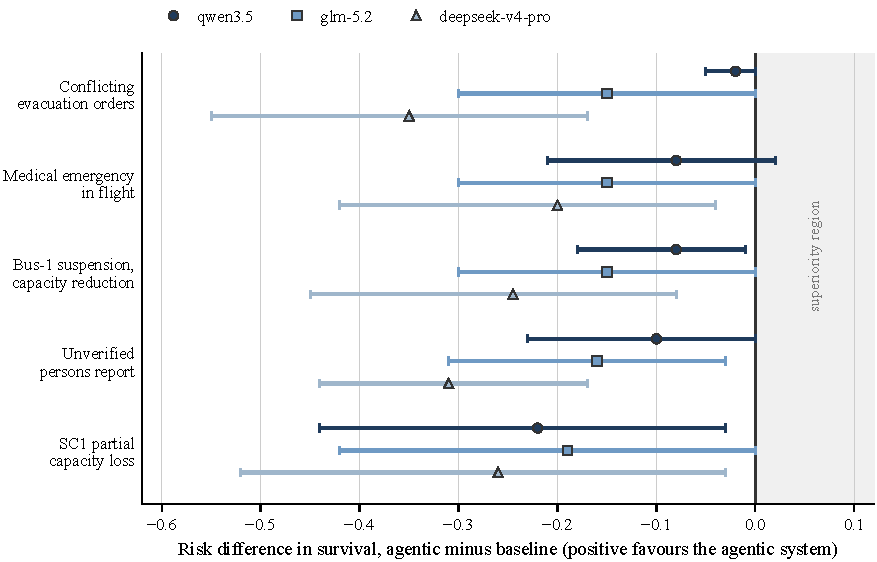
\includegraphics[width=\textwidth]{pics/results-forest-rd.pdf}
\caption[Novel-arm risk differences]{The 15 novel-arm risk differences with
their bootstrap confidence intervals. A superiority result would need the whole
interval to sit inside the shaded region. None does, and no point estimate is
positive. Table~\ref{tab:res:rd} gives the same values exactly. Drawn from
\texttt{data/novel\_risk\_differences.csv}.}
\label{fig:res:forest}
\end{figure}

Superiority needs the paired interval to exclude zero on the positive side. No
cell comes close. Every point estimate is negative.
Figure~\ref{fig:res:forest} shows why the verdict does not depend on reading
any single row. All 15 intervals lie to the left of zero. Eight stay strictly
below it, six reach zero and stop there, and exactly one reaches past it:
qwen3.5 on
\code{medical_emergency_in_flight}, whose upper bound is 0.02. The three models
also separate cleanly in the figure, which is the capability ordering that
Section~\ref{sec:res:models} returns to.

\subsection{The H2 Minimum Effect}
\label{sec:res:novel:delta}

H2 also set a minimum effect. It required a median shift of one whole recovery
level, $\delta_m = +1.0$, together with first-order stochastic dominance of the
agentic system over the baseline. Table~\ref{tab:res:levelshift} gives the
median paired level shift in each cell.

\begin{table}[htbp]
\centering
\caption{Median paired level shift, agentic minus baseline. The registered
minimum effect was $+1.0$.}
\label{tab:res:levelshift}
\small
\begin{tabular}{lccc}
\toprule
Disruption & qwen3.5 & glm-5.2 & deepseek \\
\midrule
\code{conflicting_evacuation_orders} & 0.0 & 0.0 & $-2.0$ \\
\code{medical_emergency_in_flight} & 0.0 & 0.0 & $-2.0$ \\
\code{unverified_persons_report} & 0.0 & $-0.5$ & $-2.0$ \\
\code{bus1_suspension_capacity_reduction} & $-0.5$ & $-0.5$ & $-2.0$ \\
\code{sc1_partial_capacity_loss} & $-1.0$ & 0.0 & 0.0 \\
\bottomrule
\end{tabular}
\end{table}

No cell is positive. Every novel row reads \code{below_delta_m} with
dominance assigned to the baseline, so neither of the two conditions holds
anywhere. The best the agentic system manages is parity of median level on four
of the five disruptions, and it reaches that parity while still losing
residents. That is exactly why Gate~1 fails where the median level does not.

\subsection{The Registered H2 Primary}
\label{sec:res:novel:prereg}

The pre-registration named a different primary test for H2. It registered an
exact Clopper-Pearson interval on $P(\text{level}_{\text{agentic}} \geq
\text{level}_{\text{baseline}})$ over the $k$ agentic runs against the
control's constant level, aggregated across scenarios by a sign test with
Holm-Bonferroni correction.

\textbf{That test was not implemented when the results above were first
written.} It was coded afterwards, once the result was already known. This is a
deviation from the pre-registration's timing and is reported as one. Under the
pre-registration's own rules the analysis is therefore exploratory.
Chapter~\ref{ch:critique} treats it properly. The numbers are given here
because they belong beside the verdict they check.

The control scored level 4 on all 50 novel runs, so the success event is that
the agentic run also reached level 4.

\begin{table}[htbp]
\centering
\caption{Registered H2 primary: successes out of 10 with exact
Clopper-Pearson intervals.}
\label{tab:res:cp}
\footnotesize
\begin{tabular}{lccc}
\toprule
Disruption & qwen3.5 & glm-5.2 & deepseek \\
\midrule
\code{conflicting_evacuation_orders} & 7/10 [0.35, 0.93] & 7/10 [0.35, 0.93] & 1/10 [0.00, 0.44] \\
\code{medical_emergency_in_flight} & 7/10 [0.35, 0.93] & 7/10 [0.35, 0.93] & 4/10 [0.12, 0.74] \\
\code{sc1_partial_capacity_loss} & 5/10 [0.19, 0.81] & 7/10 [0.35, 0.93] & 6/10 [0.26, 0.88] \\
\code{unverified_persons_report} & 6/10 [0.26, 0.88] & 5/10 [0.19, 0.81] & 2/10 [0.03, 0.56] \\
\code{bus1_suspension_capacity_reduction} & 5/10 [0.19, 0.81] & 5/10 [0.19, 0.81] & 2/10 [0.03, 0.56] \\
\bottomrule
\end{tabular}
\end{table}

The registered test agrees with the risk-difference verdict. Not one cell puts
the agentic system above chance. No interval has a lower bound above 0.5. One
cell sits below chance before correction, deepseek on
\code{conflicting_evacuation_orders} at 1 of 10 with $p = 0.021$, and it
does not survive the Holm correction, where $p = 0.107$.

The aggregation across scenarios is reported in Table~\ref{tab:res:signtest},
with one observation per scenario, because the pre-registration forbids pooling
runs across scenarios.

\begin{table}[htbp]
\centering
\caption{Registered scenario-level sign test. The last column is the smallest
$p$ the design could have produced for that model.}
\label{tab:res:signtest}
\small
\begin{tabular}{lcccccc}
\toprule
Model & scenarios & favour agentic & favour baseline & ties & $p$ & floor on $p$ \\
\midrule
qwen3.5 & 5 & 3 & 0 & 2 & 0.250 & \textbf{0.250} \\
glm-5.2 & 5 & 3 & 0 & 2 & 0.250 & \textbf{0.250} \\
deepseek-v4-pro & 5 & 1 & 4 & 0 & 0.375 & 0.0625 \\
\bottomrule
\end{tabular}
\end{table}

There is a second finding in that table, and it is about the design rather than
the systems. \textbf{At $k = 10$ this test can hardly conclude anything.} Every
Clopper-Pearson interval is about 0.6 wide, so even a cell at 7 of 10 cannot
separate from chance. The sign test is worse. A two-sided exact sign test on
five scenarios cannot return a $p$ below 0.0625 however the data fall, and ties
push the floor higher. qwen3.5 and glm-5.2 each tie two scenarios, which leaves
three untied observations and a floor of 0.250. Both models are therefore
already sitting at the smallest $p$ their data could have produced. The
registered aggregation cannot reach conventional significance in this design at
all.

This is why the risk difference carries the argument. It is continuous, it is
paired, and it is far more efficient with the replicates available. The
weakness of the registered plan is a limitation of the analysis plan, not a
result, and Chapter~\ref{ch:critique} takes it up as a methods finding.

One more warning about Table~\ref{tab:res:signtest}. The sign test's direction
is mildly favourable to qwen3.5 and glm-5.2, with three scenarios above chance,
none below and two tied, while both models still lose residents in every cell.
That is not a win. The sign test counts which side of 0.5 a cell falls on and
is blind to how far, which is precisely the information the risk difference
keeps.

\subsection{What the Novel Arm Does Not Show}
\label{sec:res:novel:boundary}

The novel arm answers whether the agentic system won on these scenarios. It
does not answer whether an agentic system can ever win, because no scenario in
this thesis ever \emph{required} adaptation. Chapter~\ref{ch:critique} shows
that a controller which ignores every disruption scores the same level as the
baseline on all five novel scenarios. The baseline's $S$ of 1.000 is the null
policy's score.

Two consequences follow, and both hold for every table in this chapter. First,
the baseline's result must never be described as recovery, adaptation or better
replanning. It did not adapt, because nothing it did changed an order or a
kilometre. Second, that withdrawal cuts one way only. It does not turn into an
agentic win. Against the same null policy the agentic regret is negative in all
15 novel cells, and 68 of 150 runs came out worse than doing nothing at all.

\section{What the Losses Were Made Of}
\label{sec:res:loss}

The survival tables say how much was lost. This section says what the loss was
made of, because the shape of the loss is what Chapter~\ref{ch:discussion}
builds on.

\subsection{Residents Never Moved}
\label{sec:res:loss:nevermoved}

\begin{table}[htbp]
\centering
\caption{Residents never moved, per 100. Lower is better.}
\label{tab:res:nevermoved}
\small
\begin{tabular}{lcccc}
\toprule
Disruption & baseline & qwen3.5 & glm-5.2 & deepseek \\
\midrule
\code{medical_emergency_in_flight} & 0.0 & \textbf{5.0} & 10.0 & 13.0 \\
\code{conflicting_evacuation_orders} & 0.0 & \textbf{2.0} & 15.0 & 19.0 \\
\code{bus1_suspension_capacity_reduction} & 0.0 & \textbf{2.0} & 15.0 & 22.5 \\
\code{unverified_persons_report} & 0.0 & \textbf{4.0} & 10.0 & 21.0 \\
\code{sc1_partial_capacity_loss} & 0.0 & \textbf{2.5} & 14.0 & 16.0 \\
\bottomrule
\end{tabular}
\end{table}

qwen3.5 strands far fewer residents than the other two models. It does so on
every disruption, by a factor of two to eight. Its survival deficit comes
mostly from residents arriving late or being invalidated by shelter overload,
not from residents left behind. That is a materially different failure from
deepseek's, and Section~\ref{sec:res:models} returns to it.

These figures were corrected after the first write-up. The column was computed
as the ceiling minus sheltered residents with no floor at zero, and the
over-delivery runs of Section~\ref{sec:res:integrity} drove two cells negative.
It is now floored at zero. Five cells changed. No confirmatory number moved.

\subsection{Late Arrivals and Shelter Overload}
\label{sec:res:loss:totals}

The two recorded loss mechanisms are residents who missed their deadline and
residents invalidated because a shelter was filled past what it declared.
Table~\ref{tab:res:lossmech} gives the totals. The scope has to be stated with
them, because the figures differ by nearly a factor of two depending on which
runs are counted.

\begin{table}[htbp]
\centering
\caption{Loss mechanism totals by scope.}
\label{tab:res:lossmech}
\small
\begin{tabular}{lccc}
\toprule
Scope & late arrivals & in runs & shelter-overload invalidations \\
\midrule
All agentic runs, both arms, all 7 models & 1\,675 & 41 & 215 \\
Agentic novel arm only & 1\,035 & 28 & 215 \\
Agentic novel arm, 3 full models only & 985 & 26 & 215 \\
\textbf{baseline, all runs} & \textbf{0} & \textbf{0} & \textbf{0} \\
\bottomrule
\end{tabular}
\end{table}

The figure of 1\,675 includes minimax-m3 and nemotron-3-ultra, and neither
model is part of the headline result. A novel-arm claim should quote the
novel-arm figure. The baseline recorded no late arrival and no overload in any
run.

\subsection{The Loss Is Not a Message-Layer Failure}
\label{sec:res:loss:handshakes}

An early reading of these results attributed the deficit to unanswered
handshakes. Measurement does not support that reading. Over 1\,932 addressed
requests in the agentic novel arm, handshake closure is \textbf{0.938}. The
three highest-volume handshakes close at 0.947, 0.970 and 0.997. The one weak
handshake is \code{abort_request} at 0.548, and it sits on a small
denominator of 31 requests.

The dominant mechanism is residents who were never dispatched at all. Across
the 150 agentic novel runs from the three full models, the correlation of
never-dispatched residents with $S$ is $r = -0.745$, against $-0.579$ for late
arrivals and $+0.061$ for shelter overload. The failure is in what the agents
committed to move, not in whether their messages arrived.

These are exploratory Protocol~v2 instruments, written after the data were
seen. They change no confirmatory number. Chapter~\ref{ch:critique} reports
them in full, together with the alternative explanations that were ruled out.

\subsection{The Loss Is Quantised}
\label{sec:res:loss:quantised}

Figure~\ref{fig:res:delivery} gives the distribution of residents delivered
across the same 150 runs. The shape is the argument.

\begin{figure}[htbp]
\centering
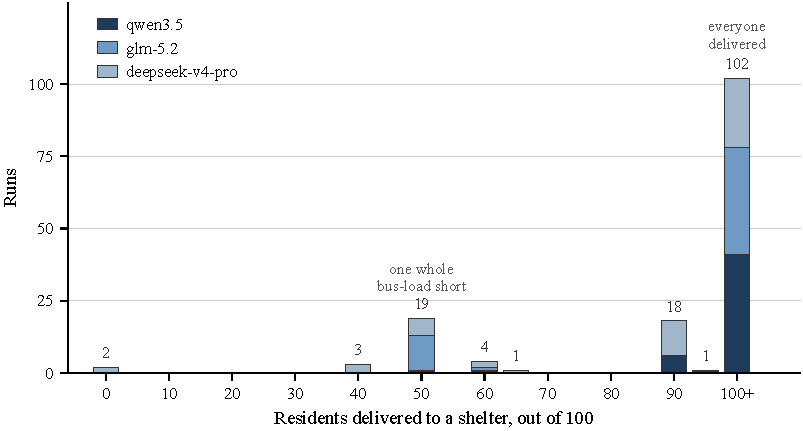
\includegraphics[width=\textwidth]{pics/results-delivery-histogram.pdf}
\caption[Residents delivered per run]{Residents delivered to a shelter, over
the 150 agentic novel runs from the three full models. The distribution
clusters on a few discrete values instead of spreading smoothly. The six runs
that report more arrivals than the ceiling admits
(Section~\ref{sec:res:integrity}) are folded into the \mbox{100+} column, the
same way the survival tables cap them. Drawn from
\texttt{data/delivery\_distribution.csv}.}
\label{fig:res:delivery}
\end{figure}

Of the 150 runs, 102 delivered everyone. Nineteen delivered exactly 50, which
is one whole bus-load short. Eighteen delivered exactly 90, and two delivered
nobody at all. Nothing lands between 65 and 90, and nothing lands between 10
and 40.

A system degrading under load does not produce that picture. It produces a
spread. A system that loses discrete committed legs does produce it. Together
with the 0.938 handshake closure, this is what moves the diagnosis from
comprehension to commitment: the agents understood the disruption and were
heard, and then failed to carry a plan they had already committed to through to
the end.

The figure also separates the models. The spike at 50 is mostly glm-5.2, with
12 of its 19 runs. The spike at 90 is mostly deepseek-v4-pro, with 12 of 18.
qwen3.5 holds 41 of the 102 full deliveries. This is descriptive and
exploratory, and Chapter~\ref{ch:critique} carries the causal argument and its
limits.

\section{Decision Quality}
\label{sec:res:quality}

Decision quality was measured by a held-out rubric applied to the novel arm.
The rubric is a secondary, structural measure. It is never tabulated beside a
recovery level, and it does not enter any gate. Each cell counts \texttt{yes}
judgements out of 10. A cell short of 10 had the remainder judged \texttt{no}
or \texttt{unanswerable}.

Table~\ref{tab:res:rubric} gives all five novel disruptions and all sixteen
criteria.

% TODO(figure): the 16-criteria split drawn as three bands (parity on 5,
% baseline wins 5, scenario-indicting 3). Source: RESULTS.md sec. 4.

\begin{table}[htbp]
\centering
\caption{Held-out decision rubric, \texttt{yes} judgements out of 10.}
\label{tab:res:rubric}
\footnotesize
\begin{tabular}{lcccc}
\toprule
Criterion & baseline & qwen3.5 & glm-5.2 & deepseek \\
\midrule
\multicolumn{5}{l}{\emph{Disruption:} \code{bus1_suspension_capacity_reduction}} \\
\quad \code{reserve_committed} & 10 & \textbf{10} & \textbf{10} & 9 \\
\quad \code{whole_population_planned} & 10 & \textbf{10} & \textbf{10} & 6 \\
\quad \code{bus_load_within_cap} & 0 & 0 & 3 & 2 \\
\midrule
\multicolumn{5}{l}{\emph{Disruption:} \code{conflicting_evacuation_orders}} \\
\quad \code{authority_informed} & 10 & \textbf{10} & 9 & \textbf{10} \\
\quad \code{full_evacuation_kept} & 10 & 9 & \textbf{10} & 5 \\
\quad \code{facility_answered_in_time} & \textbf{10} & 0 & 0 & 0 \\
\midrule
\multicolumn{5}{l}{\emph{Disruption:} \code{medical_emergency_in_flight}} \\
\quad \code{authority_informed} & 10 & \textbf{10} & \textbf{10} & \textbf{10} \\
\quad \code{in_flight_leg_lands_where_ordered} & 10 & 8 & 6 & 6 \\
\quad \code{medic_sent_to_the_bus_destination} & 0 & 1 & 1 & 0 \\
\midrule
\multicolumn{5}{l}{\emph{Disruption:} \code{unverified_persons_report}} \\
\quad \code{verification_requested} & 10 & 9 & \textbf{10} & \textbf{10} \\
\quad \code{stood_down_after_retraction} & 10 & \textbf{10} & \textbf{10} & 8 \\
\quad \code{reserve_committed_in_time} & 10 & 9 & \textbf{10} & 9 \\
\quad \code{facility_runs_untouched} & \textbf{10} & 7 & 8 & 5 \\
\midrule
\multicolumn{5}{l}{\emph{Disruption:} \code{sc1_partial_capacity_loss}} \\
\quad \code{no_order_raises_shelter_above_beds} & \textbf{10} & 5 & 9 & 8 \\
\quad \code{shelter_set_down_within_beds} & 0 & 2 & 2 & 0 \\
\quad \code{everyone_bedded_at_the_reduced_capacity} & 0 & 0 & 0 & 0 \\
\bottomrule
\end{tabular}
\end{table}

Read across all sixteen criteria, the rubric splits three ways.

\begin{sloppypar}
\textbf{Parity on five criteria.} These are \code{authority_informed} on both
disruptions, \code{reserve_committed}, \code{whole_population_planned} and
\code{stood_down_after_retraction}. qwen3.5 and glm-5.2 match the baseline's 10
out of 10 on all of them. This is the evidence that the agents reason about the
disruption correctly.

\textbf{The baseline wins on five criteria.} The clearest is
\code{facility_answered_in_time}, where the baseline scores 10 and no agentic
model ever answered the facility in time. The others are
\code{no_order_raises_shelter_above_beds} at 10 against 5, 9 and 8,
\code{facility_runs_untouched} at 10 against 7, 8 and 5,
\code{in_flight_leg_lands_where_ordered} at 10 against 8, 6 and 6, and
\code{full_evacuation_kept} at 10 against 9, 10 and 5.
\end{sloppypar}

\textbf{Three criteria indict the scenario rather than either architecture.}
\code{bus_load_within_cap},
\code{medic_sent_to_the_bus_destination} and
\code{everyone_bedded_at_the_reduced_capacity} score 0 for the baseline
too. They cannot be reported as agentic failures. On
\code{shelter_set_down_within_beds} the agentic side actually beats the
baseline, at 2 and 2 against 0.

\textbf{Decision quality is split, not at parity.} Over the sixteen criteria
the agentic models match the baseline on five and fall short on five. Parity
holds on the criteria about deciding, and fails on the criteria about closing
the loop. This chapter does not round that to decision-quality parity, and
neither does any later chapter.

\section{Response Time and Cost}
\label{sec:res:responsetime}

The baseline's model latency is 0.0 seconds by construction, because it runs no
model at all. Agentic wall-clock latency per run ranges from 763 seconds for
deepseek on \code{closed_loop} to 3\,810 seconds for kimi-k3 on
\code{medical_emergency_in_flight}. Within the three full novel arms the
per-cell means sit between 815 seconds, for deepseek on
\code{unverified_persons_report}, and 2\,528 seconds, for glm-5.2 on
\code{bus1_suspension_capacity_reduction}.

Bus kilometres are comparable only within a system, not between the two,
because the systems compose the total differently. The baseline drove 60.63
bus-km on every novel scenario, and the same 60.63 undisrupted. That single
fact is one of the reasons Chapter~\ref{ch:critique} exists.

The coordination surface is the cost that the original protocol never printed.
Table~\ref{tab:res:surface} gives it for the 150 agentic novel runs and their
50 paired control runs. These are exploratory Protocol~v2 figures.

\begin{table}[htbp]
\centering
\caption{Coordination surface on the novel arm. Exploratory.}
\label{tab:res:surface}
\footnotesize
\begin{tabular}{lcccccc}
\toprule
System and model & nodes & messages & decisions & msgs / resident & tokens & budget fraction \\
\midrule
baseline & 2 & 13.2 & 13.2 & \textbf{0.13} & 0 & 0.00 \\
agentic / deepseek-v4-pro & 11 & 91.9 & 152.6 & 1.26 & 725\,457 & 1.80 \\
agentic / qwen3.5 & 11 & 106.6 & 170.3 & 1.18 & 894\,243 & 2.28 \\
agentic / glm-5.2 & 11 & 111.8 & 174.9 & 1.33 & 829\,906 & 2.70 \\
\bottomrule
\end{tabular}
\end{table}

The control coordinates a hundred-resident evacuation on 13 messages into one
node. The agentic system spends seven to eight and a half times as many
messages across eleven nodes, which is nine to ten times as many per resident
delivered. It also spends roughly 800\,000 tokens and 1.8 to 2.7 times the
wall-clock that the compressed clock allows. 140 of the 150 runs finished over
budget.

On these scenarios that surface bought nothing. Whether it buys anything on a
scenario that actually requires adaptation is an open question, and this design
cannot answer it.

\section{Process Diagnostics}
\label{sec:res:diagnostics}

Process diagnostics explain the outcome distribution. They do not score it.
Supersede count in particular rewards churn, and the protocol demotes it on
purpose.

The diagnostic that turned out to matter is the number of plan revisions.
Table~\ref{tab:res:commitment} bands the 150 agentic novel runs by it.

% TODO(figure): plan revisions against full-delivery rate, 90 % down to 32 %.
% Source: EVALUATION_PROTOCOL_V2.md sec. 11.4.

\begin{table}[htbp]
\centering
\caption{Plan revisions against delivery, 150 agentic novel runs.
Exploratory.}
\label{tab:res:commitment}
\small
\begin{tabular}{lcccc}
\toprule
Plan revisions & runs & mean $S$ & mean aborts & full delivery \\
\midrule
2 (the minimum) & 61 & 0.923 & 0.08 & \textbf{90\%} \\
3 & 22 & 0.827 & 0.55 & 77\% \\
4 & 15 & 0.853 & 0.67 & 67\% \\
5 & 11 & 0.782 & 1.27 & 64\% \\
6 or more & 41 & 0.670 & 1.63 & \textbf{32\%} \\
\bottomrule
\end{tabular}
\end{table}

The full-delivery rate falls monotonically across the bands, from 90\% at the
minimum revision count to 32\% at six or more. The correlation of plan
revisions with $S$ is $r = -0.408$, which is the strongest non-definitional
predictor in the data. Aborts correlate at $r = -0.306$. The number of missions
dispatched correlates at only $r = -0.070$, so it is not how many missions were
ordered but how many times the plan was rewritten.

The causal direction is not established, and this chapter does not claim it. Of
108 aborts, 52.8\% are explicit post-failure stand-downs and only 13.0\% are
clearly revision-initiated. A run that is going badly plausibly re-plans because
it is going badly. Observational data cannot separate the two directions.
Chapter~\ref{ch:critique} names the experiment that would.

\section{Model Sweep and Capability Threshold}
\label{sec:res:models}

The gap narrows with model capability. The mean novel-arm risk difference is
$-0.27$ for deepseek-v4-pro, $-0.16$ for glm-5.2 and $-0.10$ for qwen3.5. The
ordering is consistent across all five novel disruptions. On four of the five,
qwen3.5 matches the baseline's median level while still losing residents, so it
reaches the same recovery category without the same survival.

The weaker models fail badly rather than narrowly. minimax-m3 scored 0.340 on
\code{closed_loop} and 0.150 on \code{road_closure}. nemotron-3-ultra
scored 0.000 on the two runs it completed. Neither model is part of the
headline result.

No capability threshold is observable inside the final model set, and the
design does not support extrapolating past qwen3.5.

\textbf{Hypothesis H3 cannot be resolved, because it presupposes H2.} H3
predicted that the agentic advantage on novel disruptions would be
model-robust, with a capability threshold below which that advantage
disappears. There is no advantage here to be robust or fragile. The threshold
H3 asks about is therefore undefined rather than unobserved, and no verdict on
H3 is reported. What the model sweep does establish is the ordering above: the
size of the deficit tracks model capability, consistently, across every novel
disruption. That is a descriptive finding and not the registered hypothesis.

\subsection{Why Levels Are Comparable for Three Arms Only}
\label{sec:res:models:levelcap}

A promotion to level 4 requires a resource-efficiency judgement against the
model's own no-disruption reference. That reference needs three qualifying
control runs. A model with no \code{agentic_closed_loop} runs is capped at
level 3 regardless of how well it performed.

qwen3.5 was originally novel-arm-only and was capped by this rule. It held the
best agentic survival with zero level-4 runs, which made every level-based
comparison involving it an artifact. Amendment~13 ran its ten anticipated
\code{closed_loop} cells to supply the reference. After re-scoring it has 30
level-4 runs and a median level of 4, against glm-5.2's 31 and 4. Levels are
now comparable across the three full arms.

Three series remain capped and are comparable on $S$ only. These are kimi-k3
with 11 runs at $S = 0.773$, kimi-k2.7-code with 3 runs at 0.667 and gpt-oss
with 4 runs at 0.375. They must never be ranked by level against the full arms.

Re-scoring changed no survival figure. $S$, $RD$ and Gate~1 are computed per
run and never consult the clean-run reference. The Gate~1 verdicts before and
after re-scoring are identical.

\subsection{The Third Model Slot Changed Four Times}
\label{sec:res:models:churn}

The novel arm's third model slot was held in turn by kimi-k3 with 11 runs,
gpt-oss with 4, kimi-k2.7-code with 3 and finally qwen3.5 with 50. Each swap
was made after seeing data. Under the pre-registration the novel arm's model
set, and any analysis using it, is therefore exploratory. The four short series
are reported separately and never pooled. glm-5.2 and deepseek-v4-pro were
fixed before the novel arm ran and are unaffected.

\section{Sensitivity Analysis}
\label{sec:res:sensitivity}

The protocol makes the cut-point sensitivity analysis a precondition on the
headline. Each cell's median level was re-read with the level 1 to 2 cut moved
to 0.40, 0.50 and 0.60. A cell is stable when it reads the same at all three
cuts.

\textbf{The result supports the headline.} Every cell in the three full novel
arms reads the same median at all three cuts, with one exception:
\code{unverified_persons_report} for deepseek moves from 2.0 to 1.5 at the
0.60 cut. The only other unstable cells are minimax-m3 on the anticipated arm
and two partial series, kimi-k2.7-code at $n = 3$ and kimi-k3 at $n = 1$. No
agentic-versus-baseline ordering moves anywhere in the cut range.

This analysis was also missing from the first write-up. The summary asserted
that it had to be reported but printed no table, and the reporting script never
read the field. It is now aggregated and emitted.

\section{Integrity of the Reported Numbers}
\label{sec:res:integrity}

Two defects in the measurement are visible in the tables above. Both are
reported here rather than corrected in the scorer, because correcting them
after the fact would rewrite a confirmatory result.

\subsection{Six Runs Shelter More Residents Than the Ceiling Admits}
\label{sec:res:integrity:ceiling}

Three qwen3.5 runs score $S = 1.1$. The visible symptom is an impossible
survival value. Table~\ref{tab:res:overceiling} shows that the defect is wider
than those three runs.

\begin{table}[htbp]
\centering
\caption{Runs reporting sheltered residents above the feasibility ceiling.}
\label{tab:res:overceiling}
\footnotesize
\begin{tabular}{lllcccc}
\toprule
Run & Model & Disruption & sheltered & ceiling & valid & $S$ \\
\midrule
\texttt{03459286} & qwen3.5 & \code{medical_emergency_in_flight} & 150 & 100 & 110 & \textbf{1.10} \\
\texttt{d66ce694} & qwen3.5 & \code{unverified_persons_report} & 150 & 100 & 110 & \textbf{1.10} \\
\texttt{8bd769f8} & qwen3.5 & \code{sc1_partial_capacity_loss} & 150 & 100 & 110 & \textbf{1.10} \\
\texttt{eb997b3e} & qwen3.5 & \code{sc1_partial_capacity_loss} & 150 & 100 & 100 & 1.00 \\
\texttt{ca9bdde5} & deepseek & \code{bus1_suspension} & 115 & 100 & 100 & 1.00 \\
\texttt{5961b028} & deepseek & \code{medical_emergency_in_flight} & 130 & 100 & 90 & 0.90 \\
\bottomrule
\end{tabular}
\end{table}

Three of the six are masked, because their valid-resident count stayed at or
below the ceiling and $S$ therefore looks ordinary. Reporting only the subset
with $S > 1.0$ would understate the problem.

The mechanism is now diagnosed, and it is not a double count. The feasibility
ceiling is the smaller of the population and the total declared beds, so it is
capped at 100 by the population. Valid residents are capped only by per-shelter
beds. Sheltered residents are a raw sum over logged arrivals and are capped by
nothing. Where two shelters declare 110 beds between them, a run can validly
shelter 110 against a ceiling of 100. So this is genuine over-delivery credited
against a ceiling that does not admit it, not a logging artifact.

The cap stays at the reporting layer, where it is visible and stated. Capping
at 1.0 moves qwen3.5's novel mean from 0.900 to 0.894 and changes no
conclusion. A value of $S$ above 1.0 does not appear in any table in this
thesis.

One further inconsistency is undiagnosed. Run \texttt{eb997b3e} shelters 150
against a ceiling of 100 with its overload count recorded as 0, so the overload
accounting does not agree with the arrival sum on that run.

\subsection{Standing Caveats}
\label{sec:res:integrity:caveats}

The following apply to every table in this chapter. They are listed in full,
with the position taken on each, in Chapter~\ref{ch:critique}.

\begin{itemize}
\item \textbf{One time scale, so H4 was not tested.}
  \label{sec:res:h4}
  The scenario-scaling sweep was planned and never run. Every result in this
  chapter is at a single \code{SIM_TIME_SCALE} of 8.4, so Gate~3's adaptability
  series has one point per cell and no crossover can be located. H4 asked at
  which time scale the agentic latency cost overtakes its coordination benefit.
  This chapter reports no crossover, no trend and no scale-dependence claim of
  any kind. The evaluation is finished, so this is permanent rather than
  pending.
\item \textbf{Reserve-bus confound.} The baseline parallelises the reserve bus
  while the agentic side honours the reserve role and serialises it. This
  drives part of the gap. It is architectural, not a model effect.
\item \textbf{One run flagged for possible straight-line routing},
  \texttt{aaae313d}, during a routing-service quota outage.
\item \textbf{Equity is undefined by declaration.} The resident population is
  homogeneous, so a maximum-minimum subgroup difference is identically zero.
\item \textbf{Cloud model tags are not version-frozen.} The serving runtime
  resolves whatever a tag currently points at, and no digest pins these
  results.
\item \textbf{Two parity deviations favour the baseline}, the consolidated
  situation picture and the controller's access to road distance and duration.
  Both were accepted for doctrinal reasons and reported rather than corrected.
\item \textbf{One parity deviation was still open when the campaign ran.} Its
  direction runs against the baseline, so it cannot explain a baseline win.
  Chapter~\ref{ch:validity} carries that argument.
\end{itemize}

\section{Summary of Findings}
\label{sec:res:findings}

\begin{enumerate}
\item The workflow baseline is superior on survival across all seven scenarios.
  Gate~1 fails in 26 of 27 cells. \textbf{H1 is rejected}: non-inferiority
  holds in 1 of 8 anticipated cells and fails in the other 7.
\item \textbf{H2 is rejected outright}, on both of its co-primaries. Zero of 19
  novel Gate~1 cells pass on survival, and no cell reaches the registered
  minimum effect of one recovery level. The registered Clopper-Pearson primary,
  implemented late and therefore exploratory, agrees with that verdict. It also
  could not have detected a moderate effect at $k = 10$.
\item \textbf{H3 cannot be resolved}, because it presupposes the advantage H2
  failed to establish. The capability threshold it asks about is undefined
  rather than unobserved. What the model sweep does show is that the size of
  the deficit narrows with model capability, from $-0.27$ for deepseek through
  $-0.16$ for glm-5.2 to $-0.10$ for qwen3.5, consistently across all five
  novel disruptions. That is descriptive. Extrapolating past qwen3.5 is not
  supported by this design.
\item Agentic non-inferiority holds in exactly one place, glm-5.2 on the
  undisrupted \code{closed_loop}.
\item Decision quality is split. Over the sixteen rubric criteria the agentic
  models match the baseline on five and fall short on five.
\item \textbf{H4 was not tested.} Only one time scale was run.
\end{enumerate}

The baseline's win is not evidence that it adapted, and the agentic loss is not
a failure of comprehension. Chapter~\ref{ch:critique} establishes the first,
and Chapter~\ref{ch:discussion} argues the second.


% The methods critique reads the results back against the protocol. It follows
% the results because it depends on them.
\chapter{Methods Critique}
\label{ch:critique}

% SOURCE OF TRUTH: thesis-pack/09-method/EVALUATION_PROTOCOL_V2.md
% (= PREREGISTRATION Amendment 16, 2026-09-22), plus RESULTS sec.6.7 and 6.8,
% the Gate 0 evidence in thesis-pack/11-results/data/discrimination-*.md, and
% the v2 instruments in thesis-pack/11-results/data/v2.md.
%
% TONE RULE. No hedging and no self-flagellation. State the defect, state the
% evidence, state the gate that catches it, state what stands.

This chapter reads the results back against the protocol that produced them.
It exists because the protocol, applied to its own data, found that its primary
arm could not have answered the question it was built for. That finding is
reported here as a result in its own right. A protocol that detects a
degenerate treatment with its own negative control, and then specifies the gate
that would have caught it, has done its job.

The chapter does not repeat the numbers of Chapter~\ref{ch:results}. It points
to them and adds only what is new: the treatment-validity gate and its
evidence, the regret against a null policy, the alternative explanations that
were ruled out, and the position taken on each declared limitation.

Everything in Sections~\ref{sec:crit:gate0} to~\ref{sec:crit:mechanism} was
designed after the evaluation data had been seen. It is registered as
Protocol~v2 in Amendment~16, and under the pre-registration's own rules it is
exploratory without exception. It changes the \emph{name} of what the first
protocol measured. It does not change a single number, and it does not change
the sign of the result.

One boundary holds for the whole chapter. No scenario in this thesis ever
\emph{required} adaptation. RQ1 is therefore answered as ``did the agentic
architecture win here'', not ``can it ever win''.

% =====================================================================
\section{The Defect}
\label{sec:crit:defect}

The novel arm was built to test H2: does the agentic system recover better than
a scripted workflow when a disruption arrives that the workflow has no branch
for? On that arm the workflow baseline scored $S = 1.000$ in all 50 of its
runs. That perfect score is not a recovery. It is an \emph{invariance}, and the
scenario design guaranteed it before any model was chosen.

The reason is in how the scenarios are written. Every event in every one of the
fourteen scenario files is an envelope of the form \texttt{\{at, send\}}: at a
given time, send a given message. No scenario event changes the declared world
state, that is the \code{world}, \code{sensing} or \code{hazard} blocks. The
disruption exists as text in an inbox and nowhere else. When SC1 reports a
partial capacity loss, SC1 keeps declaring 60 beds. When bus-1 is suspended,
bus-1 keeps its seats.

So the baseline's physical plan is not touched by the disruption. It drives
60.63 bus-km on the undisrupted \code{closed_loop} and 60.63 bus-km on each of
the five novel disruptions (Section~\ref{sec:res:responsetime}). Not one
kilometre moves.

The protocol's own negative control confirms this. The no-replan control of
Section~\ref{sec:eval:noreplan} is the doctrine baseline with re-planning
switched off, so it ignores every disruption. Run against the scored scenarios,
it commits byte-identical orders and scores the identical level on all five
novel files and on \code{closed_loop}.

On the novel arm, then, \textbf{ignoring the disruption is an optimal policy}.
A test in which doing nothing scores at the ceiling cannot produce evidence for
or against an adaptability hypothesis, in either direction. The agentic
system's only route to a non-negative risk difference was to also do nothing,
and doing nothing is exactly what an agentic architecture is built not to do.

The first protocol knew the mechanism and wrote it down. As
Section~\ref{sec:eval:noreplan} quotes, it stated that on every scored scenario
the control ``cannot differ from the doctrine in outcome, by construction''.
It used that note as the reason to read the negative control on a separate
fixture. The error was not concealment. The error was that the gate's guarantee
was never required to hold on the files where the hypotheses were actually
read.

% =====================================================================
\section{Gate 0: Treatment Validity}
\label{sec:crit:gate0}

Protocol~v2 adds a gate that is read before Gates 1 to 3, and read per
scenario rather than per system:

\begin{quote}
A scenario is admitted to a confirmatory adaptability arm only if a system
that ignores its disruption scores strictly worse on it than one that
responds.
\end{quote}

A scenario that fails Gate~0 may still be run and reported. It is then a
legitimate test of \emph{base execution}. But it may not carry an adaptability
claim, and no risk difference computed on it may be described as evidence about
re-planning. The gate is cheap. It costs two runs of the control per scenario
and reuses the no-replan machinery the first protocol already built.

A disruption is \emph{binding} when three conditions hold. Each one isolates a
different way a scenario can fail to test what it was written to test.

\begin{description}
\item[D1, state-mutating.] The disruption changes declared world state, not
  only an inbox. A purely informational disruption can still bind in principle,
  if acting on the information is required to succeed. But this cannot be
  assumed.
\item[D2, order-binding.] The null policy does not commit the same order
  sequence as the responding policy. If the orders are byte-identical, no
  downstream instrument can tell the two apart, whatever it measures.
\item[D3, outcome-binding.] The null policy scores a strictly lower outcome.
  D2 without D3 means the plans really differ, but the scoring function cannot
  see it.
\end{description}

A fourth condition applies to the scenario \emph{set}, not to each scenario.
\textbf{D4, recoverable:} at least one policy must reach the feasibility
ceiling. A disruption that no policy can recover from measures the hazard, not
the coordinator.

Table~\ref{tab:crit:gate0} is the evidence. It runs the doctrine baseline and
the no-replan control side by side on the fixture and on all seven scored
scenarios. Both variants are scored without a clean-run reference, so both are
capped at level 3. The comparison is between the two variants, not against the
campaign's level 4.

\begin{table}[htbp]
\centering
\caption[Gate 0 evidence: the no-replan control on the scored scenarios]{Gate~0
evidence. The doctrine baseline against the no-replan control, which ignores
every disruption. $L$ is the level, capped at 3 here, with completeness in
brackets. Only the fixture discriminates. Exploratory.}
\label{tab:crit:gate0}
\scriptsize
\setlength{\tabcolsep}{3.5pt}
\begin{tabular}{lccccccc}
\toprule
 & & orders & \multicolumn{2}{c}{level $L$ (C)} & \multicolumn{2}{c}{bus-km} & discri- \\
\cmidrule(lr){4-5}\cmidrule(lr){6-7}
Scenario & world & identical & doctrine & no-replan & doctrine & no-replan & minates \\
\midrule
\emph{fixture:} \code{shelter_closure} & yes & no & 3 (1.0) & 0 (0.0) & 83.12 & 38.14 & \textbf{yes} \\
\midrule
\code{medical_emergency_in_flight} & yes & yes & 3 (1.0) & 3 (1.0) & 60.63 & 60.63 & no \\
\code{unverified_persons_report} & yes & yes & 3 (1.0) & 3 (1.0) & 60.63 & 60.63 & no \\
\code{conflicting_evacuation_orders} & yes & yes & 3 (1.0) & 3 (1.0) & 60.63 & 60.63 & no \\
\code{bus1_suspension_capacity_reduction} & yes & yes & 3 (1.0) & 3 (1.0) & 60.63 & 60.63 & no \\
\code{sc1_partial_capacity_loss} & yes & yes & 3 (1.0) & 3 (1.0) & 60.63 & 60.63 & no \\
\code{closed_loop} & yes & yes & 3 (1.0) & 3 (1.0) & 60.63 & 60.63 & no \\
\code{road_closure} & no & no & 3 (1.0) & 3 (1.0) & 83.12 & 38.14 & no \\
\bottomrule
\end{tabular}
\end{table}

Every scored row reads \emph{discriminates: no}. On the five novel
disruptions the two variants are indistinguishable at every level of the
instrument: same orders, same kilometres, same level. They fail all three
conditions.

\code{road_closure} fails in a different way, and it is worth reading
closely. It is the one scored file where the null policy commits
\emph{different} orders, 83.1 km against 38.1 km. So it passes D2. But the
scenario declares no \code{world}, so dropoffs are injected by the scenario
rather than earned by the plan, and completeness ties whatever was ordered. The
disruption binds the orders and still does not bind the outcome. It fails on
D3.

\code{closed_loop} carries no disruption, so Gate~0 does not apply to it. It
is listed for completeness, and its result is not affected.

\textbf{Zero of the six disruption scenarios are admitted.} The one scenario in
the repository that passes is the shelter-closure fixture, where the doctrine
reaches level 3 and the null policy level 0. That is exactly why the first
protocol chose it as the discrimination fixture, and it is exactly the property
the evaluation set lacks.

The contribution this chapter claims is the gate itself. The first protocol had
a negative control and read it on a fixture. Protocol~v2 requires that a
disruption pass the negative control \emph{before} it can be scored as a
disruption at all. That turns a check on the instrument into a check on every
treatment. How to write a scenario that passes it is a design question, and
Section~\ref{sec:design:gate0} carries it.

% =====================================================================
\section{What Is Withdrawn and What Stands}
\label{sec:crit:withdrawn}

This is where an examiner will push, so the boundary is drawn precisely.

\subsection{Withdrawn}

\paragraph{H2's verdict, as a statement about adaptability.} The sentence
``the workflow baseline recovers better from unanticipated disruption'' is not
supported, and this design could not have supported it. The baseline did not
recover. It was not disturbed. No sentence in this thesis describes the
baseline as having adapted, recovered or re-planned better.

\paragraph{H1's verdict on \texttt{road\_closure}.} The same reason applies at one
remove. The disruption changes the orders but not the outcome
(Section~\ref{sec:crit:gate0}), so a survival comparison on it says nothing
about re-planning.

\paragraph{The scope is wider than the novel arm.} Gate~0 fails on all seven
scored scenarios, not only the five novel ones. That is broader than the
question the withdrawal started from, and it is what the evidence supports.

\subsection{Not Replaced by an Agentic Win}

The withdrawal cuts one way only. The baseline's score is uninformative about
adaptation. That does not make the agentic score look better. The agentic
models lost between 10 and 27 residents per 100 on scenarios where the correct
plan required no change at all. The scenario design explains why the
\emph{baseline's} score is uninformative. It does not explain why the
\emph{agentic} score is low.

\subsection{Standing, Unchanged}

\begin{itemize}
\item \textbf{Every number.} Nothing in Protocol~v2 regenerates the scores.
  $S$, every risk difference, every recovery level and all 27 Gate~1 verdicts
  are byte-identical before and after.
\item \textbf{The agentic deficit.} It is real, it is large, and the next
  subsection makes it sharper, not softer.
\item \textbf{\code{closed_loop}.} It has no disruption, so the question there
  is base execution, not adaptation. glm-5.2's non-inferiority pass on it
  stands in full.
\item \textbf{The decision rubric.} It reads the structure of decisions, not
  outcomes, and does not depend on the null policy's score. Its split verdict
  stands as Section~\ref{sec:res:quality} reports it: parity on five criteria,
  a baseline advantage on five.
\end{itemize}

\subsection{Regret Against the Null Policy}
\label{sec:crit:regret}

The first protocol compared the two systems only with each other. It lacked the
quantity that would have exposed the problem: how each system scores against
doing nothing. Protocol~v2 adds it as null-policy regret,
\begin{equation}
R = S_{\text{system}} - S_{\text{null}},
\label{eq:crit:regret}
\end{equation}
measured per run, on survival, against the no-replan control. $R > 0$ means
responding helped. $R = 0$ means responding bought nothing. $R < 0$ means the
system harmed itself by responding. Survival is used instead of level because
the null-policy runs are capped at level 3 while scored runs reach level 4, so
a level difference would be an artifact of the cap.

\begin{table}[htbp]
\centering
\caption[Null-policy regret on the novel arm]{Null-policy regret over the five
novel disruptions, 50 runs per row. Exploratory.}
\label{tab:crit:regret}
\small
\begin{tabular}{lcccc}
\toprule
System and model & mean regret & helped & neutral & harmed \\
\midrule
workflow baseline & $+0.000$ & 0 & \textbf{50} & 0 \\
agentic / qwen3.5 & $-0.100$ & 3 & 30 & 17 \\
agentic / glm-5.2 & $-0.160$ & 0 & 34 & 16 \\
agentic / deepseek-v4-pro & $-0.273$ & 0 & 15 & 35 \\
\bottomrule
\end{tabular}
\end{table}

\begin{figure}[htbp]
\centering
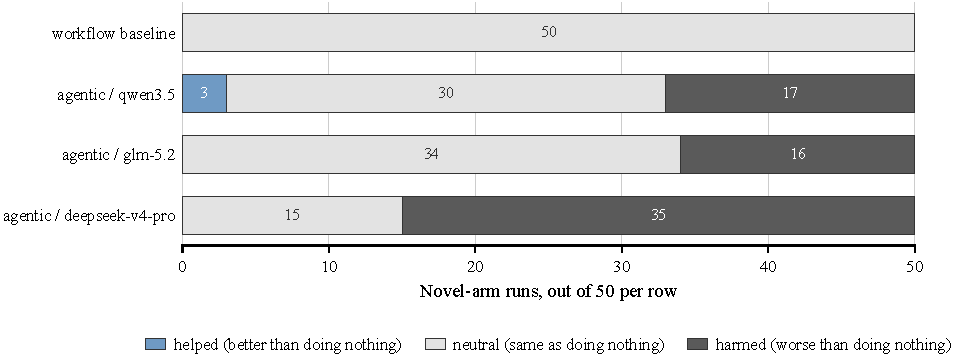
\includegraphics[width=\textwidth]{pics/critique-regret.pdf}
\caption[Null-policy regret per run]{Each novel-arm run against the null
policy, which ignores the disruption. The baseline ties it in every run. The
agentic models tie it or do worse, and three runs of 150 do better.
Exploratory. Drawn from \texttt{data/null\_policy\_regret.csv}.}
\label{fig:crit:regret}
\end{figure}

Table~\ref{tab:crit:regret} and Figure~\ref{fig:crit:regret} need to be read
together, because the two systems say different things.

\textbf{The baseline's regret is exactly zero in all 50 runs.} It gained
nothing by responding. Its response to each disruption changed no order and no
kilometre. The headline ``the workflow baseline beats the agentic system on
resident survival in every disruption tested'' is arithmetically true. It
describes a contest in which one party did not have to compete.

\textbf{The agentic regret is negative everywhere.} No cell is positive on
average; the mean is negative in all 15 model and disruption cells. Of 150
runs, three improved on the null policy, 79 tied it, and \textbf{68 came out
worse than doing nothing}. This is a harsher statement than the first
protocol's. That protocol said the agentic system lost to a better system.
Regret says it lost to inaction. A negative regret is a self-inflicted loss,
and it cannot be blamed on the scenario being hard.

The capability ordering of Section~\ref{sec:res:models} survives intact:
deepseek-v4-pro at $-0.273$, glm-5.2 at $-0.160$, qwen3.5 at $-0.100$. Under
regret it reads as how much damage the response did, not as how far behind the
baseline each model fell.

% =====================================================================
\section{The Mechanism, Corrected by Measurement}
\label{sec:crit:mechanism}

The first write-up explained the agentic deficit in prose. It said the agents
lost residents ``at the handshakes'': a driver's completion call that times out
and is never retried, a facility query that is never answered. That diagnosis
was plausible, and it was never measured. Protocol~v2 measured it, and the
measurement did not support it.

\subsection{What the Instruments Showed}

Chapter~\ref{ch:results} already reports the numbers, so they are only
collected here. Handshake closure is 0.938 over 1\,932 addressed requests, and
the three highest-volume handshakes close at 0.947, 0.970 and 0.997
(Section~\ref{sec:res:loss:handshakes}). The dominant loss mechanism is
residents who were never dispatched, with $r = -0.745$ against survival. The
loss is quantised at whole bus-loads (Figure~\ref{fig:res:delivery}). And the
full-delivery rate falls from 90\% at the minimum number of plan revisions to
32\% at six or more (Table~\ref{tab:res:commitment}).

The message layer did its job. The failure is in what the agents decided to
move, not in whether their messages arrived.

\subsection{The Alternatives That Were Ruled Out}

A diagnosis is only as strong as the alternatives it eliminates.
Table~\ref{tab:crit:ruledout} lists every candidate cause that was tested
against the 150 agentic novel runs, and the verdict on each.

\begin{table}[htbp]
\centering
\caption[Candidate causes of the agentic loss, and the verdict on each]{Candidate
causes of the agentic loss, tested against the 150 agentic novel runs.
Exploratory.}
\label{tab:crit:ruledout}
\small
\begin{tabularx}{\textwidth}{>{\raggedright\arraybackslash}p{5.2cm}>{\raggedright\arraybackslash}X}
\toprule
Candidate cause & Verdict \\
\midrule
The agents were told the wrong population & \textbf{No.} 100 residents were correctly reported in 150 of 150 runs. \\
The database message layer failed & \textbf{No.} Handshake closure is 0.938. \\
Too few missions dispatched, or the reserve bus held back & \textbf{No.} About 2.3 dispatch orders in failing and successful runs alike. Bus-2 was used in every run. \\
The scorer's arrival de-duplication removed real deliveries & \textbf{No.} De-duplicated arrival sums track sheltered residents. \\
Drivers over-claimed their headcount & \textbf{No.} 54 discrepancy rows, with $r = +0.061$ against $S$. \\
The run simply ran out of clock & \textbf{Mostly no.} Only 5 of the 19 total-loss runs recorded a dropoff after 12:00. \\
\bottomrule
\end{tabularx}
\end{table}

What is left is a \textbf{commitment failure, not a comprehension failure}. The
agents understood the disruption, addressed the right parties and had their
messages answered. What they could not do was carry one committed plan through
to delivery. Legs were re-planned while in flight, and the coordinator often
could not establish whether a leg had finished. The coordinator's own abort
messages name this directly, for example ``bus-2 reassigned to immediate
emergency dispatch, original mission never delivered'' and ``zero deliveries
across 8 transport plan revisions''.

This cuts against the architecture's own claim. Re-planning on disruption is
the capability the agentic design advertises. On these scenarios the correct
number of re-plans was zero.

\subsection{What Is Not Established}

The causal direction is open, and this thesis does not claim it. A run that is
going badly re-plans \emph{because} it is going badly. Nothing in an
observational arm separates that from re-planning causing the loss.

The abort messages show how much this matters. Each abort was classified by its
stated reason. Of 108 aborts, 57 (52.8\%) are explicit stand-downs after a
failure, 14 (13.0\%) are clearly started by a re-plan, and 37 (34.3\%) are
other. The order of classification is important. A stand-down message often
names the re-dispatch attempts that came before it, for example ``Hochbahn
unresponsive to 3 redispatch requests over 18 min''. That message is a
\emph{consequence} of the failure, not a re-plan that caused it. So the
failure response is tested first. Testing for churn first would misclassify
these messages and inflate a causal reading the design cannot support.

The experiment that would settle the direction is a
\textbf{commitment-constrained variant}: cap the number of re-plans, or forbid
cancelling a leg that is already in flight, and run it on the same scenarios
with the same models. It is one campaign and needs no new scenarios. It is
future work, not a defect of this study, and it is the most valuable follow-up
this analysis produces.

\subsection{A Lesson From Measuring Handshakes}

Measuring closure was harder than it looks, and three reading rules carry the
instrument. Each one silently zeroes a whole handshake type if it is dropped.
Agent ids are written two ways, so a driver addressed as
\code{agent-bus-driver-1} signs as \code{bus-driver-1}; exact string matching
reports closure as 0.50 instead of 0.94. The message \code{confirm_dropoff} has
two jobs: to a shelter it asks for intake, to Hochbahn it only reports progress
and expects no answer. And no clock in the log orders two agents' rows, because
each recipient stamps its own simulated time. Closure is therefore defined as a
matching between requests and replies, which is stable under any ordering, and
\textbf{no reply latency is reported at all}. The data cannot support a latency
claim.

% =====================================================================
\section{The Pre-Registered Primary Was Underpowered by Construction}
\label{sec:crit:power}

Two separate things are reported here, and they should not be merged.

\paragraph{A timing deviation.} The pre-registration named a Clopper-Pearson
interval, a scenario-level sign test and a Holm-Bonferroni correction as the
primary test for H2. None of the three existed in the code when the H2 verdict
was first written. They were implemented afterwards, once the result was known
(Amendment~15). Under the pre-registration's own rules that analysis is
exploratory. It agrees with the verdict it was checking
(Section~\ref{sec:res:novel:prereg}), which does not excuse the timing.

\paragraph{A design finding.} This is the more interesting one. At $k = 10$ the
registered aggregation could not reach conventional significance however the
data fell. A two-sided exact sign test on five scenarios cannot return a $p$
below 0.0625, even when every scenario points the same way. Ties push the floor
higher. qwen3.5 and glm-5.2 each tie two scenarios, which leaves three untied
observations and a floor of 0.250. Table~\ref{tab:res:signtest} shows that
both models sit exactly at the smallest $p$ their data could have produced.
The design would not have detected a moderate effect even if one had existed.

This is a finding about pre-registered analysis plans, not an apology for this
one. A registered primary that cannot reach significance is not a test.
Protocol~v2 draws three consequences from it:

\begin{enumerate}
\item The registered primary must be one the design can detect. The paired
  risk difference, which is continuous and far more efficient, becomes
  primary. The sign test becomes a supporting robustness check.
\item The minimum detectable effect is declared before any run. If it exceeds
  the registered margin, either $k$ rises or the claim is dropped, before data
  collection and not after.
\item Cells that fail Gate~0 are excluded from confirmatory arms by rule, not by
  judgement and not after the result is known.
\end{enumerate}

% =====================================================================
\section{The Cut-Point Sensitivity Analysis}
\label{sec:crit:sensitivity}

The protocol made a sensitivity analysis on the level cut points a
precondition on the headline. The first write-up did not contain it. The
summary said it must be reported, but printed no table, and the reporting
script never read the field. The check existed on paper and not in code.

It is now emitted, and it supports the headline (Section~\ref{sec:res:sensitivity}).
With the cut moved to 0.40, 0.50 and 0.60, every cell in the three full novel
arms keeps its median level except one, deepseek on
\code{unverified_persons_report}, which moves from 2.0 to 1.5 at 0.60. No
ordering between the agentic system and the baseline moves anywhere in the
range. The lesson is procedural: a precondition that a report asserts but does
not compute is not a precondition. It should fail the build.

% =====================================================================
\section{Limitations Declared, With the Position Taken on Each}
\label{sec:crit:limitations}

Table~\ref{tab:crit:limits} lists the six limitations that came out of
executing the design. Each is a position, not an open question, and none
requires further work before submission. The limitations declared before the
evaluation are in Table~\ref{tab:eval:scope}.

\begin{table}[htbp]
\centering
\caption{Declared limitations and the position taken on each.}
\label{tab:crit:limits}
\small
\begin{tabularx}{\textwidth}{>{\raggedright\arraybackslash}p{4.4cm}>{\raggedright\arraybackslash}X}
\toprule
Limitation & Position \\
\midrule
The novel arm was not a valid adaptability test &
Declared, and claimed as the methods contribution. The protocol's own negative
control shows the null policy at the ceiling on every scored scenario, so H2
could not have resolved in either direction (Section~\ref{sec:crit:gate0}). \\
\addlinespace
The causal direction of plan churn is open &
Future work, not a defect. Plan revisions track survival, but most aborts are
stand-downs after a failure. The commitment-constrained variant is the
experiment that would settle it (Section~\ref{sec:crit:mechanism}). \\
\addlinespace
Parity deviation 7 was still open when the campaign ran &
Closed by written re-argument, which the protocol's gate allows. The
deviation runs against the baseline, so it cannot explain a baseline win. It
could only have understated the margin (Section~\ref{sec:val:dev7}). \\
\addlinespace
42 of 87 doctrine elements have no page citation &
A limitation on the claim that the baseline is doctrine-grounded, and on
nothing else. It affects no number. 45 of 87 elements are cited to a page, the
rest are asserted by the author. \\
\addlinespace
Only one time scale ran (8.4) &
H4 was not tested. No crossover, trend or scale-dependence claim is made
anywhere. The evaluation is finished, so this is permanent. \\
\addlinespace
The registered H2 primary was implemented late &
Disclosed and labelled exploratory. Reported as a methods finding: the
registered primary was underpowered by construction
(Section~\ref{sec:crit:power}). \\
\bottomrule
\end{tabularx}
\end{table}

A second group of caveats applies to individual tables rather than to the
design. Each is disclosed where its effect is visible, and they are collected
here so that none is missed.

\begin{itemize}
\item \textbf{Levels are comparable only across the three full arms.} Partial
  model series have no clean-run reference and are capped at level 3. They are
  compared on $S$ only (Section~\ref{sec:res:models:levelcap}).
\item \textbf{Six runs shelter more residents than the ceiling admits.} The cap
  is applied at the reporting layer, not in the scorer
  (Section~\ref{sec:res:integrity:ceiling}).
\item \textbf{The novel arm's third model changed four times} after data were
  seen, so that arm's model set is exploratory
  (Section~\ref{sec:res:models:churn}).
\item \textbf{Two runs executed on a dirty working tree}, with routing changes
  that were committed later. The exclusion rules do not admit this as a reason,
  so they are kept and disclosed.
\item \textbf{28 of 168 agentic novel runs did not quiesce.} The outcome was
  decided in all of them, but a final message may be missing from the log.
\item \textbf{The cloud model tags are not version-frozen}, so no digest pins
  these results.
\item \textbf{Three asymmetries favour the baseline}: the reserve-bus
  serialisation on the agentic side, a fallback playbook that mis-frames two
  message types for the agents, and the anchor of a replacement bus leg.
  Chapter~\ref{ch:validity} states each with its direction
  (Sections~\ref{sec:val:extra} and~\ref{sec:val:reserve}). Each runs in the
  baseline's favour, so none of them can explain the agentic deficit away.
\end{itemize}

% =====================================================================
\section{What This Protocol Still Does Not Measure}
\label{sec:crit:scope}

Protocol~v2 removes nothing from the scope table of the first protocol
(Table~\ref{tab:eval:scope}). Table~\ref{tab:crit:scope} adds the limits that
v2 introduces or inherits.

\begin{table}[htbp]
\centering
\caption{What Protocol~v2 still does not measure.}
\label{tab:crit:scope}
\small
\begin{tabularx}{\textwidth}{>{\raggedright\arraybackslash}p{5.2cm}>{\raggedright\arraybackslash}X}
\toprule
Not measured & Why \\
\midrule
Whether the agentic architecture wins on a scenario that passes Gate~0 &
No such scenario has been run. Protocol~v2 makes the question askable. It does
not answer it, and nothing here licenses a claim about what would happen. \\
\addlinespace
Reply latency & No clock in the log orders two agents' rows. Closure is
measured, lag is not. \\
\addlinespace
Whether a reply was correct & Closure asks whether an answer came back, never
whether it was right. A shelter that confirms an intake it cannot hold still
counts as closed. \\
\addlinespace
Whether over-budget runs would do better at a slower clock & Only one time
scale was run. H4 was not tested and now cannot be. \\
\addlinespace
Any confirmatory claim & Every v2 instrument was written after the data were
seen. \\
\addlinespace
The baseline's coordination cost under a binding disruption & Its 13 messages
per run were measured on scenarios that asked for no re-planning. A scenario
that did would raise that number by an unknown amount. \\
\bottomrule
\end{tabularx}
\end{table}

Taken together, the chapter leaves six points for the reader.

\begin{enumerate}
\item The comparison was run on scenarios where the baseline could not lose.
  Its perfect survival is invariance, not recovery, and the no-replan control
  shows this on every scored file.
\item The agentic deficit is nonetheless real, and it is now measured more
  sharply. Against the null policy its regret is negative in every cell, and
  68 of 150 runs came out worse than doing nothing.
\item The mechanism is not the one first named. The message layer closes 94\%
  of addressed requests. The loss is dominated by residents never dispatched.
\item It is a commitment failure, not a comprehension failure. The loss comes
  in whole bus-loads, and full delivery falls from 90\% to 32\% as plan
  revisions rise. The causal direction is not established.
\item The architecture's cost is an order of magnitude higher and is now
  printed (Section~\ref{sec:res:responsetime}).
\item Whether that cost ever buys anything is untested, because no scenario in
  this thesis ever required it to. A campaign on scenarios that pass Gate~0 is
  the experiment that would find out.
\end{enumerate}

\chapter{Discussion}
\label{ch:discussion}

% ===========================================================================
% WARNING, READ BEFORE WRITING. The original skeleton of this chapter asserted
% "LLM-agent coordination degrades more gracefully than pre-scripted
% workflows". THAT IS THE OPPOSITE OF WHAT HAPPENED. It was the proposal's
% expected finding, written in before the data existed. It has been removed.
% If any draft still carries it, delete it.
% ===========================================================================

\section{Interpretation}
\label{sec:disc:interpretation}
% Answer RQ1 and RQ2 directly, in operational terms, then stop.
%
% RQ1: No. The baseline saved every resident in every novel run; the best
% agentic configuration saved 90 %. Gate 1 fails 26 of 27 cells.
% Sharpen it with the regret result: the agentic system did not merely lose to
% a better system, it lost to INACTION. 68 of 150 runs came out worse than
% doing nothing.
%
% BUT SAY WHAT THE BASELINE'S WIN IS AND IS NOT. Its S = 1.000 is invariance,
% not recovery. It gained nothing by responding: regret exactly zero in all 50
% runs. Never write that it "adapted" or "replanned better"
% (Chapter~\ref{ch:critique}).
%
% RQ2: The deficit is a COMMITMENT failure, not a comprehension failure.
% Walk the eliminated alternatives, because the elimination is what makes the
% claim credible: wrong population (no, 150/150 correct), message layer (no,
% 93.8 % closure), too few missions or a withheld reserve (no, ~2.3 dispatches
% either way, bus-2 used in 100 % of runs), scorer dedup (no), driver
% over-claiming (no), running out of clock (mostly no).
% Then the positive evidence: the loss is QUANTISED at whole bus-loads, and
% plan revisions band monotonically against delivery.
%
% The rubric is where "they can reason, they cannot finish" is visible:
% parity on the five criteria about DECIDING, short on five about CLOSING THE
% LOOP. Do not round that to "decision-quality parity" - it is a split.

\section{The Capability Ordering}
\label{sec:disc:capability}
% Mean RD narrows with model capability: deepseek -0.27, glm-5.2 -0.16,
% qwen3.5 -0.10, consistent across all five novel disruptions.
% Under the regret reading this is "how much damage the response did", not
% "how far behind the baseline it fell". Say it that way.
% DO NOT EXTRAPOLATE past qwen3.5. The design does not support it, and there is
% no capability threshold observable within the final model set.
% qwen3.5 also strands far fewer residents than the others (2.0-5.0 per 100 vs
% 10-22.5), so its deficit has a materially different shape from deepseek's.

\section{Trade-offs}
\label{sec:disc:tradeoffs}
% The baseline wins response time, cost and determinism, and it also won the
% primary outcome. Report that without softening.
% The agentic cost is an order of magnitude: 9-10x messages per resident
% delivered, ~800k tokens, 1.8-2.7x wall-clock.
% The honest framing: this is a cost with no demonstrated benefit ON THESE
% SCENARIOS. Whether it ever buys anything is untested here, because no
% scenario in this thesis required it to.

\section{Transferability}
\label{sec:disc:transfer}
% Which domains share the two conditions this case was built around: a
% disruption space too large to pre-enumerate, and heterogeneous actors holding
% local information.
% CAUTION. This thesis did not demonstrate an agentic advantage under those
% conditions. What transfers is the METHOD and the DIAGNOSIS, not a positive
% result. Generalise the design considerations
% (Chapter~\ref{ch:design}), not the architecture's performance.

\section{Threats to Validity}
\label{sec:disc:validity}
% Construct, internal, external, conclusion validity.
% Construct validity of the primary DV is argued in
% Section~\ref{sec:eval:construct}; parity and the deviations are
% Chapter~\ref{ch:validity}; treatment validity is
% Chapter~\ref{ch:critique}. Summarise, do not repeat.

\section{Limitations}
\label{sec:disc:limits}
% State these plainly. Being caught not having noticed is worse than declaring.
% The full list with the position on each is in Chapter~\ref{ch:critique};
% keep this section short and point there.
%   - single case: one facility, one city, one hazard
%   - one SIM_TIME_SCALE (8.4), so H4 was not tested
%   - k = 10 (NOT the ~30 the proposal planned; Amendment 1 set it on budget
%     and precision grounds after power.py showed no k buys H1)
%   - the scenario-scaling sweep was never run
%   - no equity dimension: the resident population is homogeneous by
%     declaration, so a max-min subgroup difference is identically zero
%   - residents modelled as a passive count, not as agents
%   - the feasibility ceiling complicates cross-study comparison
%   - LLM nondeterminism; :cloud tags are not version-frozen
%   - the novel arm's third model changed four times, so that arm is
%     exploratory under PREREGISTRATION sec.0

\section{Lessons Learned}
\label{sec:disc:lessons}
% Short. What would be built differently, as a bridge into
% Chapter~\ref{ch:design}, which carries the generalisable version.
% Resist duplicating that chapter here.


% RQ4: the generalisable deliverable. Follows the discussion because it
% generalises from it, and precedes the conclusion because the conclusion
% points back at it.
\chapter{Design Considerations for Agentic Emergency Simulation}
\label{ch:design}

% ===========================================================================
% THIS CHAPTER ANSWERS RQ4 and carries the generalisable contribution. It is
% where the thesis stops being about one nursing home in Hamburg.
%
% SOURCES: EVALUATION_PROTOCOL_V2 sec.11.4 and sec.16, RESULTS sec.4-5,
% PARITY.md, and the ADRs (which are the design record of what was decided and
% what it cost).
%
% VOICE. Each consideration is a claim EARNED BY THE EVIDENCE in this thesis,
% not advice in general. For every one: state the consideration, give the
% measurement from this study that motivates it, then state its limit. If a
% consideration has no number behind it, mark it as a judgement, not a finding.
% ===========================================================================

\section{Commit Before You Re-Plan}
\label{sec:design:commitment}
% THE CENTRAL LESSON, and the one with the most evidence behind it.
% An architecture whose advertised capability is "re-plan when disrupted" must
% also answer: what stops it re-planning? On these scenarios the correct number
% of re-plans was zero, and runs that re-planned the minimum delivered everyone
% 90 % of the time against 32 % at six or more revisions.
% Design implication: a plan leg already in flight needs a commitment boundary.
% Re-planning must be an explicit, costed act, not the default response to any
% new message.
% STATE THE LIMIT HONESTLY: the causal direction is not established. 53 % of
% aborts are post-failure stand-downs, so a failing run plausibly re-plans
% BECAUSE it is failing. This is a design consideration supported by a strong
% correlation, not a demonstrated cause. See Chapter~\ref{ch:critique}.

\section{Closing the Loop Is Not the Same as Finishing the Job}
\label{sec:design:closure}
% The message layer worked: 93.8 % handshake closure over 1,932 addressed
% requests. The residents were still not delivered.
% Design implication: message-level health metrics are necessary and nowhere
% near sufficient. Instrument DELIVERY, not correspondence. A coordinator that
% cannot establish whether a leg finished will re-plan a leg that succeeded.
% Evidence: the coordinator's own abort texts name exactly this
% ("plan revision 2 claimed both runs drop off by 10:50, but no
% transport_complete arrived").

\section{Make the Resource Allocation Genuinely Bind}
\label{sec:design:binding}
% From the case design (Chapter~\ref{ch:casestudy}): 100 residents, 2 buses at
% 50 seats, 2 shelters at 60 beds. One bus and one shelter could have absorbed
% the whole mission, and then there would have been nothing to allocate.
% Design implication: if the scenario's resources are slack, the simulation
% measures nothing about coordination. Size the fit deliberately and say so.

\section{Decide What a Reserve Means, and Enforce It on Both Sides}
\label{sec:design:reserve}
% The reserve bus is the clearest example in this thesis of a semantic
% declared in a scenario file and honoured by only one of the two systems.
% The agentic Hochbahn honours role: reserve and serialises; the baseline's
% run_schedule never reads role and flies bus-2 in parallel from t0.
% Design implication: any semantic a scenario declares must be either enforced
% by the shared substrate or declared as a deviation with its direction.
% Cross-reference Section~\ref{sec:val:reserve}; do not re-argue it here.

\section{Build the Negative Control Before the Treatment}
\label{sec:design:gate0}
% The single most transferable methodological point, and it belongs here as
% well as in Chapter~\ref{ch:critique}.
% A disruption scenario is only a disruption if a system that IGNORES it scores
% worse than one that responds. Test that first, with a no-replan control,
% before spending a campaign on it.
% Evidence: on all five novel scenarios the no-replan control committed
% byte-identical orders and scored the identical level.

\section{Cost Is Architectural, Not Incidental}
\label{sec:design:cost}
% The agentic side spends 9-10x the messages per resident delivered, ~800k
% tokens, and 1.8-2.7x the wall-clock budget. Agentic wall latency per run
% ranges 763 s to 3,810 s; the baseline's LLM latency is 0.0 s by construction.
% Design implication: budget this from the start and decide what it must buy.
% THE OPEN QUESTION TO NAME: whether that cost ever buys anything is untested
% here, because no scenario in this thesis ever required it to.

\section{Determinism, Variance, and What an Evaluation Can See}
\label{sec:design:variance}
% The baseline is a deterministic reference spike; the agentic side is not.
% Report variance as an honest cost of the approach.
% Practical notes earned the hard way in this project:
%   - :cloud model tags are not version-frozen; no digest pins these results.
%   - Retrying malformed LLM output would give a weak model a second attempt a
%     strong one never needed. This system deliberately does not retry.
%   - k = 10 could not detect a moderate effect. Size the design, or report
%     that you did not.

\section{What These Considerations Do Not Cover}
\label{sec:design:scope}
% Close on scope, briefly and without padding. Single case, single city, one
% time scale, homogeneous resident population (so equity is undefined by
% declaration), residents modelled as a passive count.
% These considerations are grounded in one evaluation of one architecture on
% one case. Say that, and resist generalising past it.

\chapter{Conclusion and Future Work}
\label{ch:conclusion}

% ===========================================================================
% WARNING. The original skeleton claimed contribution 1 as "EMPIRICAL:
% LLM-agent coordination degrades more gracefully than a doctrine-grounded
% workflow baseline under novel disruption." THAT IS THE OPPOSITE OF THE
% RESULT. It was the proposal's expectation. It has been replaced below.
% ===========================================================================

\section{Summary}
\label{sec:concl:summary}
% Restate the four research questions and answer each in two or three
% sentences. No new evidence here, and no hedging.
%   RQ1 Can it beat the scripted baseline? No, and it also loses to a null
%       policy. Chapters~\ref{ch:results} and \ref{ch:critique}.
%   RQ2 Why not? A commitment failure, not a comprehension failure.
%       Chapter~\ref{ch:discussion}.
%   RQ3 What would have to change? Constrain commitment; test on scenarios
%       that discriminate. Section~\ref{sec:concl:future}.
%   RQ4 What should a designer consider? Chapter~\ref{ch:design}.
% Then the four engineering sub-questions, one line each, pointing at
% Chapters~\ref{ch:data}, \ref{ch:agentic}, \ref{ch:eval} and \ref{ch:results}.

\section{Contributions Revisited}
\label{sec:concl:contributions}
% The four contributions from Section~\ref{sec:intro:contributions}, restated
% against the evidence that was actually produced:
%
%  1. ARTEFACT. Built and running: 10 agents across 8 organisations, Postgres
%     as single source of truth and active broker, plus a doctrine-grounded
%     baseline at audited parity (Chapter~\ref{ch:validity}).
%
%  2. EMPIRICAL, AND NEGATIVE. 310 scored runs over 7 scenarios. The agentic
%     architecture does not outperform the scripted baseline on resident
%     survival, and underperforms a null policy. This is a result, and it is
%     reported as one.
%
%  3. DIAGNOSTIC. The deficit is located and measured: commitment, not
%     comprehension. This is the part a future builder can act on.
%
%  4. METHODOLOGICAL. The shared append-only event log as the backbone of a
%     fair, auditable, replayable comparison; and Gate 0, the treatment-
%     validity check that catches a non-discriminating disruption before it is
%     scored. A protocol that found its own primary arm degenerate and
%     specified the gate that would have caught it.

\section{Future Work}
\label{sec:concl:future}
% RQ3 lives here. Lead with the one experiment that matters and rank the rest.
%
% 1. THE COMMITMENT-CONSTRAINED VARIANT. The highest-value follow-up this
%    analysis produces. Cap re-plans, or forbid cancelling a leg already in
%    flight; run against the same scenarios under the same models. One
%    campaign, no new scenario authoring. It is also the experiment that would
%    settle the causal direction this thesis explicitly leaves open.
%
% 2. SCENARIOS THAT PASS GATE 0. Author disruptions where a no-replan control
%    demonstrably fails, so adaptation has something to prove. Until that runs,
%    "can an agentic architecture ever beat a scripted one" is open, not
%    answered.
%
% 3. A DESIGN THE EVALUATION COULD SEE. A larger k (10 could not detect a
%    moderate effect), more than one SIM_TIME_SCALE (H4 was never tested), and
%    a model set fixed before the arm runs.
%
% 4. Longer-horizon: resident-level agents, an equity dimension in the rubric,
%    compound and cascading disruptions, multi-case replication beyond a single
%    facility, other cities and hazards.


% --- Bibliography --------------------------------------------------
\newpage
\printbibliography[heading=bibintoc]

% --- Back matter ---------------------------------------------------
\appendix
\chapter{Frozen Evaluation Artifact}
\label{app:frozen}
% THE AUDIT TRAIL. Everything frozen before evaluation day, with git commit
% hashes and dates:
%   - the Recovery-Outcome Rubric levels and thresholds
%   - the scoring script version
%   - the workflow baseline tag (Section~\ref{sec:wf:freeze})
%   - the parity conformance test result
% This appendix is what makes the preregistration claim checkable rather than
% merely stated.

\chapter{Disruption Brief}
\label{app:brief}
% The characteristics-only brief given to the external supplier, reproduced in
% full. Shows what was and was not communicated, which is the firewall evidence.

\chapter{Adjudication Log}
\label{app:adjudication}
% Written record of every residual edge call the deterministic scorer could not
% settle (mainly level-0 vs level-1), with the reasoning for each.

\chapter{Database Schema (DDL)}
\label{app:ddl}
% TODO: \lstinputlisting[language=SQL]{...}

\chapter{Agent Prompts}
\label{app:prompts}
% TODO: CORE system prompt + the three event playbooks, per agent.

\chapter{Scenario Definitions}
\label{app:scenarios}
% TODO: \lstinputlisting of the scenario JSON files.

\chapter{Reproducibility}
\label{app:repro}
% How to run the systems and the harness. Model digests, environment variables
% (SIM_TIME_SCALE, OLLAMA_MODEL, ORS_API_KEY), migrations, seeds.


\chapter*{Declaration of Authorship}
\addcontentsline{toc}{chapter}{Declaration of Authorship}

I hereby declare that I have written this thesis independently and without
the use of any sources or aids other than those explicitly cited. All passages
taken verbatim or in substance from published or unpublished works are
acknowledged as such. This thesis has not been submitted, in the same or a
similar form, to any other examination authority.

\vspace{2cm}

\noindent
Ilmenau, \today \hfill \saauthor


\end{document}
